

\documentclass[11pt]{article}
% \documentclass[10.8pt, a4paper, USenglish, twocolumn]{article}

\usepackage{isaks_template} % Contains all included packages. See isaks_template.sty.

% latex margins
% \linespread{1.5}
% \newgeometry{vmargin={15mm}, hmargin={25mm,37mm}}
\newgeometry{vmargin={15mm}, hmargin={30mm,30mm}}
%
% \title{Project Thesis\\ Solving the Biharmonic Equation using \\ a Continuous Interior Penalty Method}
% \author{Isak Hammer, \\[1cm]{\small Advisor: André Massing} }

\begin{document}


\begin{titlepage}
    \begin{center}
        \vspace*{1cm}

        \Huge
        \textbf{Master Thesis}

        \vspace{0.5cm}
        \Large
        Solving Cahn-Hilliard equation using a CutCIP method   \\

        \vspace{1.5cm}

        \textbf{Isak Hammer} \\
        \vspace{0.5cm}
        Supervisor: André Massing \\
        \vspace{0.5cm}
        \today


        \vfill

        \vspace{0.8cm}

        % \includegraphics[width=0.5\textwidth]{figures/front_page/molly.jpeg}\\

        \Large
        Department of Mathematical Sciences\\
        Norwegian University of Science and Technology\\

    \end{center}

\end{titlepage}
    % \begin{titlepage}
    %     \maketitle
    %     \begin{figure}
    %     \centering
    %     % 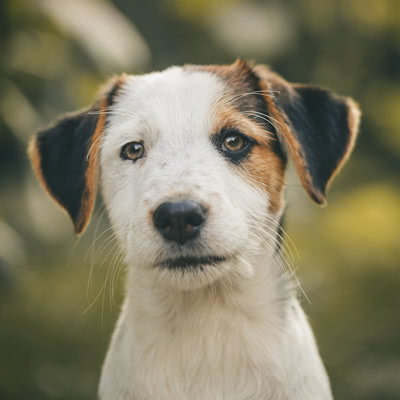
\includegraphics[width=0.5\textwidth]{figures/front_page/dog.jpg}\\
    %     \includegraphics[width=0.5\textwidth]{figures/front_page/molly.jpeg}\\
    %     \end{figure}
    %     \thispagestyle{empty}
    % \end{titlepage}


    \newpage


    \section{Introduction}\label{sec:introduction}

Cell membranes are the foundation of the origin of life, but also linked to the dynamics of virus al infections and genetic mutations since it controls what substances that can exit or enter the cell \cite{ hurley2010membrane}. In fact, a good
understanding of the cell membrane is important of engineering proteins to manipulate various intracellular processes in living systems \cite{rojas1998genetic}.

One of the primary components of the cell membranes are lipids which serve many different functions. A key function is that it is consisting of a bilayer of lipids which controls the structural rigidity and the fluidity of the membrane. Thus, elastic
bending forces, temperature and diffusion is essential on how a cell membrane will evolve \cite{udo97,neidleman87}.


\subsection{Elastic bending energy on evolving surfaces}%
\label{sub:willmore_flow}

Assuming that the system is a single-phase system, i.e., the lipids are uniformly distributed, can the elastic bending energy be modelled using the Canham-Helrich energy functional \cite{helfrich1973elastic, wang08, udo97}. Let us denote $b_{b},
b_{k}$ and $H_{0}$ as parameters based on physical models, then can the energy functional be denoted as,
\begin{equation}
\label{eq:CH}
\mathcal{E} _{CH}\left( \Gamma\left( t \right)   \right) =   \int_{\Gamma  }^{}  b_{b} \left( H- H_{0} \right) ^{2} + b_{k} K
.\end{equation}
Here is $H =  \kappa_1 + \kappa_2 $ denoted as the mean curvature and $K = \kappa_1 \kappa_2$ as the gaussian curvature with respectively and $\kappa_1$ and $\kappa_2$ as principal curvatures. $\Gamma \left( t
\right) = \Gamma  $ is here an evolving surface in $\mathbb{R} ^3$, for more info see section \ref{sec:background}.  Using the Gauss-Bonnet theorem can it be shown that the problem above is equivalent to the so-called Willmore energy
functional \cite{montiel2009curves, willmore1996riemannian},

\begin{equation}
\label{eq:WE}
\mathcal{E} _{W} \left( \Gamma\left( t \right)   \right) = \int_{\Gamma  }^{} \frac{1}{2} H ^2
.\end{equation}

This is a well known problem in the mathematical community \cite{ topping2000towards, marques2014willmore,link2013gradient,kuwert2012willmore}. In fact, it is a mathematical tool used to study the geometry of surfaces because it can be used to study
the diffeomorphism from a initial surface to a minimal energy configuration, which are surfaces with the least possible area for a given boundary. This is important in many areas of mathematics, including differential geometry, topology and mathematical physics \cite{koerber2021area,jakob2022singularities, rupp21}.

It has been established many numerical methods for for shape optimization problems \cite{sokolowski1992introduction,ito2008variational}, evolving surface partial differential equations (PDE) \cite{dziuk2013finite, dziuk2007finite,
binz2022convergent, barrett2007parametric, barrett2007variational, kovacs2019convergent, lehrenfeld2018stabilized} and specific
algorithms for the Willmore energy problem \eqref{eq:WE} \cite{palmurella2022parametric, dziuk2008computational, bonito2010parametric,  kovacs2021convergent, hu2022evolving}.

\subsection{Two-phase separation modelling on predefined evolving surfaces }%
\label{sub:two_phase_seperation_modelling_on_surfaces_}

It also turns out that the lipids often accumulate into so-called lipid rafts which serves as a rigid platform for proteins with special properties such as intracellular trafficking of lipids and lipid-anchored proteins \cite{ miller2020divide}. Modelling of
lipid rafts formation can be modelled as a two-phase separation problem based on minimization of the Ginzburg-Landau energy functional \cite{yushutin19},
\begin{equation}
\label{eq:GL}
\mathcal{E}_{GL}  \left( c   \right) = \int_{\Gamma\left(t  \right)   }^{}\Psi \left( c \right) + \frac{\gamma}{2} \left\lvert \nabla c \right\rvert^{2} ,
\end{equation}
which describes the chemical energy for a concentration $c: \Gamma\left( t \right)  \times \left[ 0,T \right] \mapsto  \left[ 0,1 \right]  $. Here is $ \Psi \left( c \right): \mathbb{R} \mapsto \mathbb{R} $ denoted as a nonlinear scalar chemical potential function. Keep in mind that unlike
the Willmore energy functional \eqref{eq:WE}, where the $\Gamma\left( t \right)  $ is determined by the elastic properties, should the energy functional \eqref{eq:GL} be interpreted as a chemical diffusion problem a predefined evolving domain $\Gamma \left( t \right) $.
Usually is this problem solved by deriving equivalent variants of partial differential equations (PDE) such as Allen-Cahn equation (or Cahn-Hilliard equation if the total concentration is globally conserved) on evolving domains. For further details,
see \cite{yushutin19,
udo97, ratz16,Gera2017, caetano21, elliott2015evolving}.

\subsection{Multiphysics problems on evolving surfaces}%

Ultimately will the cell membrane consists of interaction several kinds of physics (temperature, elasticity, chemical diffusion, internal fluid pressure etc.) \cite{udo97}. Hence, being able to model several processes may give unforeseen results.

An interesting example is to couple the energy functionals \eqref{eq:GL}  and \eqref{eq:CH}, since the lipid-rafts formation is said to change the elasticity properties of the membrane, may be a good model for how cell membranes evolve to specific shapes or execute cell division. One way
to couple the energy functionals is to let the parameters $b_{b}, b_{k}$ and $ H_{0} $ be some function of the time dependent concentration $c$, i.e.,
\[
    \begin{split}
        \mathcal{E}_{CHGL} \left( \Gamma\left( t \right) ,c\left( t \right)    \right) =  & \int_{\Gamma  }^{}  b_{b}\left( c \right)  \left( H- H_{0}\left( c \right)  \right) ^{2}  \\
        & + \int_{\Gamma   }^{} b_{k}\left( c \right)  K \\
        &+ \int_{\Gamma   }^{}\Psi \left( c \right) + \frac{\gamma}{2} \left\lvert \nabla c \right\rvert^{2} ,
    \end{split}
\]
For more information, see \cite{elliott2010surface}.

Recently have some authors also coupled diffusion processes and the so-called mean curvature energy, see \cite{burger2021interaction, elliott2022numerical}. It is well known that lipids travels
along the cell membrane in a fluidic manner, hence, it is also of interest to couple the Ginzburg-Landau energy functional \eqref{eq:GL} (or more specifically the Cahn-Hilliard equation) with the Navier-Stokes equation. Some methods has been proposed
methods for solving the problem on surfaces
and evolving surfaces, but it remains a field of active research \cite{olshanskii2022comparison}. As far as a author knows, coupling the Canham-Helrich energy functional \eqref{eq:CH}, Ginzburg-Landau energy functional \eqref{eq:GL}  and Navier-Stokes equation remains a open problem.

Some physical processes may require constant area and volume. This can simply be added by introducing respectively area and volume functionals, see \cite[Definition 2.5]{muller2013volume}.

Until now have all the models assumed that the membrane has no difference in internal and external pressure. As a matter of fact, osmotic pressure can be introduced by adding a energy functional using the van't Hoff formula. Let $V_{p}$ be the volume
of a closed evolving surface $\Gamma \left( t \right) $, we can then model the difference of internal and external pressure as,
\[
\Delta P \left( V_{p} \right) = P_{in} - P_{out} = iRT\left( \frac{n}{V_{p}} - \overline{c}  \right),
\]
where $i, R, T, \overline{c} $ and $n$ are the van't Hoff index, ideal gass constant, temperature , ambient molar concentration and molar amount of the enclosed solute. Then the energy
functional have the form,
\[
\mathcal{E} _{p}\left( \Gamma    \right)  = \int_{\Gamma   }^{   } \Delta P\left( V_{p} \right) ,
\]
For more information, see \cite{zhu2022mem3dg}.


\subsection{Outline of this report}%
\label{sub:outline_of_this_report}

The long-term goal would be to solve the multi-physics problems above. However, many of the problems above is fairly complicated to solve numerically and requires sophisticated techniques. Hence, in this report we focus on the latest research withing
the numerical methods of finding the minima of the energy functional \eqref{eq:WE}. However, we will first establish notation by including a section for definitions and important results from differential geometry and shape derivatives. We will then derive the
underlying dynamics system of evolutionary system dynamics using the gradient flow technique inspired by shape optimization methods based on the work done in \cite{ dougan2012first}. Lastly, we will establish the numerical methods of the system
dynamics by applying recent methods using an evolutionary surface finite element method (FEM) \cite{kovacs2021convergent, hu2022evolving}.





    %%% old
    % 
\newpage
\section{Unfitted cut discontinuous Galerkin method for the Poisson problem}%
\label{sec:elliptic}

\subsection{Poisson problem}%
\label{sub:possion_problem}
We will first consider the continuous Poisson problem. Let $f \in H^1( \Omega ) $ and $g \in H^{\frac{1}{2}}( \Gamma ) $ and $\Omega  \in \mathbb{R} ^{d}$ . We then define the strong formulation of the Possion problem to be \[
\begin{split}
    -\Delta u &= f \quad  \text{in }\Omega  \\
     u &= g  \quad \text{on } \Gamma    \\
\end{split} .
\]
Let us define the Hilbert spaces $V=H^{1}( \Omega ) $,   $V_{g} = \left\{ v \in H^{1}( \Omega ): v \mid _{\Gamma } = g \right\} $, the bilinear form $a: V \times V  \to \mathbb{R}  $ and the linear form $l: V'\to \mathbb{R}  $ s.t. \[
a( u,v) = ( \nabla u, \nabla v) _{\Omega }, \quad l( v) = (f,v)_{\Omega }.
\]
We say the weak formulation is to find a $u \in V_{g}$ so this equation holds  \[
a( u,v) = l( v), \quad  \forall v \in V
\]
\subsection{CutFEM }%
\label{sub:cutfem}

One of the key element to unfitted methods is that is relying on a background mesh. Let $\widetilde{\Omega }$ as a background domain with a corresponding shape regular and quasi-uniform background mesh $\widetilde{\mathcal{T}}_{h} $. We will assume we
have a physical domain $\Omega
\subset \widetilde{\Omega }$ with a corresponding $\Gamma \in C^2 $ boundary. For $\mathcal{T}_{h} $ we define a the so-called active mesh
$\mathcal{T} _{h} \subset \widetilde{\mathcal{T} }_{h}$ consisting of those elements that intersect with the interior of $\Omega^{\circ } = \Omega  \setminus \Gamma   $. That is,\[
\mathcal{T }_{h} = \left\{ T \in  \mathcal{T}_{h}  \mid  T \cap \Omega \neq \emptyset   \right\}.
\]
The set of interior facets in $\mathcal{T}_{h} $ is defined as $\mathcal{F}_{h} $.
Let the submesh $\mathcal{T}_{\Gamma } \subset \mathcal{T}_{h}  $ consisting of all cut elements, \[
\mathcal{T} _{\Gamma  } = \left\{ T \in \mathcal{T} _{h}  \mid  T \cap  \Gamma  \neq \emptyset  \right\}.
\]

\todo[inline]{ Wrap the above definitions into definitions blocks.}

We denote the discrete to function space $V_{h}$ to be the broken polynomial space of order $k$, that is, $V_{h} := \mathcal{P}^{k}( \mathcal{T}_{h} )  $.


Let the bilinear form $a_{h}: V_{h} \times V_{h} \to \mathbb{R} $  and the linear form $l_{h}: V_{h} \to \mathbb{R} $. We denote the symmetric interior penalty discontinuous Galerkin Poisson (DG Poisson)  formulation to be

\begin{equation}
\label{eq:poisson_DG}
\begin{split}
    a_{h}( v,w)  = &( \nabla v, \nabla w)_{\mathcal{T} _{h} \cap \Omega } - ( \partial _{n} v,w)_{\Gamma } - ( v, \partial _{n} w)_{\Gamma } + \beta ( h^{-1} v,w)_{\Gamma } \\
    & - ( \mean{ \partial _{n} v }  , \jump{ w }  ) _{\mathcal{F} _{h} \cap \Omega } - ( \jump{ v }  , \mean{ \partial _{n} w }  )_{\mathcal{F} _{h}} + \beta ( h^{-1} \jump{ v }  , \jump{ w }  )_{\mathcal{F}_{h}\cap \Omega  } \\
    l_{h}( v)  &=  ( f,v) _{\mathcal{T} _{h} \cap \Omega } - ( \partial _{n} v,g) _{\Gamma } + \beta ( h^{-1} g,v)_{\Gamma }
\end{split}
\end{equation}
For more information about the derivation, see \cite[Chapter 4.2]{pietro2012}. Remark that this formulation is defined on unfitted meshed and, thus, imposing Nitsche penalty to fulfill the boundary condition.
\todo[inline]{ Need source of the derivation or maybe need to to it myself }
However, to show well-posedness will we later see that it is necessary to add a stability term . Hence, the symmetric interior penalty cut discontinuous Galerkin Poisson (CutDG Poisson) formulation,
\[
A_{h}( u, v) := a_{h}( u, v) + g_{h}( u_{h}, v) = l_{h}(v)
\]
We denote the stability term $g_{h}: V_{h} \times V_{h} \to \mathbb{R} $ as the so-called ghost penalty term.

\begin{definition}[CutDG Poisson problem]
    \label{def:cutdg_poisson_problem}

We denote the CutDG Poisson problem as follows; to find a unique $u_{h} \in V_{h}$ s.t.  \[
A_{h}(u_{h}, v ) = l_{h}( v)  \quad \forall  v \in V_{h}.
\]
\end{definition}

Our main goal is to determine the necessary stability criteria for the ghost penalty term for the CutDG Poisson problem to be well-posed. We can then apply these criteria to engineer a ghost penalty to handle this problem. For convenience will we make some assumptions on our problem.


\begin{assumption}[G1]
    \label{as:G1}
    The boundary $\Gamma $ is $C^{2}$.
\end{assumption}

\begin{remark}
In most applications is $\Gamma $ represented with a level-set function, that is a sufficiently smooth function $\phi ( x)  = 0$. There exists several methods to discretize this properly s.t. it can we can compute the integral over the cut elements.
    However, to simplify the analysis will we assume the numerical contributions of the cut elements consisting of $\mathcal{T}_{h} \cap \Gamma   $ and $\mathcal{F}_{h} \cap \Omega  $ to be exact.
\end{remark}


\begin{assumption}[G1]
    $\mathcal{T}_{h} $ is mesh conform, quasi-uniform and shape regular.
\end{assumption}

\begin{assumption}[G3]
    For $T \in \mathcal{T} _{\Gamma   }$ there is a path $P$ of $diam(P) \lesssim h$ which contains $T$ and an element $T'$ with a "fat" interaction satisfying $\left\lvert T' \cap \Omega  \right\rvert \ge c_{s} \left\lvert T'  \right\rvert _{d}$
    \todo[inline]{ Don't understand this definition}
    \todo[inline]{ Define patch in mathematical background. }
\end{assumption}


\subsection{Bounded and coercive}%
\label{sub:norms}

Our goal is to show that the problem \ref{def:cutdg_poisson_problem} is well posed. We can do this by applying Lax-Milgram theorem \ref{def:lax-milgram} by showing that the bilinear form $A_{h}$ is bounded and coercive.

First of all, to be able to prove boundedness we need to define norms.
We may define the norms for $v \in V_{h}$ to be the following,
\[
\begin{split}
    \| v \|_{ a_{h} }^{ 2 }  & = \| \nabla v \|_{ \mathcal{T} _{h} \cap \Omega  }^{ 2 } + \| h^{\frac{1}{2}} \jump{ v }   \|_{ \mathcal{F} _{h} }^{ \mathcal{F} _{h} \cap \Omega   } \\
    \left\lvert v \right\rvert _{g_{h}}^{2} & = g_{h}( v,v)  \\
    \| v \|_{ A_{h} }^{ 2 } &= \| v \|_{ a_{h} }^{ 2 } + \left\lvert v \right\rvert_{g_{h}}     \\
\end{split}
\]

While for $v \in H^2( \mathcal{T} _{h}) + V_{h}$ we define the following norm,\[
\| v \|_{ a_{h},* }^{ 2 } = \| v \|_{ a_{h} }^{ 2 } +   \| h^{\frac{1}{2}} \jump{ \partial _{n} v }    \|_{  \mathcal{F} _{h} \cap \Omega }^{  2} + \| h^{\frac{1}{2}} \partial _{n} v \|_{ \Gamma  }^{ 2 }
\]






    %%%

    
\section{Mathematical Background}%
\label{sec:mathematical_background}

In this section, we revisit the established definitions and provide a brief overview of Sobolev spaces. Afterward, we briefly review the finite element method and discuss the necessary tools required for calculating a priori estimates.


\subsection{Sobolev spaces}%
\label{sub:notation}

We will in this report assume $\Omega $ to be a compact and open set in $\mathbb{R} ^{d}$. Let $p \in \mathbb{R} $, $ 1 \le  p \le  \infty$, and  define the space $L^{p}\left( \Omega  \right) $ to be the set of all measurable functions $u: \Omega  \mapsto \mathbb{R} $ such that
$\left\lvert f \right\rvert ^{p}$ is Lebesgue integrable, i.e,

\begin{equation*}
    L^{p}\left( \Omega  \right) = \left\{ u: \Omega \mapsto \mathbb{R}  \mid \int_{\Omega }^{} \left\lvert u \right\rvert ^{p} d \Omega  < \infty  \right\}
.\end{equation*}
Let $u \in L^{p}\left( \Omega  \right) $. We define the integral norm of order $p$ to be \[
\| u \|_{ L^{p}\left( \Omega  \right)  }^{  }  = \left( \int_{\Omega }^{} \left\lvert u \right\rvert ^{p} dx  \right) ^{\frac{1}{p}}.
\]

The following definition for derivatives is employed.
For $d$ dimensions of order $k$ we define the multi-index $\alpha  = ( \alpha _{1}, \ldots, \alpha _{d})  $ with the absolute value $\abs{ \alpha  } = \sum_{i=1}^{d}  \alpha _{i} = k $ s.t.
\begin{equation}
    \label{eq:der}
\partial ^{\alpha} u = \frac{\partial ^{ \alpha_{1}  }  } {\partial^{} x_{1}^{\alpha _{1}}  } \ldots \frac{\partial ^{ \alpha_{d}  }  } {\partial^{} x_{d}^{\alpha _{d}}  } u \quad  \text{for }u \in C^{\left\lvert \alpha  \right\rvert }( \Omega )
\end{equation}

  Let $k\ge 0$ be an integer and let $1 \le  p <  \infty$ be a real number, then the Sobolev space $W^{k,p}( \Omega ) $ is defined by
  \begin{equation}
W^{k,p}\left( \Omega  \right) = \left\{ u \in L^{p}\left( \Omega  \right)  \mid  \partial ^{\alpha } u \in L^{p}\left( \Omega  \right)  \forall \alpha : \left\lvert \alpha  \right\rvert  \le k \right\}.
  \end{equation}
with the corresponding norm
\begin{equation}
\| u \|_{ W^{k,p}\left( \Omega  \right)  }^{  }  = \left(   \sum_{j = 0}^{k}  \left\lvert u \right\rvert ^{p} _{  W^{j,p}\left( \Omega  \right) } \right)^{\frac{1}{p}} .
\end{equation}
Here the seminorm is defined such that $ \left\lvert u \right\rvert _{W^{k,p}( \Omega  ) }^{} =  ( \sum_{\left\lvert \alpha  \right\rvert  = k}^{} \| \partial ^{\alpha }u \|_{ L^{p}( \Omega )   }^{ p } )^{\frac{1}{p}} $.

For shorthand notation, we denote
\begin{equation}
    \begin{split}
\| \cdot \|_{k,p}^{  } & = \| \cdot  \|_{k,p,\Omega   }^{  } = \| \cdot  \|_{ W^{k,p}( \Omega )   }^{  }, \\
   \abs{ \  \cdot \ }_{k,p}^{  } &= \abs{ \   \cdot \ }_{k,p,\Omega   }^{  } = \abs{ \  \cdot \ }_{ W^{k,p}( \Omega )   }^{  },
    \end{split}
\end{equation}

Since $p=2$ is frequently used in this report, we also define for convenience a compact notation $\| u \|_{ \Omega  }^{  }  = \| u \|_{ L^{2}\left( \Omega  \right)  }^{  } $ and $H^{m}( \Omega ) = W^{m,2}( \Omega )  $ such that,
\begin{equation}
\begin{split}
\| \cdot  \|_{H^{m}( \Omega )   }^{  } & = \|   \cdot  \|_{k,\Omega   }^{  } = \|   \cdot  \|_{k,2,\Omega   }^{  },  \\
\abs{ \   \cdot \  }_{H^{m}( \Omega )   }^{  } & = \abs{ \   \cdot \  } _{k,\Omega   }^{  } =  \abs{ \ \cdot \   } _{k,2,\Omega   }^{  }.
\end{split}
\end{equation}

Recall that $L^{2}( \Omega ) $ and $H^{m}( \Omega ) $ are Hilbert spaces equipped with the inner products
\begin{equation}
    \begin{split}
\left( u,v \right) _{\Omega } & = \left( u,v \right) _{L^2\left( \Omega  \right) } = \int_{\Omega }^{} u  v dx, \quad \forall u,v \in L^{2}( \Omega )  \\
    \left( u,v \right) _{m,\Omega } & = \sum_{\left\lvert \alpha  \right\rvert  \le  m}^{}  ( \partial ^{\alpha } u ,  \partial ^{\alpha } v )_{\Omega }, \quad  \forall u,v \in H^{m}( \Omega  ).
    \end{split}
\end{equation}

Given the context of Sobolev spaces, we consider the functions $ u \in H^{2}( \Omega )$ and $ v \in H^{1}( \Omega )$. We can denote Greens theorem, which links integrals over a volume and its boundary, as follows,
\[
( \Delta u, v) _{\Omega } = -( \nabla u, \nabla v)_{\Omega } + ( u, \partial _{n}v)_{\Gamma }
\]
This identity serves as an essential tool for the calculations done.



\subsection{Computational Domains}%
\label{sub:computational_domain}
Assume that $\Omega \subset \mathbb{R} ^{d} $ is an open and bounded domain with a boundary $\Gamma $. In standard FEM methods a key assumption is that the set $\Omega $ is a polyhedra. This is useful since a polyhedra can be fully covered by a collection of polyhedra and, hence, motivating us to define a fitted mesh.
We define a fitted mesh $\mathcal{T} $ of the domain $\Omega $ to be a collection of closed polyhedra $\left\{ T \right\}  $ with disjoint interior forming a partition of $\Omega $ s.t $\overline{\Omega } = \bigcup _{T \in \mathcal{T} } T $, for illustration see Figure
\ref{fig:domain_mesh}.
Here we say that each $T \in  \mathcal{T} $ is a mesh element or an element.
The mesh size is defined as the maximum diameter $h := h_{max} $ of any polyhedra in the mesh $\mathcal{T} = \left\{ T \right\}  $, that is, $ h_{max} = \max_{T \in \mathcal{T} }  h_{T}$ s.t.
$h _{T}  = \mathrm{diam}\left( T \right)   = \mathrm{max}_{x_1, x_{2} \in T} \ \mathrm{ dist }(x_{1}, x_{2})$
Hence, motivating us to use the notation $\mathcal{T} _{h}$ for a mesh $\mathcal{T} $ with size $h$.

For simplicity we restrict ourself to simplicial and quadrilateral elements.
A mesh $\mathcal{T}_{h}$ in $ \mathbb{R} ^{d}$ is said to be matching if
for all neighbouring elements $T_{1}, T_{2} \in \mathcal{T} _{h}$ such that the intersection is non-empty, $T_{1} \cap T_{2} \neq \emptyset  $, then $T_{1}\cap T_{2}$ is for $d=2$ either a common vertex, edge, and for $d=3$ a common vertex, edge or a face.

Let the chunkiness parameter $c_{T} := h_{T}/r_{T}$, where $r_{T}$  is the largest ball that be inscribed inside a element $T \in \mathcal{T}_{h} $.
A mesh is said to be shape regular if $c_{T}\le  c$ is independent of $T$  and $h$. We also say that the mesh is quasi-uniform only if it is shape regular and $h_{\mathrm{ max }} \le  c h_{\mathrm{ min }}$.
For a more complete description of meshes, see \cite[Chapter 8]{ErnGuermond2021}.

In this thesis will we assume that a mesh $\mathcal{T}_{h} $ is matching, shape regular and quasi-uniform unless specified.
 The fact that the mesh is conform makes is a useful property since the interface between mesh elements has come into contact in the sense
that it is either a vertex or a facet. This with the combination of shape regularity and quasi-uniformity is a major key to prove important inequalities in broken Sobolev spaces \cite[Chapter 1.4.1]{pietro2012}. Hence, the assumptions are very handy when proving convergence.


Let $\mathcal{T}_{h}  = \left\{ T \right\} $ be a mesh of $\Omega \subset  \mathbb{R} ^d $ consisting of polygons $T \in \mathbb{R} ^{d}$.
The set of all facets is the union of external and internal facets, $\mathcal{F} _{h} = \mathcal{F} ^{ext}_{h} \cup \mathcal{F} _{h}^{int} $, where each are defined by
\[
            \mathcal{F}^{int} _{h}  = \left\{ F=T^{+}\cap T^{-}  \mid  T^{+}, T^{-} \in \mathcal{T}_{h}  \right\} \text{ and }
            \mathcal{F}^{ext} _{h}  = \left\{ F= \partial T \cap \partial \Omega    \mid  T  \in \mathcal{T}_{h}  \right\}.
\]
Assume $T^{+} \neq T^{-}$ . Next, we define the following normal vectors.
\begin{enumerate}[label=\arabic*)]
    \item We define $ n= n  _{\partial T}$ to be unit outward normal on $\partial T$ for each $T \in \mathcal{T}_{h} $
\item Let $F \in \mathcal{F }^{int} _{h}$. We define $n$ to be the facet normal $ n =  n _F = n | _{\partial T^{+}} $  from $T^{+}$ to $T^{-}$, illustrated in Figure \ref{fig:normal}.
 \item Let $F \in \mathcal{F} ^{ext}_{h}$. Then we define the facet normal $n | _{F} = n | _{\partial T} $ to be the unit outward normal.
\end{enumerate}
Please note that we for convenience employ the notation $n$ when it is clear what entity the normal is associated with.

    Let $v\in L^2( \Omega ) $ be a scalar function on $\Omega$ with a corresponding shape regular and quasi-uniform mesh $\mathcal{T}_{h} $. We will use the following definitions.
    \begin{enumerate}[label=\arabic*)]
        \item Let $F \in \mathcal{F}^{int} _{h}$ and $v^{\pm}| _{F} = \lim_{t\to 0^{+}} v( x \mp tn)   $ for $x \in F$. We define the mean as $\mean{ v} |_{F} = \frac{1}{2} (v^{+}_{F} + v^{-}_{F})   $ and the jump as $\jump{v}|_{F} =  v^{+}_{F} - v^{-}_{F} $.
        \item Let $F \in \mathcal{F}^{ext} _{h}$ and let $ v( x) =  v(x)|_{F} $ for  $x \in F$.
We define the mean as $\mean{ v} |_{F} = v    $ and the jump as $\jump{v}|_{F} = v$.

    \end{enumerate}
    To simplify will we use the notation $\mean{ v } = \mean{ v }|_{F}    $ and $\jump{ v } = \jump{ v }| _{F}    $ for all $F \in \mathcal{F} _{h}$.
    Remark that if we have two functions $u,v$, for which $u^{\pm}( x) $ and $v^{\pm}( x) $ are defined, then the following identity holds $  \jump{ uv }    = \jump{ u }   \mean{ v }    + \mean{ u }  \jump{ v }$ along all facets $ \mathcal{F}_{h} $ associated with the
    triangulation $\mathcal{T} _{h}$.


\begin{figure}[h!]
\centering
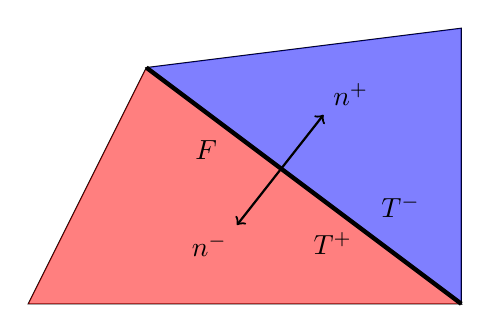
\begin{tikzpicture}[scale=1]
\coordinate (A) at (-1.5, -0);
\coordinate (C) at (0,3);
\coordinate (B) at (4,0);
\coordinate (D) at (4,3.5);

\draw (A) -- (B) -- (C) -- cycle;
\draw (B) -- (C) -- (D) -- cycle;
\fill[red, opacity=0.5] (A) -- (B) -- (C);
\fill[blue, opacity=0.5] (B) -- (C) -- (D);
\draw[ultra  thick] (C) -- (B);

\coordinate (Tm) at (3.6,1.5);
\coordinate (Tp) at (2.0, 0.5);
\coordinate (e) at (0.5, 2.2);
\node[below left] at (Tm) {$T^{-} $ };
\node[above right] at (Tp) {$T^{+}$ };
\node[below right] at (e) {$F$ };

\coordinate (start) at (1.7, 1.7);
\coordinate (endPlus) at (2.25, 2.4);
\coordinate (endMinus) at (1.15, 1.0);

\draw [->, thick] (start) -- (endPlus);
\node[above right] at (endPlus) {$n^{+}$};

\draw [->, thick] (start) -- (endMinus);
\node[below left] at (endMinus) {$n^{-}$};

\end{tikzpicture}

\caption{Facet $F \in \mathcal{F}_h^{int} $ shared by the triangles $T^{+}, T^{-} \in \mathcal{T}_{h} $ and the normal unit vector $n^{+}$ and $n^{-}$. If we pick $T=T^{+}$ and want to evaluate the normal vector $n$ along a facet $F$, then we define $n = n  \mid _{F} = n^{+}$.}
    \label{fig:normal}
\end{figure}



\subsection{Broken Sobolev spaces}%
\label{sub:broken_sobolev_spaces}

In this work will we compute norms on discontinuous elements, thus, it will be necessary to define broken Sobolev spaces.
Let $\mathcal{T}_{h} $ be a mesh and some integer $m\le n$. Then we define the broken Sobolev space to be \[
    \begin{split}
H^{m}( \mathcal{T}_{h} ) & := \left\{ v \in L^2( \Omega )  \mid \ v|_{T} \in H^{m}( T) \quad     \forall T \in  \mathcal{T}_{h} \right\}\\
        L^{2}( \mathcal{F}_{h} ) &:= \left\{ v \in L^2( \mathcal{T}_{h}  )  \mid   \ v|_{F} \in L^{2}( F)  \quad  \forall F \in  \mathcal{F}_{h}   \right\}.
    \end{split}
\]
This motivates us to define broken Sobolev norms and inner products using summation over mesh elements,
\[
 \| v \|_{H^{m}( \mathcal{T}_{h} ) }^{2} = \sum_{T \in  \mathcal{T}_{h} }^{} \| v  \|_{ H^{m}( T ) }^{2  } \quad \text{ and } \quad
 (v ,w )_{H^{m}( \mathcal{T}_{h} ) }^{} = \sum_{T \in \mathcal{T} _{h}}^{} (v ,w )_{ H^{m}( T ) }^{  } .
\]
As before, we use the shorthand notation,  $\| v \|_{\mathcal{T}_{h}} =  \| v \|_{L^{2}( \mathcal{T}_{h} ) }$ and  $(v ,w )_{ \mathcal{T}_{h} }^{} = (v ,w )_{L^2( \mathcal{T}_{h} ) }^{} $.
That is,
\[
 \| v \|_{L^{2}( \mathcal{F}_{h} ) }^{2} = \sum_{F \in  \mathcal{F}_{h} }^{} \| v  \|_{ L^{2}( F ) }^{2  } \quad \text{ and } \quad
 (v ,w )_{L^{2}( \mathcal{F}_{h} ) }^{} = \sum_{T \in \mathcal{F} _{h}}^{} (v ,w )_{ L^{2}( F ) }^{  } .
\]
Again, we often use the more compact notation $\| v \|_{\mathcal{F}_{h}} =  \| v \|_{L^{2}( \mathcal{F}_{h} ) }$ and  $(v ,w )_{ \mathcal{F}_{h} }^{} = (v ,w )_{L^2( \mathcal{F}_{h} ) }^{} $.
A very useful lemma when working with estimates on broken Sobolev spaces is that a if a function is continuous, then the jump between the mesh elements is zero. A function $ v \in  H^{1}( \mathcal{T}_{h} ) $ belongs to $ H^{1}( \Omega )  $ if and only
if $ \jump{ v }   = 0 \text{ for }  F \in \mathcal{F}^{int}_{h}$.

We may denote some the general useful inequalities.
\begin{enumerate}[label=(\roman*)]
    \item A fundamental property of the inner-product the so-called Cauchy-Schwarz inequality
        \begin{equation}
            \label{eq:cauchy-schwartz}
     ( u,v)_{H^{m}( \Omega )  }   \le \| u \|_{H^{m}( \Omega )   }^{  } \| v \|_{H^{m}( \Omega )    }^{  }\quad  \forall u,v \in H^{m}( \Omega )
        \end{equation}

    \item For all  $u \in L ^{2}( \mathcal{T} _{h})$ we have,
\begin{equation}
    \label{eq:mean_jump_estimate}
    \begin{split}
        \| \jump{  u }   \|_{ \mathcal{F} _{h} }^{  } & \le \|  u^{+}   \|_{ \mathcal{F} _{h} }^{  } +
        \| u^{-}   \|_{ \mathcal{F} _{h} }^{  }  \lesssim  \| u \|_{ \partial\mathcal{T }_{h}  }^{2  },\\
        \| \mean{ u }   \|_{ \mathcal{F} _{h} }^{  } & \le \| u^{+} \|_{ \mathcal{F} _{h}  }^{  } + \| u^{-} \|_{ \mathcal{F} _{h}  }^{  }    \lesssim  \| u \|_{ \partial\mathcal{T }_{h}  }^{2  }.
    \end{split}
\end{equation}

    \item For any $a,b >\mathbb{R} $ the well known Young's $\varepsilon $-inequality is on the form,
        \begin{equation}
            \label{eq:young-epsilon}
            2ab \le \varepsilon a^2+ \frac{1}{\varepsilon } b^2.
        \end{equation}

\end{enumerate}



% \begin{enumerate}[label=(\roman*)]
%     \item General inverse inequality.
%     Let $\alpha = ( \alpha _{1}, \ldots, \alpha _{N}) $ and $\beta = ( \beta _{1}, \ldots, \beta _{N} ) $.
%     Assume $u \in H^{\abs{ \beta  }  }( T) $. The following inverse inequalities hold.
%     \[
%         \begin{split}
%         \| \partial ^{\alpha } u \|_{T  }^{  } & \lesssim h^{ - \abs{ \beta  }  } \| \partial ^{\alpha - \beta } u \|_{T }^{  } \\
%         \| \partial ^{\alpha }_{n} u  \|_{F  }^{  } &\lesssim h^{-\frac{1}{2}  } \| \partial ^{\alpha } u \|_{T }^{  }
%         \end{split}
%     \]
% \end{enumerate}
    % For a full triangle we have \[
    % \| v \|_{ \partial T }^{  } \lesssim h_{T}^{-\frac{1}{2}} \| v \|_{ T }^{  } + h_{T}^{\frac{1}{2}} \| \nabla v \|_{ T }^{  }
    % \]




\subsection{Lax-Milgram lemma}%
\label{sub:lax_milgram_lemma}

The intention is to introduce a abstract framework which can handle various types of partial differential equations (PDE). Let  $\mathcal{A} : X \to Y $ be a abstract linear operator encoding the structure of any linear PDE, including boundary
conditions and $X,Y$ are spaces of functions. Then we denote the abstract strong formulation as the equation
\begin{equation}
\label{eq:strong_abs}
\mathcal{A} u = f.
\end{equation}
Where the function $f: \Omega \subset \mathbb{R}^d \mapsto \mathbb{R}$. We assume that the function $u: \Omega \rightarrow \mathbb{R}$ satisfies the relation \eqref{eq:strong_abs} pointwise so that $\mathcal{A} u(x)=f(x) \forall x \in \Omega$.
We will discover that Sobolev spaces are specifically engineered to study these kinds of problems.

\begin{definition}[Linear bounded functional]
    \label{def:linear_function}
Let $V$ be a Hilbert space. Furthermore, we define the dual space $V' $ to be the space of linear and bounded functionals $F: V  \mapsto \mathbb{R} $, i.e., \[
V'  = \left\{ F: V \to \mathbb{R}   \mid  F \text{ is linear and bounded} \right\}
\]
\end{definition}

\begin{problem}[Abstract linear problem]
    \label{def:abstract_linear_problem}
    Assume $X$ and $Y$  to be two Hilbert spaces. Let the vector space $\mathcal{L}( X,Y)  $ be all linear bounded operators spanned from $V$ to $Y$. We define the abstract linear problem as follows; find $u \in V$ s.t. \[
    a( u,v)  = l(v ) := \left<f,v \right>_{V' , V}  \forall v \in V
    \]
    Where $a \in  \mathcal{L} ( V, V,\mathbb{R} ) $ is a bounded bilinear form and $f \in V':= \mathcal{L} ( V,\mathbb{R} )  $ is a bounded linear form associated with the abstract strong formulation \eqref{eq:strong_abs}. Here we denote by $\left<\cdot ,\cdot  \right>_{V',V} $ the duality pairing between $V'$ and $V$.

\end{problem}


\begin{definition}[Coercivity and Boundedness]
    \label{def:coercivity}
    Let $V$ be a Hilbert space and let $a( \cdot ,\cdot )  \in  \mathcal{L} ( V, V,\mathbb{R} )  $. Recall that the bilinear form $a( \cdot ,\cdot ) $ is coercive if \[
     a( v,v) \gtrsim  \| v \|_{ V }^{  } \quad  \forall v \in  V.
    \]
     The bilinear form $a( \cdot ,\cdot ) $ is said to bounded if   \[
    a( u,v)  \lesssim  \| u \|_{ V }^{  }  \| v \|_{V }^{  }\quad  \forall u,v \in V.
    \]
\end{definition}


\begin{lemma}[Lax-Milgram]
    \label{def:lax-milgram}
    The abstract linear problem \ref{def:abstract_linear_problem} is well-posed if $a(\cdot , \cdot  ) $ is bounded and coercive. Moreover, the following a priori estimate holds true.\[
    \| v \|_{ V }^{  } \lesssim  \| f \|_{ V'  }^{  }
    \]
\end{lemma}
\begin{proof}
    The problem can easily be proved using a special case of the Banach–Nečas–Babuška theorem. See \cite[Lemma 1.4]{pietro2012}
\end{proof}



\subsection{Finite element method}%
\label{sub:finite_element_method}


The finite element method (FEM) is a numerical method to solve partial differential equation by finding an approximation of the Problem \ref{def:abstract_linear_problem}.  Let $V_{h}$ be a finite-dimensional (polynomial) approximation space on the mesh
$\mathcal{T} _{h}$. We say that a method is conform if $V_{h}\subset V $ and non-conform if $V _{h} \not\subset V$. We define the approximate problem as follows.
\begin{problem}[The approximate problem]
    \label{def:approx_problem}
    Let $V_{h} \not\subset V$ a non-conform finite-dimensional space. Find  $u_{h} \in V_{h}$ such that, \[
    a_{h}(u_{h},v ) = l_{h}( v) :=  \left<f,v \right>   \forall v \in V_{h}.
    \]
\end{problem}

We denote the functional $a_{h}: V_{h} \times V_{h} \to \mathbb{R} $ as an consistent approximation of $a: V \times V \to \mathbb{R} $, and similarly for the right-hand side $l_{h} : \times _{h} \to \mathbb{R} $ as an approximation of $l: V \to \mathbb{R} $.

\begin{definition}[Local polynomial space]
    \label{def:local_space}
    Let $T$ be a element in a mesh $\mathcal{T}_{h} $,  $x = \left[ x_{1}, \ldots, x_{d} \right] $ be a vector, and $\alpha  = \left[ \alpha _{1}, \ldots, \alpha _{d} \right] \in \mathbb{N} ^{d} $ be a multi index.
    The local polynomial space $\mathcal{P} ^{k}( T) $ for a simplex is denoted as
    \begin{equation}
    \label{eq:pol_space}
        \mathcal{P}^{k}( T) =  \mathrm{span}\left\{ x^{\alpha } \ \text{for } x \in T \text{ and } 0 \le  \alpha _{i} \le k \right\}.
    \end{equation}
    where  $x^{\alpha }$ is a monomial such that $x^{\alpha } = x_{1}^{\alpha _{1}} \ldots x_{d}^{\alpha _{d}}$.

    Let $T$ be a cuboid, i.e.,  $T = \prod_{i=1}^{d} [z_{i}^{-},z_{i}^{+}]$ where $z_{i}^{-}< z_{i}^{+}$ for $z_{i}^{\pm} \in \mathbb{R} $. Then the polynomial space $\mathcal{Q}^{k}( T)$  in $\mathbb{R} ^{d}$ is defined as the tensor product of 1-dimensional
    finite elements, i.e.,
      \[
    \mathcal{Q} ^{k}(T)  := \mathcal{P}^{k}( [z_{1}^{-},z_{1}^{+}] ) \otimes \ldots \otimes \mathcal{P}^{k}( [z_{d}^{-},z_{d}^{+}] )
    \]
\end{definition}
For more information about the local polynomial spaces, see \cite[Chapter 6.4, 7.3]{ErnGuermond2021}

Following Ciarlet \cite[pp.93]{ciarlet1991basic}, the abstract definition of a finite element is defined as the triplet $( T, \mathcal{P}, \Sigma ) $.
In our case, $T$ represents either a simplex or a quadrilateral geometry, and $\mathcal{P}$ denotes a finite-dimensional polynomial space consisting of $N$ shape functions $\left\{ \phi_{i} \right\}_{i\in \mathcal{I} } $, where $\mathcal{I} = \left\{
1, \ldots, N \right\} $, as depicted in Definition \ref{def:local_space}.
On the other hand, $\Sigma $ is the so-called dual of $\mathcal{P}$, that is, the set of linear forms $\left\{ \sigma _{i} \right\}_{i \in \mathcal{I} } $ such that. $ \sigma_{j} ( \phi_{i} ) = \delta _{ij}$ and $p( x) = \sum_{i\in \mathcal{I} }^{} \sigma_{i} ( p) p_{i} $.
If there is a set of points $\left\{ a_{i} \right\}_{i \in \mathcal{I} } $  in $T$ such that
$\sigma_{i}( p) = p( a_{i}) \  \forall p \in \mathcal{P}$,  then the triple $( T, \mathcal{P}, \Sigma  ) $ is called a Lagrangian finite element. The set of points $\left\{ a_{i} \right\}_{i \in \mathcal{I} }  $ is called nodes and is associated with the
so-called nodal basis of $\mathcal{P} $ such that  $\phi ( a_{i}) = \delta _{ij} \ \forall i,j  \in \mathcal{I} $

As anticipated, the local node configuration of the polynomial space is influenced by the form of $T$. For the purpose of our discussion, let us represent the polynomial basis for a simplicial element and a quadrilateral
element as $\mathcal{P} ^{k}(T )$ and $\mathcal{Q} ^{k}( T)$, both of polynomial order $k$. In Figure \ref{fig:ill_nodes} is it illustrated for  $k=1,2,3$ in dimension $d=2$ on how the node configuration evolve.

\begin{figure}[h!]
    \centering
    \hfill
    \subfloat[$\mathcal{P}^{1}( T)  $]{
        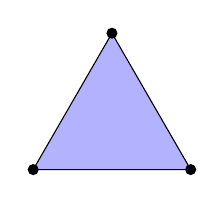
\begin{tikzpicture}[scale=1.0]
            % Define the coordinates
            \coordinate (A) at (0,0);
            \coordinate (B) at (2,0);
            \coordinate (C) at (1,{sqrt(3)});

            % Draw the triangle
            \fill[blue!30] (A) -- (B) -- (C) -- cycle;
            \draw (A) -- (B) -- (C) -- cycle;

            % Draw the nodes
            \fill (A) circle (2pt);
            \fill (B) circle (2pt);
            \fill (C) circle (2pt);
        \end{tikzpicture}
    }
    \hfill
    \subfloat[ $\mathcal{P}^{2}( T)  $]{
        \begin{tikzpicture}[scale=1.0]
            % Define the coordinates
            \coordinate (A) at (0,0);
            \coordinate (B) at (2,0);
            \coordinate (C) at (1,{sqrt(3)});

            % Define the midpoints
            \coordinate (D) at ($(A)!0.5!(B)$);
            \coordinate (E) at ($(B)!0.5!(C)$);
            \coordinate (F) at ($(A)!0.5!(C)$);

            % Draw the triangle
            \fill[blue!30] (A) -- (B) -- (C) -- cycle;
            \draw (A) -- (B) -- (C) -- cycle;

            % Draw the nodes
            \fill (A) circle (2pt);
            \fill (B) circle (2pt);
            \fill (C) circle (2pt);
            \fill (D) circle (2pt);
            \fill (E) circle (2pt);
            \fill (F) circle (2pt);
        \end{tikzpicture}
    }
    \hfill
    \subfloat[$\mathcal{P} ^{3}( T)  $ ]{
        \begin{tikzpicture}[scale=1.0]
            % Define the coordinates
            \coordinate (A) at (0,0);
            \coordinate (B) at (2,0);
            \coordinate (C) at (1,{sqrt(3)});

            % Define the additional points along the edges
            \coordinate (D) at ($(A)!0.3333!(B)$);
            \coordinate (E) at ($(B)!0.3333!(C)$);
            \coordinate (F) at ($(C)!0.3333!(A)$);
            \coordinate (G) at ($(A)!0.6667!(B)$);
            \coordinate (H) at ($(B)!0.6667!(C)$);
            \coordinate (I) at ($(C)!0.6667!(A)$);

            % Define the centroid
            \coordinate (J) at (1, {sqrt(3)/3});

            % Draw the triangle
            \fill[blue!30] (A) -- (B) -- (C) -- cycle;
            \draw (A) -- (B) -- (C) -- cycle;

            % Draw the nodes
            \fill (A) circle (2pt);
            \fill (B) circle (2pt);
            \fill (C) circle (2pt);
            \fill (D) circle (2pt);
            \fill (E) circle (2pt);
            \fill (F) circle (2pt);
            \fill (G) circle (2pt);
            \fill (H) circle (2pt);
            \fill (I) circle (2pt);
            \fill (J) circle (2pt);
        \end{tikzpicture}
    }
    \\
    \hfill
    \subfloat[$\mathcal{Q}^{1}( T)  $]{
        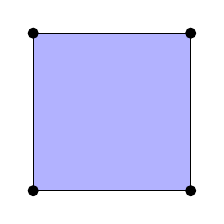
\begin{tikzpicture}[scale=1.0]
            % Define the coordinates
            \coordinate (A) at (0,0);
            \coordinate (B) at (2,0);
            \coordinate (C) at (2,2);
            \coordinate (D) at (0,2);

            % Draw the square
            \fill[blue!30] (A) -- (B) -- (C) -- (D) -- cycle;
            \draw (A) -- (B) -- (C) -- (D) -- cycle;

            % Draw the nodes
            \fill (A) circle (2pt);
            \fill (B) circle (2pt);
            \fill (C) circle (2pt);
            \fill (D) circle (2pt);
        \end{tikzpicture}
    }
    \hfill
    \subfloat[ $\mathcal{Q} ^{2}( T)  $]{
        \begin{tikzpicture}[scale=1.0]
            % Define the coordinates
            \coordinate (A) at (0,0);
            \coordinate (B) at (2,0);
            \coordinate (C) at (2,2);
            \coordinate (D) at (0,2);

            % Define the midpoints
            \coordinate (E) at ($(A)!0.5!(B)$);
            \coordinate (F) at ($(B)!0.5!(C)$);
            \coordinate (G) at ($(C)!0.5!(D)$);
            \coordinate (H) at ($(D)!0.5!(A)$);
            % Define the centroid
            \coordinate (M) at (1, 1);

            % Draw the square
            \fill[blue!30] (A) -- (B) -- (C) -- (D) -- cycle;
            \draw (A) -- (B) -- (C) -- (D) -- cycle;

            % Draw the nodes
            \fill (A) circle (2pt);
            \fill (B) circle (2pt);
            \fill (C) circle (2pt);
            \fill (D) circle (2pt);
            \fill (E) circle (2pt);
            \fill (F) circle (2pt);
            \fill (G) circle (2pt);
            \fill (H) circle (2pt);
            \fill (M) circle (2pt);
        \end{tikzpicture}
    }
    % And so on for $\mathcal{P}^{3}( S)  $, $\mathcal{P}^{4}( S)  $, etc.
    \hfill
    \subfloat[ $\mathcal{Q} ^{3}( T)  $]{
        \begin{tikzpicture}[scale=1.0]
            % Define the coordinates
            \coordinate (A) at (0,0);
            \coordinate (B) at (2,0);
            \coordinate (C) at (2,2);
            \coordinate (D) at (0,2);

            % Define the additional points along the edges
            \coordinate (E) at ($(A)!0.3333!(B)$);
            \coordinate (F) at ($(B)!0.3333!(C)$);
            \coordinate (G) at ($(C)!0.3333!(D)$);
            \coordinate (H) at ($(D)!0.3333!(A)$);
            \coordinate (I) at ($(A)!0.6667!(B)$);
            \coordinate (J) at ($(B)!0.6667!(C)$);
            \coordinate (K) at ($(C)!0.6667!(D)$);
            \coordinate (L) at ($(D)!0.6667!(A)$);

            % Define the internal nodes
            \coordinate (M) at ($(E)+(0,0.6667)$);
            \coordinate (N) at ($(E)+(0,1.332)$);
            \coordinate (O) at ($(I)+(0,0.6667)$);
            \coordinate (P) at ($(I)+(0,1.332)$);

            % Draw the square
            \fill[blue!30] (A) -- (B) -- (C) -- (D) -- cycle;
            \draw (A) -- (B) -- (C) -- (D) -- cycle;

            % Draw the nodes
            \fill (A) circle (2pt);
            \fill (B) circle (2pt);
            \fill (C) circle (2pt);
            \fill (D) circle (2pt);
            \fill (E) circle (2pt);
            \fill (F) circle (2pt);
            \fill (G) circle (2pt);
            \fill (H) circle (2pt);
            \fill (I) circle (2pt);
            \fill (J) circle (2pt);
            \fill (K) circle (2pt);
            \fill (L) circle (2pt);
            \fill (M) circle (2pt);
            \fill (N) circle (2pt);
            \fill (O) circle (2pt);
            \fill (P) circle (2pt);
        \end{tikzpicture}
        }
        \caption{Illustration of the nodes for the element of a simplex a quadrilateral for dimension $d=2$ for polynomial orders $k=1,2,3$.}
        \label{fig:ill_nodes}
\end{figure}


We may introduce the reference element $\hat{T} $ in $d$ dimensions. The reference for a quadrilateral is denoted as $\hat{T} = [0,1]^{d}$. The reference for a simplex in  is defined by the convex hull spanned by the points $( z_{0}, e_{1}, \ldots, e_{d}) $ where $z_{0}:=0$ is the origin and $ \left\{ e_{i}
\right\}_{i=1}^{d} $ is the standard Cartesian  unit basis in $ \mathbb{R} ^{d} $. A corresponding reference finite element is defined as $( \hat{T}, \hat{\mathcal{P} }, \hat{\Sigma}   ) $.



\begin{figure}[th!]
    \centering
    \hspace{-2.2cm}  % Adjust the space as necessary
    \subfloat[]{
        \begin{tikzpicture}[scale=1.0]
            % Define the Reference triange
            \coordinate (A) at (0,0);
            \coordinate (B) at (1,0);
            \coordinate (C) at (0,1);
            \coordinate (G1) at (1/3,1/3);

            \fill[red!30] (A) -- (B) -- (C) -- cycle;
            \draw (A) -- (B) -- (C) -- cycle;
            \fill (A) circle (2pt);
            \fill (B) circle (2pt);
            \fill (C) circle (2pt);

            % Define the arbitary triange
            \coordinate (D) at (2,0);
            \coordinate (E) at (4,0);
            \coordinate (F) at (3,{sqrt(2)});
            \coordinate (G2) at (3, {sqrt(3)/3});

            \fill[blue!30] (D) -- (E) -- (F) -- cycle;
            \draw (D) -- (E) -- (F) -- cycle;
            \fill (D) circle (2pt);
            \fill (E) circle (2pt);
            \fill (F) circle (2pt);

            % Draw arrow to signify the mapping G
            \draw[->, thick, >=stealth] ($(G1)+(0.2,0.2)$) to[bend left] node[midway, above, yshift=0.1cm] {$\mathcal{G}$} ($(G2)+(-0.2,0.2)$);
        \end{tikzpicture}
    }
    \hspace{2.0cm}  % Adjust the space as necessary
    \subfloat[]{
        \begin{tikzpicture}[scale=1.0]
            % Define the Reference quadrilateral
            \coordinate (A) at (0,0);
            \coordinate (B) at (1,0);
            \coordinate (C) at (1,1);
            \coordinate (D) at (0,1);
            \coordinate (G1) at (0.5,0.5);

            \fill[red!30] (A) -- (B) -- (C) -- (D) -- cycle;
            \draw (A) -- (B) -- (C) -- (D) -- cycle;
            \fill (A) circle (2pt);
            \fill (B) circle (2pt);
            \fill (C) circle (2pt);
            \fill (D) circle (2pt);

            % Define the arbitrary quadrilateral
            \coordinate (E) at (2,0);
            \coordinate (F) at (3,1);
            \coordinate (G) at (3,2);
            \coordinate (H) at (2,1);
            \coordinate (G2) at (2.5,0.5);

            \fill[blue!30] (E) -- (F) -- (G) -- (H) -- cycle;
            \draw (E) -- (F) -- (G) -- (H) -- cycle;
            \fill (E) circle (2pt);
            \fill (F) circle (2pt);
            \fill (G) circle (2pt);
            \fill (H) circle (2pt);

            % Draw arrow to signify the mapping G
            \draw[->, thick, >=stealth] ($(G1)+(0.3,0.1)$) to[bend left] node[midway, above, yshift=0.1cm] {$\mathcal{G}$} ($(G2)+(-0.2,0.2)$);
        \end{tikzpicture}
    }
    \\
    \subfloat[]{
        \begin{tikzpicture}[scale=1.0]
            % Define the Reference tetra
            \coordinate (A) at (0,0);
            \coordinate (B) at (1,0);
            \coordinate (C) at (0,1);
            \coordinate (D) at (0.7,0.7);
            \coordinate (G1) at (1/3,1/3);

            \fill[red!65] (A) -- (B) -- (C) -- cycle;
            \fill[red!30] (D) -- (B) -- (C) -- cycle;
            \draw (A) -- (B) -- (C) -- cycle;
            \draw (D) -- (B) -- (C) -- cycle;
            \draw[dashed] (A) -- (D);
            \fill (A) circle (2pt);
            \fill (B) circle (2pt);
            \fill (C) circle (2pt);
            \fill (D) circle (2pt);


            % Define the Translated tetra
            \coordinate (A') at ($(A) + (2,0)$);
            \coordinate (B') at ($(B) + (2,0)$);
            \coordinate (C') at ($(C) + (2.6, 0.6)$);
            \coordinate (D') at ($(D) + (2.5, 0.2)$);

            \fill[blue!65] (A') -- (B') -- (C') -- cycle;
            \fill[blue!30] (D') -- (B') -- (C') -- cycle;
            \draw (A') -- (B') -- (C') -- cycle;
            \draw (D') -- (B') -- (C') -- cycle;
            \draw[dashed] (A') -- (D');
            \fill (A') circle (2pt);
            \fill (B') circle (2pt);
            \fill (C') circle (2pt);
            \fill (D') circle (2pt);

            % Draw arrow to signify the mapping G
            \draw[->, thick, >=stealth] ($(G1)+(0.6,0.2)$) to[bend left] node[midway, above, yshift=0.1cm] {$\mathcal{G}$} ($(D')+(-0.6,0.1)$);
        \end{tikzpicture}
    }
    \hspace{2cm}  % Adjust the space as necessary
    \subfloat[]{
        \begin{tikzpicture}[scale=1.0]
    % Define the Reference cube
    \coordinate (A) at (0,0);
    \coordinate (B) at (1,0);
    \coordinate (C) at (1,1);
    \coordinate (D) at (0,1);
    \coordinate (E) at (0.3,0.3);
    \coordinate (F) at (1.3,0.3);
    \coordinate (G) at (1.3,1.3);
    \coordinate (H) at (0.3,1.3);

    \fill[red!65] (A) -- (B) -- (C) -- (D) -- cycle;
    \fill[red!45] (D) -- (H) -- (G) -- (C) -- cycle;
    \fill[red!30] (B) -- (C) -- (G) -- (F) -- cycle;
    \draw (A) -- (B) -- (C) -- (D) -- cycle;
    \draw (A) -- (E) -- (F) -- (B);
    \draw (D) -- (H) -- (G) -- (C);
    \draw[dashed] (E) -- (H);
    \draw[dashed] (F) -- (G);

    % Define the Translated cube
    \coordinate (A') at ($(A) + (3.3, 0.0)$);
    \coordinate (B') at ($(B) + (3.3, 0.0)$);
    \coordinate (C') at ($(C) + (3.3, 0.0)$);
    \coordinate (D') at ($(D) + (3.3, 0.0)$);
    \coordinate (E') at ($(E) + (2.2, 0.3)$);
    \coordinate (F') at ($(F) + (2.2, 0.3)$);
    \coordinate (G') at ($(G) + (2.2, 0.3)$);
    \coordinate (H') at ($(H) + (2.2, 0.3)$);

    \fill[blue!65] (A') -- (B') -- (C') -- (D') -- cycle;
    \fill[blue!30] (D') -- (H') -- (G') -- (C') -- cycle;
    \fill[blue!45] (D') -- (A') -- (E') -- (H') -- cycle;
    \draw (A') -- (B') -- (C') -- (D') -- cycle;
    \draw (A') -- (E') -- (F') -- (B');
    \draw (D') -- (H') -- (G') -- (C');
    \draw[dashed] (E') -- (H');
    \draw[dashed] (F') -- (G');

    \fill (A') circle (2pt);
    \fill (B') circle (2pt);
    \fill (C') circle (2pt);
    \fill (D') circle (2pt);
    \fill (E') circle (2pt);
    \fill [opacity=0.5] (F') circle (2pt);
    \fill (G') circle (2pt);
    \fill (H') circle (2pt);

    \fill (A) circle (2pt);
    \fill (B) circle (2pt);
    \fill (C) circle (2pt);
    \fill (D) circle (2pt); % D has half opacity now
    \fill [opacity=0.5](E) circle (2pt);
    \fill (F) circle (2pt);
    \fill (G) circle (2pt);
    \fill (H) circle (2pt);

    % Draw arrow to signify the mapping G
    \draw[->, thick, >=stealth] ($(A)+(0.8,0.5)$) to[bend left] node[midway, above, yshift=0.1cm] {$\mathcal{G}$} ($(A')+(-0.5,0.8)$);
\end{tikzpicture}
    }
    \caption{Illustration of affine mapping $\mathcal{G} : \hat{T} \to T $ in dimensions $d=2,3$ from a reference element $\hat{T}$  to element $T$ for simplexes and and quadrilaterals.  } \label{fig:affine_mapping}
\end{figure}

Let the mapping $\mathcal{G} : \hat{T} \to  T$ an affine
mapping, i.e. $\mathcal{G}(x) = Ax +
b$.
The important property of affine transformations is the preservation of parallelism. Hence,  for any two vectors $x,y \in  \hat{T}$ that are parallel in the reference element, their images $\mathcal{G}(x)  $  and $\mathcal{G}( y)  $ will
also be parallel. Generally speaking, an affine transformation of the reference simplex is a transformation to any another simplex of the same dimension. However, for any quadrilateral, an affine transformation preserves the parallelism of opposite
sides, for an illustration see Figure \ref{fig:affine_mapping} and for a counter example see Figure \ref{fig:nonaffine}.

\begin{figure}[h!]
    \centering
    \hspace{-2.2cm}  % Adjust the space as necessary
    \subfloat[]{
        \begin{tikzpicture}[scale=1.0]
            % Define the Reference quadrilateral
            \coordinate (A) at (0,0);
            \coordinate (B) at (1,0);
            \coordinate (C) at (1,1);
            \coordinate (D) at (0,1);
            \coordinate (G1) at (0.5,0.5);

            \fill[red!30] (A) -- (B) -- (C) -- (D) -- cycle;
            \draw (A) -- (B) -- (C) -- (D) -- cycle;
            \fill (A) circle (2pt);
            \fill (B) circle (2pt);
            \fill (C) circle (2pt);
            \fill (D) circle (2pt);

            % Define the arbitrary quadrilateral
            \coordinate (E) at (2,0);
            \coordinate (F) at (3,0);
            \coordinate (G) at (3.5,1);
            \coordinate (H) at (2.5,1);
            \coordinate (G2) at (2.5,0.5);

            \fill[blue!30] (E) -- (F) -- (G) -- (H) -- cycle;
            \draw (E) -- (F) -- (G) -- (H) -- cycle;
            \fill (E) circle (2pt);
            \fill (F) circle (2pt);
            \fill (G) circle (2pt);
            \fill (H) circle (2pt);

            % Draw arrow to signify the mapping G
            \draw[->, thick, >=stealth] ($(G1)+(0.3,0.1)$) to[bend left] node[midway, above, yshift=0.1cm] {$\mathcal{G}$} ($(G2)+(-0.2,0.2)$);
        \end{tikzpicture}
    }
    \hspace{2.0cm}  % Adjust the space as necessary
    \subfloat[]{
        \begin{tikzpicture}[scale=1.0]
            % Define the Reference quadrilateral
            \coordinate (A) at (0,0);
            \coordinate (B) at (1,0);
            \coordinate (C) at (1,1);
            \coordinate (D) at (0,1);
            \coordinate (G1) at (0.5,0.5);

            \coordinate (R1) at (1.5,0.7);
            \coordinate (R2) at (1.4,1.0);

            \fill[red!30] (A) -- (B) -- (C) -- (D) -- cycle;
            \draw (A) -- (B) -- (C) -- (D) -- cycle;
            \draw[very thick] (R1) -- (R2);
            \fill (A) circle (2pt);
            \fill (B) circle (2pt);
            \fill (C) circle (2pt);
            \fill (D) circle (2pt);

            % Define the arbitrary quadrilateral
            \coordinate (E) at (2,0);
            \coordinate (F) at (3.5,0);
            \coordinate (G) at (3.0,1);
            \coordinate (H) at (2.5,1);
            \coordinate (G2) at (2.5,0.5);

            \fill[blue!30] (E) -- (F) -- (G) -- (H) -- cycle;
            \draw (E) -- (F) -- (G) -- (H) -- cycle;
            \fill (E) circle (2pt);
            \fill (F) circle (2pt);
            \fill (G) circle (2pt);
            \fill (H) circle (2pt);

            % Draw arrow to signify the mapping G
            \draw[->, thick, >=stealth] ($(G1)+(0.3,0.1)$) to[bend left] node[midway, above, yshift=0.1cm] {$\mathcal{G}$} ($(G2)+(-0.2,0.2)$);

        \end{tikzpicture}
    }
    \caption{Illustration of an affine mapping $\mathcal{G}: \hat{T} \mapsto T$  versus a non-affine transformation. The left figure preserves parallel lines before and after the transformation, indicating an affine transformation. However, the right figure does not maintain parallelism, making it a non-affine transformation.}
    \label{fig:nonaffine}
\end{figure}

Following \cite[Example 9.4]{ErnGuermond2021}, the $ ( \hat{T}, \hat{\mathcal{P} }, \hat{\Sigma} ) $ is denoted as the reference finite element associated with the nodes $\left\{ \hat{a}_{i} \right\}_{i\in N} $. Let the mapping $\psi $ be function in $\mathcal{L}( \mathcal{P} ^{k}( T), \mathcal{P} ^{k}(\hat{T}
)  )  $ such that is an isomorphic from  $ \psi : \mathcal{P} ^{k}( T) \to \mathcal{P} ^{k}( \hat{T})   $.  Then $\sigma ( p) = \hat{\sigma }( \psi ( p) ) (a_{i} )  = ( p \circ \mathcal{G} )( \hat{a}_{i})      $ for all $p \in \mathcal{P}^{k}( T)  $.
Then the Lagrange interpolation follows,  \[
    p (x) = \sum_{i \in N }^{} \sigma ( a_{i}) \phi_{i}( x) \quad \text{for } a_{i} = \mathcal{G}( \hat{a}_{i}) \quad  \forall i \in N     .
\]
Hence, the finite element $( T, \mathcal{P}, \Sigma  ) $, associated with the notes $\left\{ a_{i} \right\}_{i\in N} $, is reconstructed via the reference finite element $( \hat{T}, \hat{\mathcal{P} }, \hat{\Sigma} ) $.
Thus, using the affine transformation can the definition of the local polynomial space be extended to dependent on the reference element. That is, \[
    \begin{split}
\mathcal{P}^{k}( T) & = \left\{ \hat{v} \circ  \mathcal{G}^{-1}( T)   \mid  \hat{v} \in \mathcal{P}^{k}( \hat{T})      \right\} \\
\mathcal{Q}^{k}( T) & = \left\{ \hat{v} \circ  \mathcal{G}^{-1}( T)     \mid  \hat{v} \in \mathcal{Q}^{k}( \hat{T})      \right\} \\
    \end{split}
\]
Working on shape-regular and affine geometries has shown to greatly simplify and generalise local interpolation estimates, see \cite[Theorem 11.12]{ErnGuermond2021}, and thus is very useful for deriving a priori estimates.
Please note that workarounds exist for proving nonaffine local interpolation estimates, but they require key assumptions on the relationship between the nodes $a_{i}$ and the regularity of the mapping $\mathcal{G} $ \cite[Chapter 13]{ErnGuermond2021}.
Hence, affine meshes is essential for the error analysis which utilize the interpolation estimates, but it limits us to work on structure mesh if we specifically choose on quadrilateral meshes.

\begin{definition}[Broken polynomial spaces]
    Let $\mathcal{T}_{h} $ be a mesh of $\Omega \in \mathbb{R} ^{d} $ and $\Omega _{h} = \bigcup_{T \in \mathcal{T}_{h} } T$ . Let $\mathcal{P}^{k}(T) $ be the space of all polynomials of order $k$ in the mesh element $T$ in $\mathcal{T}_{h}$ . We define the broken polynomial space and the global $C^{0}$ continuous polynomial space as
    \begin{equation}
        \begin{split}
    \mathcal{P}^{k} ( \mathcal{T}_{h} ) & := \left\{ v \in L^{2}( \Omega _{h} )    \mid  v|_{T} \in \mathcal{P}^k( T) \quad  \forall T \in  \mathcal{T}_{h}   \right\}. \\
    \mathcal{P}^{k}_{c} ( \mathcal{T}_{h} ) & := \left\{ v \in C^{0}( \Omega _{h}  )   \mid  v|_{T} \in \mathcal{P}^k( T) \quad  \forall T \in  \mathcal{T}_{h}   \right\}.
        \end{split}
    \end{equation}
    Similarly, for quadrilatural elements is the polynomial spaces defined as,
    \begin{equation}
        \begin{split}
    \mathcal{Q}^{k} ( \mathcal{T}_{h} ) & := \left\{ v \in L^{2}( \Omega _{h} )    \mid  v|_{T} \in \mathcal{Q}^k( T) \quad  \forall T \in  \mathcal{T}_{h}   \right\}. \\
    \mathcal{Q}^{k}_{c} ( \mathcal{T}_{h} ) & := \left\{ v \in C^{0}( \Omega _{h} )   \mid  v|_{T} \in \mathcal{Q}^k( T) \quad  \forall T \in  \mathcal{T}_{h}   \right\}.
        \end{split}
    \end{equation}

\end{definition}

In this thesis will we generally utilize the global $C^{0}$ continuity, hence, for the rest of the thesis do we define
\begin{equation}
    \label{def:Vh_background}
V_{h} =  \left\{ P_{c}^{k}( \mathcal{T}_{h} ) \text{ or }  Q_{c}^{k}( \mathcal{T}_{h} )
 \right\} \end{equation}
Hence, all results holds for both polynomial spaces.

We now have a well-defined discrete global space  $V_{h} $ consisting of the finite set of basis functions $\left\{ \phi _{i} \right\}_{i=1}^{N} $ associated with the Lagriangian nodes $\left\{ a_{i} \right\}_{i=1}^{N}  $. The degree of freedoms,
also known as ndofs, is denoted as $dim(V_{h}) = N$. Let $U_{j} = u_{h}\left(
a_{j} \right) $, so that $u_{h} = \sum_{j=1}^{N} U_{j} \phi _{j}  $. Then the Problem \ref{def:approx_problem} is equivalent to
 \[
\sum_{j = 1}^{N} u_{j} a_{h}\left( \phi _{j}, \phi _{i} \right)  = l_{h}\left( \phi _{i} \right)
\]
Hence, by letting $U = \left[ U_{j} \right] $ , $F = \left[ \left( f, \phi _{i}  \right) _{\Omega } \right] $  and $A = \left[ a_{h}\left( \phi _{j}, \phi _{i} \right)  \right] $ can we construct a linear system,
\begin{equation}
\label{eq:linear_system}
    A U =F.
\end{equation}
Ultimately, the matrix $A$ is shown to be symmetric positive definite only if $a_{h}( \cdot ,\cdot ) $ is well-posed.

\begin{figure}[h!]
\centering
\begin{tikzpicture}[node distance=2cm,
                    box1/.style={rectangle, minimum width=3cm, minimum height=1cm, text centered, draw=black, fill=red!30},
                    box2/.style={rectangle, minimum width=3cm, minimum height=1cm, text centered, draw=black, fill=orange!30},
                    box3/.style={rectangle, minimum width=3cm, minimum height=1cm, text centered, draw=black, fill=green!30},
                    box4/.style={rectangle, minimum width=3cm, minimum height=1cm, text centered, draw=black, fill=blue!30},
                    arrow/.style={thick,->,>=stealth}
                    ]
\node (sf) [box1] {Find $u \in V$ such that $\mathcal{A} u = f$};
\node[left=0.5cm of sf,font=\bfseries, align=right] {Strong formulation:};

\node (alp) [box2, below of=sf] {Find $u \in V$ such that $a(u,v) = l(v) \  \forall v \in V$};
\node[left=0.5cm of alp,font=\bfseries, align=right] {Abstract weak problem:};

\node (dlp) [box3, below of=alp] {Find $u_h \in V_{h}$ such that $a_{h}(u_h,v_h) = l_h(v) \  \forall v_h \in V_{h}$};
\node[left=0.5cm of dlp,font=\bfseries, align=right] {Discrete weak problem:};

\node (lse) [box4, below of=dlp] {Solve $A U = F$};
\node[left=0.5cm of lse,font=\bfseries, align=right] {Linear system of equations:};

\draw [arrow] (sf) -- (alp);
\draw [arrow] (alp) -- (dlp);
\draw [arrow] (dlp) -- (lse);
\end{tikzpicture}
\caption{Workflow of solving linear PDEs using the FEM method.}
\label{fig:fem_workflow}
\end{figure}

To summarize the workflow of solving linear PDEs using the FEM method, see Figure \ref{fig:fem_workflow}.

\subsection{Condition number}%
\label{sub:note_on_condition_number}

Recall the discrete $l^{p}$ norm for a vector,

 \begin{equation}
     \forall U \in \mathbb{R} ^{N}, \quad
\| U  \|_{ p }^{  } =
     \begin{cases}
     &  \left( \sum_{i=1}^{N}  \abs{ U_{i}  }^{p} \right)^{\frac{1}{p}} , \quad  1\le p < \infty \\
   &  \max_{i}  \abs{ U_i },  \quad  p= \infty
     \end{cases}
 \end{equation}
Also recall the definition of the matrix norm,
\begin{equation}
 \forall A \in \mathbb{R} ^{N\times N}, 1\le p \le  \infty, \quad  \| A  \|_{p  }^{  }  = \max_{U \in \mathbb{R} ^{N} \setminus 0} \frac{\| AU \|_{ p }^{  } }{\| U \|_{p}^{  } }.
\end{equation}
Remark that this notation is not to be confused with Sobolev norms.
Assume that $A $ is invertible, then we define the condition number for a matrix in $l^{p}  $ norm defined such that
\begin{equation}
    \label{eq:condition_num}
 \forall A \in \mathbb{R} ^{N\times N}, 1\le p \le  \infty, \quad  \kappa_{p} ( A) = \| A  \|_{ p }^{  } \| A ^{-1} \|_{ p }.
\end{equation}

From basic theory is it known that $\| A \|_{ 2 }^{  } $   is equal to the maximum singular value of $A$ , where singular values of $ A$  are the square roots of the eigenvalues of $A^TA$ \cite[Theorem 2.9]{ suli2003introduction}. Because of the connection
between $\| A \|_{ 2 }^{  } $ norms and its singular values, is $k_{2}( A) $ is often in preferred numerical analysis.
A challenge is that the computations generally involves performing Singular Value Decomposition (SVD)
 or power iteration, which can be quite expensive operations particularly for large sparse matrices.
 However,  $\| A \|_{ \infty }^{  } $ is computed as the maximum absolute row sum and ,hence, only necessary to compute the sum for the non-zero elements in each row. Thus, we seek to estimate
 $\kappa_{2}( A) $ using $ \kappa _{\infty}( A) $.

It is well established that $ \frac{1}{\sqrt{N} }  \| A \|_{ \infty }^{  }  \le \| A \|_{2  }^{  } \le
\sqrt{N}  \| A \|_{\infty  }^{  }  $ for any matrix $A \in R^{N\times N}$  \footnote{
    The identity naturally appears from the standard inequality $\| v \|_{ \infty }^{  } \le  \| v \|_{2  }^{  } \le \sqrt{N}  \| v \|_{ \infty }^{  }   $ for $v \in R^{N}$, which simply comes from the fact that  $ \| v \|_{\infty  }^{ 2 } = \max_{i} \abs{ v_{i} }^{2} \le \sum_{i}^{n}   \abs{ v_{i} }^{2} = \| v \|_{ 2 }^{2  } \le N      \max_{i} \abs{ v_{i} }^{2} = N \| v \|_{
    \infty}^{ 2 }$. Now let $A\in \mathbb{R} ^{N \times N}$ be any matrix. We can then deduce that $ \| A \|_{ 2 }^{  } = \max_{v \in \mathbb{R} ^{N}} \frac{\| Av \|_{2  }^{  }}{\| v \|_{ 2 }^{  } } \ge \max_{v \in \mathbb{R} ^{N}}
    \frac{\| Av \|_{ \infty  }^{  }}{ \sqrt{N} \| v \|_{ \infty}^{  } } = \frac{1}{ \sqrt{N} } \| A \|_{ \infty }^{  }    $ and $ \| A \|_{ 2 }^{  } = \max_{v \in \mathbb{R} ^{N}} \frac{\| Av \|_{2  }^{  }}{\| v \|_{ 2 }^{  } } \le  \max_{v \in \mathbb{R} ^{N}}
    \frac{\sqrt{N} \| Av \|_{ \infty  }^{  }}{  \| v \|_{ \infty}^{  } } =  \sqrt{N} \| A \|_{ \infty }^{  }    $. Hence, the identity $\frac{1}{\sqrt{N} } \| A \|_{\infty  }^{  } \le \| A \|_{ 2 }^{  }\le \sqrt{N} \| A \|_{ \infty  }^{  }   $  is proven.

}. Applying this identity, we obtain the upper and lower bounds for $\kappa_{2}(A)$. Specifically, we have
\begin{equation}
\frac{1}{N} \kappa_{\infty} ( A) \le  \kappa_{2} ( A) \le N \kappa _{\infty}(A)
\end{equation}
Thus, since these norms are equivalent, will we in this thesis focus on $ \kappa_{\infty}( A)  $ because of the efficiency of computing $\| A \|_{ \infty }^{  } $  .

\subsection{Cléments interpolation}%
\label{ssub:clement_operator}
Our goal is to to utilize interpolation estimates to compute convergence rates. An important tool in the process is the so-called Cléments interpolation operator, $C_{h}$.
It is used for interpolation on non smooth functions by applying an regularization on so-called macroelements. However, we need to define affine operations on so-called macroelements before we can proceed with the error estimates.

A patch for a element $\omega \left( T \right) $ is denoted as the set of elements in $\mathcal{T} _{h}$  sharing at least one vertex with $T \in \mathcal{T} _{h}$. Similarly,  a patch of a facet $\omega \left( F \right) $ is defined as the set of all elements in $\mathcal{T}_{h} $
sharing at least one vertex with $F \in  \mathcal{F} _{h}$. For an illustrative example of patches in a two-dimensional triangular mesh, please refer to Figure \ref{fig:example_patch}.

\begin{figure}[ht!]
    \centering

  \centering
    \subfloat{{
    \begin{minipage}[b]{0.45\textwidth}
        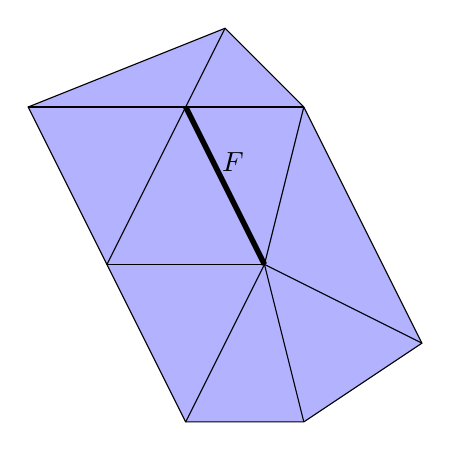
\begin{tikzpicture}
            % Define the coordinates
            \coordinate (A) at (0,0);
            \coordinate (B) at (2,0);
            \coordinate (C) at (1,2);
            \coordinate (D) at (2.5,2);
            \coordinate (F) at (1.5,3);
            \coordinate (E) at (-1,2);
            \coordinate (G) at (1,-2);
            \coordinate (H) at (2.5,-2);
            \coordinate (I) at (4,-1);

            \fill[blue!30] (A) -- (G)-- (H) -- (I)  -- (D) -- (F)-- (E)   -- cycle;

            % Draw the triangle
            \draw (A) -- (G)-- (H) -- (I)  -- (D) -- (F)-- (E)   -- cycle;
            \draw (A) -- (C);
            \draw (A) -- (B);
            \draw (G) -- (B);
            \draw (I) -- (B);
            \draw (F) -- (C);
            \draw (H) -- (B);
            \draw (D) -- (C);
            \draw (D) -- (B);
            \draw (E) -- (C);
            \draw[line width=2pt] (B) -- (C);
            \node at (1.6,1.3) {$F$};

        \end{tikzpicture}
    \end{minipage}\hfill

}}%
    \qquad
    \subfloat{{

    \begin{minipage}[b]{0.45\textwidth}
        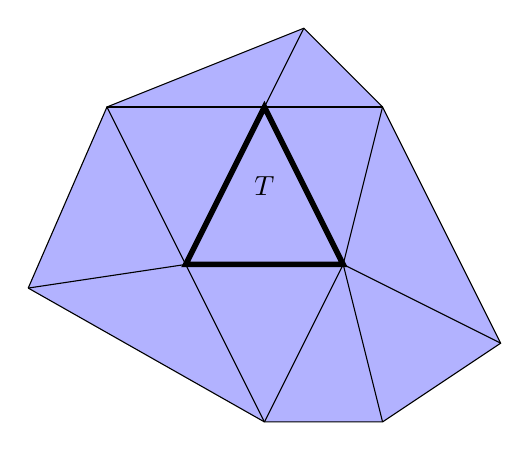
\begin{tikzpicture}
                    % Define the coordinates
        \coordinate (A) at (0,0);
        \coordinate (B) at (2,0);
        \coordinate (C) at (1,2);
        \coordinate (D) at (2.5,2);
        \coordinate (F) at (1.5,3);
        \coordinate (E) at (-1,2);
        \coordinate (G) at (1,-2);
        \coordinate (H) at (2.5,-2);
        \coordinate (I) at (4,-1);
        \coordinate (K) at (-2,-0.3);

        \fill[blue!30] (K) -- (G)-- (H) -- (I)  -- (D) -- (F)-- (E)   -- cycle;
        % \fill[red!30] (B) -- (C) -- (A);

        % Draw the triangle
        \draw (A) -- (G)-- (H) -- (I)  -- (D) -- (F)-- (E)   -- cycle;
        \draw (A) -- (C);
        \draw (A) -- (B);
        \draw (G) -- (B);
        \draw (I) -- (B);
        \draw (F) -- (C);
        \draw (H) -- (B);
        \draw (D) -- (C);
        \draw (D) -- (B);
        \draw (E) -- (C);
        \draw (K) -- (A);
        \draw (K) -- (G);
        \draw (K) -- (E);
        \draw[line width=2pt] (B) -- (C) -- (A) -- cycle;
        \node at (1.0,1.0) {$T$};

        \end{tikzpicture}
    \end{minipage}

    }}%
\caption{Illustration of the patch $\omega ( F) $ on the left-hand side and $\omega(T)$ on the right-hand side.}
    \label{fig:example_patch}%
\end{figure}

\begin{figure}[]
\begin{minipage}{.5\linewidth}
\centering
\subfloat[]{
    \label{fig:macroelements:a}
    \begin{tikzpicture}[scale=0.5]
        % Arbitrary triangle
        \coordinate (A1) at (0,0);
        \coordinate (B1) at (4,1);
        \coordinate (C1) at (1,3);
        \fill [blue!30] (A1) -- (B1) -- (C1) -- cycle;
        \draw (A1) -- (B1) -- (C1) -- cycle;

        % Centroid
        \coordinate (ai) at (barycentric cs:A1=1,B1=1,C1=1);
        \fill (ai) circle (2pt);
        \node[anchor=north east] at (ai) {$a_i$};

        % Reference triangle
        \coordinate (A2) at ($(A1) + (6, 0)$);
        \coordinate (B2) at ($(A2) + (0, 3)$);
        \coordinate (C2) at ($(A2) + (3, 0)$);
        \fill [red!30] (A2) -- (B2) -- (C2) -- cycle;
        \draw (A2) -- (B2) -- (C2) -- cycle;

        % Centroid of the reference triangle
        \coordinate (ahi) at (barycentric cs:A2=1,B2=1,C2=1);
        \fill (ahi) circle (2pt);
        \node[anchor=north west, xshift=-0.1cm, yshift=0.1cm] at (ahi) {$\hat{a}_{j( i)} $};

        \draw[->, thick, >=stealth] ($(ahi)+(0.2,+0.2)$) to[bend right] node[midway, above] {$\mathcal{G}_{A_i}$} ($(ai)+(0.2,+0.3)$);

    \end{tikzpicture}
}
\end{minipage}%
\begin{minipage}{.5\linewidth}
\centering
\subfloat[]{
    \label{fig:macroelements:b}
    \begin{tikzpicture}[scale=0.5]
    % Arbitrary square
    \coordinate (A1) at (0,0);
    \coordinate (B1) at (3,1);
    \coordinate (C1) at (4,4);
    \coordinate (D1) at (1,3);
    \fill[blue!30] (A1) -- (B1) -- (C1) -- (D1) -- cycle;
    \draw (A1) -- (B1) -- (C1) -- (D1) -- cycle;

    % Draw edge from D1 to B1
    \draw (D1) -- (B1);

    % Pick a point on the edge and label it as a_i
    \coordinate (a_i) at ($(D1)!.6!(B1)$);
    \fill (a_i) circle (2pt);
    \node[anchor=north] at (a_i) {$a_i$};

    % Reference equilateral triangle
    \coordinate (A2) at ($(A1) + (6, 0)$);
    \coordinate (B2) at ($(A2) + (2, 3.464)$); % 3.464 = 2 * sqrt(3)
    \coordinate (C2) at ($(A2) + (4, 0)$);
    \fill[red!30] (A2) -- (B2) -- (C2) -- cycle;
    \draw (A2) -- (B2) -- (C2) -- cycle;

    % Divide the equilateral triangle into two right triangles
    \coordinate (M) at ($(A2)!.5!(C2)$);
    \draw (B2) -- (M);

    % Pick a point on the shared edge and label it as ahat_i
    \coordinate (ahat_i) at ($(B2)!.7!(M)$);
    \fill (ahat_i) circle (2pt);
    \node[anchor=north west] at (ahat_i) {$\hat{a}_{j( i)} $};

    % Draw the mapping G_{A_i} from ahat_i to a_i
    \draw[->, thick, >=stealth] ($(ahat_i)+(0.2,0.2)$) to[bend right] node[midway, above] {$\mathcal{G}_{A_i}$} ($(a_i)+(0.2,0.2)$);
\end{tikzpicture}
}
\end{minipage}\par\medskip
\centering
\subfloat[]{
    \label{fig:macroelements:c}
 \begin{tikzpicture}[scale=0.5]

    % Central vertex a_i
    \coordinate (ah_i) at (0, 0);

    % Reference hexagon
    \foreach \angle in {0, 60, ..., 300} {
        \coordinate (A) at (\angle:2.5);
        \coordinate (B) at (\angle + 60:2.5);
        \fill[red!30] (ah_i) -- (A) -- (B) -- cycle;
        \draw (ah_i) -- (A) -- (B) -- cycle;
    }

    \fill (ah_i) circle (2pt);
    \node[anchor=east, yshift=0.25cm] at (ah_i) {$\hat{a}_{j( i) }$};

    \coordinate (A1) at (5, 0);
    \coordinate (B1) at (8, 0);
    \coordinate (C1) at (8, 3);
    \coordinate (D1) at (7, 4);
    \coordinate (E1) at (3.5, 4);
    \coordinate (F1) at (3, 2);
    \fill[blue!30] (A1) -- (B1) -- (C1) -- (D1) -- (E1) -- (F1) -- cycle;
    \draw (A1) -- (B1) -- (C1) -- (D1) -- (E1) -- (F1) -- cycle;

    \coordinate (ai) at (barycentric cs:A1=1,B1=1,C1=1,D1=1,E1=1,F1=1);
    % Draw lines from vertices to a_i
    \draw (A1) -- (ai);
    \draw (B1) -- (ai);
    \draw (C1) -- (ai);
    \draw (D1) -- (ai);
    \draw (E1) -- (ai);
    \draw (F1) -- (ai);
    % Centroid
    \fill (ai) circle (2pt);
    \node[anchor=south, yshift=0.2cm] at (ai) {$a_i$};

    \draw[->, thick, >=stealth] ($(ah_i)+(0.2,- 0.2)$) to[bend right] node[midway, above, yshift=0.1cm] {$\mathcal{G}_{A_i}$} ($(ai)+(-0.2,-0.2)$);

\end{tikzpicture}
}

\caption{Illustration of the different cases when mapping from the reference macroelement $\widehat{A}_{j( i) }$  to the domain $A_{i}$,  $\mathcal{G} _{A_{i}}: \widehat{A}_{j( i) } \to A_{i}$. Here we have defined $\hat{a}_{j(i)} \in
    \widehat{A}_{j(i)}$ s.t. $\mathcal{G}_{A_{i}} ( \hat{a}_{j( i) }) = a_i$. }

\label{fig:macroelements}
\end{figure}


 Let the set  $\left\{ a_{i}\right\}_{i\in N}$ be all Lagrange nodes on the mesh $\mathcal{T}_{h}$. Associated with each node $a_{i}$ we denote the macroelement $A_{i}$ to consist of all elements containing $a_{i}$. Let $n_{cf}$ be the number of configurations for the macroelement, then we define the index $j:
\left\{ 1,\ldots,N \right\} \to \left\{ 1, \ldots, n_{cf} \right\}  $ s.t. $j( i) $ is the index associated with the reference configuration $\widehat{A}_{j(i) }$ for corresponding macroelement $A_{i}$.
Let us define a $C^{0}$-diffeomorphism $\mathcal{G}_{A_{i}}:
\widehat{A}_{j( i) } \to A_{i}$ on the reference macroelements such that for all $\hat{T} \in \widehat{A}_{j( i) } $ is the restriction $\mathcal{G} _{A_{i}}|_{ \hat{T} }$ affine. For an illustration of the reference
macroelement $\widehat{A}_{j( i) }$ and how it related to $a_{i}$ , see
Figure \ref{fig:macroelements}.

The Cléments interpolation operator $C_{h}$ is the $L^2$-projection onto the macroelements. That is, given
a reference macroelement $\widehat{A}_{j( i) }$ and a function $\hat{v} \in L^{1}( \widehat{A}_{j( i) })  $, then $\widehat{C}_{j( i) } \hat{v}$  is the unique polynomial in $\mathcal{P}^{k} ( \widehat{A}_{j( i) })  $ s.t. \[
\int_{  \widehat{A}_{j( i) }}^{} ( \widehat{C}_{j( i) } \hat{v} - \hat{v}) p \ dx  = 0 \quad  \forall p \in \mathcal{P}^{k} ( \widehat{A}_{j( i) })
\]
Finally, the Cléments interpolator is defined as the mapping $C_{h} : L^{1}( \Omega )  \to \mathcal{P} ^{k}_{c}(\mathcal{T}_{h}   ) $ such that
\[
C_{h} v = \sum_{i=1}^{N} \widehat{C}_{j( i) } ( v (\mathcal{G} _{A_{i}}) (\mathcal{G}^{-1}_{A_{i}}(a_{i})) )\phi _{i},
\]
where $\phi _{i}$ is the corresponding polynomial basis associated with the node $a_{i}$.

% Recall the general Sobolev norm notation,
% \[
% \| u \|_{ m,p,T }^{  } = \left( \sum_{ \left\lvert \alpha  \right\rvert \le m}^{} \int_{T}^{}  \left\lvert  \partial ^{\alpha } u \right\rvert^{p} dx   \right)^{\frac{1}{2}}
% \]
% where we use the convenient notation $\| u \|_{L^2(T) }^{  } = \| u \|_{ T  }^{  } = \| u \|_{ 0,2,T  }^{  } $ and similarly $\| u \|_{ H^r( T )  }^{  } = \| u \|_{ r,T  }^{  } = \| u \|_{ r,2,T  }^{  }  $.


Finally, we have the following a priori estimate.

\begin{lemma}
    \label{lemma:clements}

    Let $v \in H^{s}( \Omega ) $. We define the Clement interpolation as the mapping
$C_{h}: L^{2}( \Omega )   \to  V_{h}$, where $V_{h}$ has the order $k$. Then does the following stability estimate hold,
\[
 \| C_{h} v \|_{ s, \Omega     }^{  } \lesssim \| v \|_{ s, \Omega   }^{  } \quad \forall v \in H^{s}( \Omega ) ,
\]
Let $r = \mathrm{min} ( s, k+1) $. If the following conditions for an parameter $l$ is satisfied, it exists error estimates such that
\begin{equation}
    \begin{split}
      0\le l \le r  \implies \| v - C_{h} v \|_{ m,T   }^{  }  &  \lesssim h^{r-l}_{T} \| v \|_{l,\omega \left( T \right)  }^{  } \quad  \forall T \in \mathcal{T} _{h}, \forall v \in H^{l}( \omega \left( T \right)
      ), \\
      0\le l \le r-\frac{1}{2}  \implies \| v - C_{h} v \|_{ m,F }^{  } & \lesssim h^{r - l - \frac{1}{2}}_{T} \| v \|_{l,\omega \left( F \right)  }^{  } \quad  \forall \partial T \in \mathcal{T} _{h}, \forall v \in H^{l}( \omega \left( F
      \right)).
    \end{split}
\end{equation}

\end{lemma}


\begin{corollary}
    \label{cor:celement_apriori}
    Let $0 \le l \le k+1$ and let $0\le m \le \min_{} ( 1,l )$.
    Given Lemma \ref{lemma:clements}  then does the following estimate hold
    \[
    \inf_{v_{h} \in V_{h} } \| v - v_{h} \|_{  m,\Omega }^{  } \lesssim  C h^{l-m}  \| v \|_{ l,\Omega  }^{  } \quad     \forall v \in H^{l}( \Omega ).
    \]
\end{corollary}
This result is very useful since it is now sufficient to show that a priori estimates holds to prove convergence rate. For further detailed information about the Cléments interpolation, please investigate \cite[Chapter 1.6]{ern04}.

\subsection{Useful local inverse estimates}%
\label{sub:some_general_inequalities}


    Choose any element $T \in \mathcal{T}_{h} $ and let $v_{h} \in \mathcal{P} ^{m}( T)   $. Then does the local inverse estimate hold,
\begin{equation}
\label{eq:inv1}
\abs{ v_{h} }_{H^{l}( T) }  \lesssim h^{m-l} \abs{ v_{h} }_{H^{m}( T  ) }
\text{ for } l \le m.
\end{equation}
 For proof, see \cite[Lemma 12.1]{ErnGuermond2021}. An essential example is the following inequality.
 \begin{equation}
     \label{eq:degrade}
\| D^2v_{h} \|_{T  }^{  } \lesssim h^{-1} \| \nabla v_{h}  \|_{ T  }^{  } \lesssim h^{-2} \| v_{h} \|_{T  }^{  }
 \end{equation}

Another very useful inequality is the so-called trace inequality which connect the relationship of evaluating the norm on element $ T $ and with any of the corresponding facets $F \in \partial T$. The general form is
\begin{equation}
    \label{eq:inv2}
\| v_{h} \|_{F   }^{  }  \lesssim
h^{-\frac{1}{2}} \| v_{h} \|_{ T  }^{  },
\end{equation}
For proof, see \cite[Lemma 12.8]{ErnGuermond2021}.

Let $\partial _{n} v = \nabla v \ n$ and $\partial_{nn} v = n^{T} D^2 v \ n $. Keeping in mind that the normal vector has a unit length and, thus, evidently applying the
trace inverse inequality we have two present useful examples,
\begin{equation}
    \label{eq:fund_inv_est}
\begin{split}
    \| \partial _{n} v_{h} \|_{F  }^{  }  & \le \| \nabla v_{h} \|_{F  }^{  }  \le h^{-\frac{1}{2}} \| \nabla  v_{h} \|_{T  }^{  },  \\
    \| \partial _{nn} v_{h} \|_{ F }^{  } & \le  \| D^2 v_{h} \|_{ F }^{  }   \le  h^{-\frac{1}{2}} \| D^2 v_{h} \|_{ T }^{  }.
\end{split}
\end{equation}
Combining \eqref{eq:inv1} and \eqref{eq:inv2}, we establish that
\begin{equation}
    \label{eq:general}
\abs{ v_{h} }_{l,F}  \lesssim h^{m-l - \frac{1}{2}} \abs{ v_{h} }_{m, T}
\text{ for } l \le m.
\end{equation}

\subsection{Cea's lemma}%
\label{sub:ceas_lemma}

Assume that we have a discrete bilinear form $a_{h}: X_{h}\times X_{h} \to \mathbb{R} $ and let $X _{h} \subseteq  V $ be the discrete conform polynomial space. We transition the problem to find a solution, $u_{h} \in  \mathcal{V}_{h}$, so it holds that $a\left( u_{h},v_{h} \right)  = l\left( v_{h} \right) \ \  \forall v_{h} \in X _{h} $.
Since the method is conform, i.e., $X _{h} \subseteq  V $, does it exists a exact solution, $u \in  \mathcal{V}$, such that \(
a \left( u, v_{h} \right)  = l\left( v_{h} \right)  \ \  \forall v_{h} \in  X _{h}.
\)
Furthermore, the problem is said to be strongly consistent since it fulfills the Galerkin orthogonality property, that is $ a\left( u -u_{h} , v_{h} \right)  =0$. Thus, if $u_{h},v_{h} \in  X _{h}$, then
\begin{equation}
\label{eq:cealemma_proof}
    \begin{split}
\alpha \| u -u_{h} \|_{ V  }^{ 2 } & \le  a\left( u - u_{h}, u - u_{h}  \right)    \\
&= a\left( u - u_{h}, u -v_{h} \right) - a\left( u -u_{h}, v_{h} - u_{h} \right)  \\
 &  \le  M \| u - u_{h} \|_{ V  }^{  }  \| u - v_{h} \|_{ V  }^{  }
    \end{split}
.\end{equation}
Hence, we now have the so-called Ceas lemma, \[
\| u - u_{h} \|_{ V  }^{  }  \lesssim  \inf_{v_{h} \in X_{h} } \|  v_{h} - u \|_{V  }^{  }.
\]
A useful property is that for a conformal numerical method to converge can we now simply require \[
\lim_{h \to 0}  \inf_{v_{h} \in  X_{h}}  \| v - v_{h} \|_{ V  }^{  } = 0 \quad  \forall v \in V.
\]
In that case will $\| u - u_{h} \|_{ V  }^{  }  \to  0$, $h \to  0$. Hence, if this requirement is fulfilled, the numerical methods will converge to a unique solution.
For more information, see \cite[p. 66]{quartdiff}.

In combination with Corollary \ref{cor:celement_apriori}, is Cea's lemma very handy to construct a priori estimates. However, Ceas lemma as it stands does assume conform methods $X_{h} \subset X$, hence, we must be cautious for broken Sobolev spaces.





    
\section{Continuous interior penalty methods for the biharmonic problem with Cahn-Hilliard type boundary conditions}%
\label{sec:CIP_biharmonic_problem}

One of the objective of this section is to discuss the strong formulation for the biharmonic problem (BH).
Following this, we will present both the continuous weak formulation and the derivation of the two proposed discrete weak formulations, specifically the continuous interior penalty methods.
We then present a short discussion of the current status of the properties of the methods.

\subsection{The biharmonic problem with C-H boundary conditions}%
\label{sub:the_biharmonic_problem_with_c_h_boundary_conditions}

Recall the BH problem.
Let $\Omega \subseteq    \mathbb{R} ^d$ be a bounded polygonal domain and $\Gamma $ be its corresponding boundary. Also let $\mathcal{T}_{h} = \left\{ T \right\} $ be a shape-regular fitted mesh s.t. $\mathcal{T}_{h} = \Omega $. Let the BH problem have the form,
\begin{subequations}
\begin{align}
    \Delta^2  u  + \alpha  u  & = f( x)  \quad \text{in } \Omega,   \label{eq:bi_problem_a}\\
    \partial _{n} u & = g_{1}(x)   \quad \text{on } \Gamma ,  \label{eq:bi_problem_b}\\
    \partial _{n} \Delta  u & = g_{2}( x)   \quad \text{on } \Gamma .  \label{eq:bi_problem_c}
\end{align}
\label{eq:bi_problem}
\end{subequations}
Here is $\Delta ^2 = \Delta  \left( \Delta  \right) $ the biharmonic operator, also known as the bilaplacian. We will assume for the strong form that $u \in H^{4}\left( \Omega  \right) $, $\alpha  >0 $ and $f \in L^{2}\left( \Omega  \right)
$. The functions $g_{1},g_{2}: \Omega  \to \mathbb{R}$ are denoted as boundary conditions similar to the CH problem.

\begin{remark}
It is worth noting that the problem is closely related to the Kirchhoff's plate problem by changing the boundary conditions such that $u = \partial _{n } u = 0$ on $\Gamma $, which is in the literature known as so-called clamped boundary conditions.
Many of the papers we refer to may consider clamped boundary condition and not the CH boundary conditions. The main difference relies on if the problem is treated with homogeneous or non-homogeneous boundary conditions and if the discrete space is
imposing the Dirichlet and Neumann conditions strongly in the discrete solution space or weakly using the Nitsche's method \cite{nitsche1971variationsprinzip}.
\end{remark}

We want to construct a weak form for the strong BH problem \eqref{eq:bi_problem}. Let $v \in H^{2}( \Omega ) $  Using Greens Theorem is it obvious that \(
\left( \Delta ^2 u,v \right) _{ \Omega  }   = ( \partial _{n} \Delta u, v ) _{\Gamma   } - ( \nabla \left( \Delta  u \right) , \nabla v ) _{ \Omega }
\).
Applying a new iteration of the Greens theorem we get
$ -( \nabla ( \Delta u ) , \nabla v ) _{\Omega  }  =   ( \Delta u, \Delta v ) _{\Omega } - ( \Delta u, \partial _{n}v )_{\Gamma } $.
Hence, we obtain the identity
\begin{equation}
\label{eq:iden_bi}
( \Delta ^2 u, v ) _{\Omega } = ( \Delta u, \Delta v)_{\Omega } +  ( \partial _{n} \Delta u, v)_{\Gamma } - ( \partial _{n} v, \Delta u) _{\Gamma }
\end{equation}
Taking into account the boundary conditions, we end up with the following corresponding weak formulation of the biharmonic problem \eqref{eq:bi_problem}.

\begin{equation}
\label{eq:V_deg}
V := \left\{ v \in  H^2( \Omega )  \mid \partial _{n} v  = g_{1}   \right\}
\end{equation}
Consider the bilinear form $a:V\times V \to \mathbb{R}$ and the linear form $l: V \to \mathbb{R}$. We define the continuous weak formulation problem formulation as follows.

Find a $u \in   $ such that
\begin{equation}
\label{eq:cont_weak_problem}
a( u,v) = l( v)  \forall v \in V
\end{equation}
where
\begin{equation}
    \begin{split}
a( u,v) & =  ( \alpha u,v)_{\Omega } + ( \Delta u, \Delta v)_{\Omega } - (  \Delta u, \partial _{n} v) _{\Gamma }\\
l( v)  &= ( f,v)_{\Omega } - ( g_{2} , v)_\Omega
    \end{split}
\end{equation}
Note that the Neumann boundary condition $g_{1}$ is strongly imposed in $V$, and $g_{2}$ is naturally incorporated in the weak formulation.


\subsection{Detailed construction of Hessian and Laplacian Formulations }%
\label{sub:construction_of_laplacian_cip}
The goal is to construct a corresponding discrete version for the problem \eqref{eq:cont_weak_problem}, that is to find a $u_{h} \in V_{h}$ such that $a_{h}( u_{h}, v_{h}) = l_{h}( v_{h}) $ for all $v_{h} \in V_{h}$.

To achieve the objective of constructing the Hessian and Laplacian formulations, the following lemmas will be the primary components. This is done by constructing a consistent formulation by assuming the function $u$ is exact with a sufficient
regularity, and the test function $v_{h}$ defined as an element from the nonconforming set $V_{h} \not\subset V$.
This asserts when we have a bilinear form and replace the exact solution with $u_{h} \in V_{h}$, the system still remains consistent in $V$. However, due to the nonconformal nature of $V_{h}$, it becomes necessary to introduce penalty terms to ensure the system is well-posed. Keep in mind that the $C^{1}$
continuity is imposed weakly and in the same way is the Neumann conditions also imposed weakly.

\subsubsection{Construction of the Hessian formulation}%
\label{ssub:construction_of_the_hessian_formulation}



\begin{lemma}
    Assume the homogeneous Neumann conditions $g_1 = 0 $.
Let $u \in H^{4}( \Omega ) $ be the solution to \eqref{eq:bi_problem} and let $ v \in V_{h}$. Then does the following identity hold.
\begin{equation}
\label{eq:bi_basic_dg_full}
\begin{split}
    \left( \Delta  ^{2} u, v_h \right) _{\Omega }  =&   \left( D^2u, D^2v_h \right)_{\Omega }   -  ( \mean{ \partial _{nn} u }   , \jump{ \partial_{n} v_h } )_{\mathcal{F}_{h}^{int} } -  (  \jump{ \partial_{n} u
    },\mean{ \partial _{nn} v_h } )_{\mathcal{F}_{h}^{int} } \\
    & - ( \partial _{nn} u , \partial _{n} v_h)_{\Gamma  }- ( \partial _{n} u , \partial _{nn} v_h)_{\Gamma  } +  \left(g_{2}, v_h  \right) _{ \Gamma  }
\end{split}
\end{equation}
\end{lemma}

\begin{proof}

 We will start constructing a local theory for a element $T$ and then extend it to the full mesh
$\mathcal{T}_{h} $. Using Greens Theorem is it obvious that
\begin{equation}
    \label{eq:id1}
\left( \Delta ^2 u,v_h \right) _{T }   = \left( \partial _{n} \Delta u, v_h \right) _{\partial T  } - \left( \nabla \left( \Delta  u \right) , \nabla v_h \right) _{T }
\end{equation}

We can expand the second term in the following way.
\begin{equation}
    \label{eq:id2}
    \begin{split}
( \nabla ( \Delta u ) , \nabla v_h ) _{T } & = \sum_{i = 1}^{ d}  ( \Delta  \partial _{x_{i}} u, \partial _{x_{i}}v_h ) _{T }
                                           = \sum_{i = 1}^{d}  ( \nabla \cdot ( \nabla \partial _{x_{i}} u ) , \partial _{x_{i}} v_h )_{T }  \\
&= \sum_{i = 1}^{d}  \left( ( \partial_n  \partial _{x_{i}} u,  \partial _{x_{i}} v_h ) _{\partial T } -   ( \nabla \partial _{x_{i}} u, \nabla \partial _{x_{i}} v_h )_{T } \right) \\
& = (  \partial_n\nabla u, \nabla v_h ) _{\partial_{} T  } - ( D^2 u, D^2v_h ) _{T }
    \end{split}
.\end{equation}
Hence, the normal flux of $\Delta u$ appears naturally into the formulation. It can be denoted that $D^2$ is the Hessian matrix operator. Also remark that we apply the notation
$( D^2u, D^2v_h )_{\Omega } = \int_{\Omega }^{} D^{2}u : D^2v_h  dx$ for the inner product $D^2u:D^2v_h$.

Next, we want to decompose the evaluation of $\partial _{n}\nabla  u $ on the boundary $\partial T$ in the tangential and normal direction. Pick a facet  $F \in \partial T$, then we define the following decomposition of linear transformation $\nabla u = P_{F}\nabla u  + Q_{F}  \nabla u  $ s.t. the
orthogonality, $
P_{F} \nabla u  \cdot Q_{F}  \nabla u = 0$, holds. Here, the normal projection matrix is defined as $Q_{F} = n \otimes n $ and the tangential decomposition follows from $ P_{F} = I - Q_{F} = I - n \otimes n  =  \sum_{i=1}^{d-1} t_{i} \otimes t_i$,
where we defined a orthonormal basis $t_{i}$, $i = 1, \ldots, d-1$ for the space orthogonal to the outer normal vector $n$ on a facet $F$. Let $ a_{1}, a_{2}, a_{3} \in \mathbb{R} ^{d}$ be any vectors, then it is well known that the following identity holds $ ( a_{1}
\otimes a_{2}  ) a_{3} = ( a_{2}^{T}  a_{3}) a_{1} $. Hence, we have
\begin{equation}
\label{eq:projection}
    \begin{split}
   Q_{F} \nabla u & = ( n \otimes n ) \nabla u =  (n^{T} \nabla u)n \\
   P_{F} \nabla u & =( I - n \otimes n ) \nabla u =   \nabla u  - (n^{T}  \nabla u)n =  \sum_{ i =1 }^{d-1} ( t_{i}^{T}  \nabla u ) t_{i}
    \end{split}
\end{equation}

Given that $u$ is evaluated only on $\partial T$ can we write
$\nabla u = \left( n^{T} \nabla u   \right) n + \sum_i^{d-1} \left( t_i^{T} \nabla u   \right) t_i$ such that,
\begin{equation}
\label{eq:id3}
    \begin{split}
(  \partial_n\nabla u, \nabla v_h ) _{\partial_{} T  } & =  ( \partial _{n} ( \partial_{n}u \ n), \partial _{n} v_h \ n )_{\partial T}   +\sum_{i,j=1}^{d-1} ( \partial _{n} ( \partial_{t_{i}}u \ t_{i}), \partial _{t_{j}} v_h \ t_{j} )_{\partial T} \\
& =  ( \partial _{nn} u, \partial _{n} v_h  )_{\partial T}+\sum_{i=1}^{d-1} ( \partial _{n t_{i}}u , \partial _{t_{i}} v_h  )_{\partial T}
    \end{split}
\end{equation}
Here we used that $n^{T} n = 1$ and $t_{i}^{T} t_{j} = \delta_{ij}$.
Remark that simple relation was applied,
    \begin{align*}
\partial_n (\partial_n u)  & = n^T \nabla (\partial_n u)  = n ^T (D^2 u \ n)  = n^{T} D^2 u \ n = \partial _{nn} u, \\
\partial_n (\partial_{t_{i}} u)  & = t_{i}^T \nabla (\partial_n u)  = t_i^T (D^2 u \ n )   = n^{T} D^2 u \ t_{i} = \partial _{n t_{i}} u.
    \end{align*}
We may also deduce the relationship $\partial _{nt_{i}} u = \partial _{t_{i}n}u$ which arise from the fact that $n^{T} D^2u \ t_{i} = ( t_{i}^{T} D^2u \  n)^T = t_{i}^{T}  D^2u \  n$, where we utilized the symmetry $D^2u = ( D^2u) ^{T} $ and that the
product is a scalar.
Combining \eqref{eq:id1}, \eqref{eq:id2} and \eqref{eq:id3} we see that,
\[
    ( \Delta ^2 u, v_h) _{T}   = ( D^2 u, D^2v_h)_{T } + ( \partial _{n}  \Delta u, v_h )_{\partial T} -( \partial _{nn}u ), \partial _{n} v_h  )_{\partial T}-\sum_{i=1}^{d-1} ( \partial _{n t_{i}}u, \partial _{t_{i}} v_h  )_{\partial T}
\]
Since we aim construct a identity for the full mesh $\mathcal{T} _{h}$, we sum over the elements.
\begin{equation}
\label{eq:bi_basic_dg2}
\left( \Delta  ^{2} u,v_h \right) _{\Omega } = \sum_{T \in  \mathcal{T} _{h}}^{}  ( D^2 u, D^2v_h)_{T } + ( \partial _{n}  \Delta u, v_h )_{\partial T} -( \partial _{nn}u , \partial _{n} v_h  )_{\partial T}-\sum_{i=1}^{d-1} ( \partial _{n t_{i}} u , \partial _{t_{i}} v_h  )_{\partial T}
\end{equation}
Our goal is to simplify the equation above so we can take account for discontinuities of the derivatives.
By integrating over exterior facets $\mathcal{F} _{h}^{ext}$ and interior facets $\mathcal{F} _{h}^{int}$ we will get e more suitable formulation which makes it easier to control the jumps between the elements, hence makes it possible to penalize discontinuities.

\begin{equation*}
    \begin{split}
 ( \Delta  ^{2} u,v_h ) _{\Omega }  =&\sum_{T\in \mathcal{T} _{h}}^{} ( D^2u,D^2v_h ) _{T }  + (\partial _{n} \Delta  u,v_h)_{\partial T} - (\partial _{nn} u, \partial _{n}v_h )_{\partial T}  - \sum_{i=1}^{d-1} ( \partial _{t_{i}n}u , \partial _{t_{i}} v_h  )_{\partial T}   \\
= &\sum_{T\in \mathcal{T} _{h}}^{} ( D^2u,D^2v_h ) _{T }  + \sum_{F \in \mathcal{F}_{h}^{ext} }^{}  (\partial _{n} \Delta  u,v_h)_{F} - (\partial _{nn} u, \partial _{n}v_h )_{F}  - \sum_{i=1}^{d-1} ( \partial _{ t_{i}n} u , \partial _{t_{i}} v_h
)_{F}     \\
   &  + \sum_{F \in \mathcal{F} _{h}^{int}}^{} \underbrace{\left( (\partial _{n^{+}} \Delta  u^{+}
        ,v_h^{+} )_{F}
+ \left(\partial _{n^{-}} \Delta  u^{+} ,v_h^{-}\right)_{F}  \right)}_{(I)}    \\
    &\quad \quad  -
\underbrace{\left( \left(\partial _{n^{+}n^{+}} u^{+}, \partial _{n^{+}} v_h^{+} \right) _{F} + \left(\partial _{n^{-}n^{-}} u^{-}, \partial _{n^{-}} v_h^{-}
\right) _{F} \right) }_{(II)} \\
   &  \quad \quad - \sum_{i=1}^{d-1}\underbrace{( (\partial _{n^{+}t_{i}} u^{+}, \partial_{t_{i}} v_h^{+} )_{F} +  \left(\partial _{n^{-}t_{i}} u^{-},
        \partial_{t_{i}} v_h^{-}
\right)_{F} ) }_{(III)} \\
    \end{split}
.\end{equation*}

Where integration of the interior facets is computed in the following fashion.
\begin{equation}
    \label{eq:dg2_facets}
    \begin{split}
        (I) &  =    \left(\partial _{n^{+}} \Delta  u^{+} ,v_h^{+}\right)_{F} +
        \left(\partial _{n^{-}} \Delta  u^{-} ,v_h^{-}\right)_{F}  \\
            & =   \int_{F}^{}
            \jump{ \partial _{n} \Delta  u \cdot v_h } =
            \int_{F}^{}
            \mean{ \partial _{n} \Delta  u } \underbrace{\jump{ v_h }}_{= 0}    + \underbrace{\jump{ \partial _{n} \Delta  u
            }}_{= 0}    \mean{ v_h } = 0 \\
            (II) &  =     \left(\partial _{n^{+}n^{+}} u^{+}, \partial_{n^{+}} v_h^{+} \right)_{F} +  \left(\partial _{n^{-}n^{-}} u^{-}, \partial_{n^{-}} v_h^{-} \right)_{F}    \\
                 &= \int_{F}^{} \jump{ \partial _{nn} u \cdot  \partial_{n} v_h }   = \int_{F}^{}
                       \mean{ \partial _{nn} u    } \underbrace{\jump{ \partial_{n} v_h }  }_{\neq 0}    + \underbrace{\jump{ \partial
                               _{nn}  u
                       }}_{= 0}    \mean{ \partial _{n}v_h } \\
            (III) &  =     \left(\partial _{n^{+}t_{i}} u^{+}, \partial_{t_{i}} v_h^{+}
                \right)_{F} +  \left(\partial _{n^{-}t_{i}} u^{-}, \partial_{t_{i}} v_h^{-}
                \right)_{F}   \\
                 &  =   \int_{F}^{}
                 \jump{ \partial _{nt_{i}} u \cdot  \partial_{t_{i}} v_h } =
                 \int_{F}^{}
                 \mean{ \partial _{nt_{i}} u    } \underbrace{\jump{ \partial_{t_{i}} v_h }  }_{= 0}    + \underbrace{\jump{ \partial
                         _{nt_{i}}  u
                 }}_{= 0}    \mean{ \partial _{t_{i}}v_h }  = 0
                   \end{split}
.\end{equation}
Observe that the cancellations in the term $(I)$ and term $(III)$  appears of the continuity of $v_h\in V_{h} $ and $u\in H^{4}( \Omega ) $ which makes the jumps and derivative jumps zero. On the other hand, the second term $(II)$  does not vanish
since the derivative of $v_h \in V_{h}$ has a nonzero jump. It can also be raised that $\mean{
\partial _{nn} u } = \partial _{nn} u  $ holds of $H^{4}( \Omega  ) $.

Combining \eqref{eq:dg2_facets} and inserting the boundary condition $g_{2} = \partial _{n} \Delta u $ is it clear that the formulation presented in \eqref{eq:bi_basic_dg2} is equivalent to the following formulation.
\begin{equation}
\label{eq:bi_basic_dg_full_1}
\begin{split}
    \left( \Delta  ^{2} u, v_h \right) _{\Omega }  =&   \left( D^2u, D^2v_h \right)_{\mathcal{T} _{h}} +  \left(g_{2}, v_h  \right) _{\Gamma  }  -  ( \mean{ \partial _{nn} u }   , \jump{ \partial_{n} v_h } )_{\mathcal{F}_{h}^{int} } \\
                                                  &  - ( \partial _{nn} u , \partial _{n} v_h)_{\mathcal{F}^{ext}_{h} } - \sum_{i =1  }^{d-1} ( \partial   _{t_{i}n} u  ,  \partial   _{t_{i}}  v_h  )_{ \mathcal{F}^{ext} _{h}  }
\end{split}
\end{equation}
Under the assumption that $g_{1} = 0$ on $\Gamma$, and given that the tangential decomposition is orthogonal to $n$, we can assert that $ \partial_{t_{i} n} u = \partial_{t_{i}} ( \partial _{n} u ) = 0 $ holds for any $i = 1,\ldots, d$. This implies that the
last term of the equation vanish.

We also note that we add consistent symmetry terms $( \mean{ \partial _{nn} v_h } ,\jump{ \partial _{n} u }    )_{\mathcal{F}^{int}_{h} } $ and $( \partial _{nn} v_h  , \partial _{n} u     )_{\Gamma  } $, which effectely is adding zero
because of the regularity of $u$ and the boundary condition $g_{1}=0$. Finally, we have
\begin{equation}
\begin{split}
    \left( \Delta  ^{2} u, v_h \right) _{\Omega }  =&   \left( D^2u, D^2v_h \right)_{\Omega }   -  ( \mean{ \partial _{nn} u }   , \jump{ \partial_{n} v_h } )_{\mathcal{F}_{h}^{int} } -  (  \jump{ \partial_{n} u
    },\mean{ \partial _{nn} v_h } )_{\mathcal{F}_{h}^{int} } \\
    & - ( \partial _{nn} u , \partial _{n} v_h)_{\Gamma  } - (\partial _{nn} v_h , \partial _{n} u)_{\Gamma  } +  \left(g_{2}, v_h  \right) _{ \Gamma  }
\end{split}
\end{equation}

The proof is complete.

\end{proof}

We will now assemble the Hessian CIP formulation. Assume $u,v \in V_{h}$ and $g_{1} = 0$, then we have the linear form
\begin{equation}
    \label{eq:hessian_form}
\begin{split}
a_{h}^{H} \left( u, v \right)   =&
    \left( \alpha  u, v \right) _{\Omega }   +  \left( D^2 u, D^2v \right) _{\Omega } \\
 & - \left( \mean{  \partial _{n n} u }, \jump{ \partial _{n }u} \right)_{\mathcal{F}_{h}^{int}}  -
 \left( \mean{ \partial _{n n} v }, \jump{ \partial _{n}u }      \right)_{\mathcal{F}_{h}^{int}}  + \frac{\gamma }{h}  \left( \jump{ \partial _{n} u}, \jump{ \partial _{n} v   }   \right)_{\mathcal{F}_{h}^{int}} \\
 & - \left(   \partial _{n n} u ,  \partial _{n }v \right)_{\Gamma }  -
 \left( \partial _{n}u , \partial _{n n} v       \right)_{\Gamma }  + \frac{\gamma }{h}  \left(  \partial _{n} u,  \partial _{n} v      \right)_{\Gamma }   \\
 l_{h}^{H}( v)  =&  \left( f, v \right) _{\Omega }  - \left(g_{2}, v  \right) _{\Gamma }
\end{split}
.
\end{equation}

Thus, the Hessian formulation is derived. Note that we added two consistent penalty terms. What we will see later that this term is essential for making the problem well-posed, hence, the name interioir penalty method. For more information of CIP nonconform error analysis, see \cite[Chapter 1.3]{pietro2012}.

\subsubsection{Construction of the Laplacian formulation}%
\label{ssub:construction_of_the_laplacian_formulation}


\begin{lemma}

 Let $u \in H^{4}( \Omega ) $ the solution of \eqref{eq:bi_problem} and $v \in  V_{h}$. Then we have the following identity.
\[
    \begin{split}
( \Delta ^2 u, v ) _{\Omega }  =& ( \Delta u, \Delta v)_{\mathcal{T} _{h} }  +  ( \jump{ \partial _{n} u} , \mean{ \Delta v })_{\mathcal{F}_{h}^{int} }+  (  \mean{ \Delta u }, \jump{ \partial _{n} v} )_{\mathcal{F}_{h}^{int} } \\
& + ( g_{2} , v )_{\Gamma } - ( \partial _{n} v, \Delta u)_{\Gamma }- ( \partial _{n} u, \Delta v)_{\Gamma } +( g_{1} , \Delta v)_{\Gamma } .
    \end{split}
\]
\end{lemma}

\begin{proof}


  Similarly, we start constructing a local theory for a element $T$ and then extend it to the full mesh $\mathcal{T}_{h} $.
Utilizing \eqref{eq:iden_bi} can we construct a local identity s.t. \[
( \Delta ^2 u, v ) _{T} = ( \Delta u, \Delta v) +  ( \partial _{n} \Delta u, v)_{\partial T} - ( \partial _{n} v, \Delta u) _{\partial T}
\]
Now, summing over all elements we get \[
    \begin{split}
( \Delta ^2 u, v ) _{\Omega } & = \sum_{T \in \mathcal{T}_{h} }^{}  ( \Delta u, \Delta v)_{T}
+  ( \partial _{n} \Delta u, v)_{\partial T} - ( \partial _{n} v, \Delta u) _{\partial T} \\
 & =   ( \Delta u, \Delta v)_{\mathcal{T} _{h}} +  \sum_{F \in \mathcal{F}_{h}^{ext} }^{}
  \overbrace{( \partial _{n} \Delta u, v)_{ F}}^{=( g_{2},v)_{F} }  - ( \partial _{n} v, \Delta u) _{F} \\
  &   \quad + \sum_{F \in \mathcal{F}_{h}^{int} }^{} \underbrace{( ( \partial _{n^{+}} \Delta u, v)_{ F} + ( \partial _{n^{-}} \Delta u, v)_{ F} )}_{(I)}  - \underbrace{( ( \partial _{n^{+}} v, \Delta u) _{F} + ( \partial _{n^{-}} v, \Delta u) _{F}
  )}_{(II)}   \\
    \end{split}
\]
Decomposing the terms and utilizing the regularity of $u$ and $v$ is it easy to see that,    \[
\begin{split}
    (I) & = ( \partial _{n^{+}} \Delta u, v)_{ F} + ( \partial _{n^{-}} \Delta u, v)_{ F}  = \int_{F}^{} \left[ \partial _{n} \Delta u \cdot  v \right] =  (  \mean{ \partial _{n^{+}} \Delta u } , \underbrace{\jump{v  }}_{ = 0}      )_{ F} + (  \underbrace{\jump{ \partial _{n}
    \Delta u }}_{=0}  , \mean{v  }     )_{ F} \\
    (II) &=  ( \partial _{n^{+}} v, \Delta u) _{F} + ( \partial _{n^{-}} v, \Delta u) _{F} = \int_{F}^{} \jump{ \partial _{n} v, \Delta u } =  ( \underbrace{\jump{ \partial _{n} v}}_{ \neq 0 } , \mean{ \Delta u })_{F}  + ( \mean{ \partial _{n} v}, \underbrace{\jump{ \Delta u
    }}_{=0} )_{F}
\end{split} .
\]
Hence, we end up with the identity,
\[
( \Delta ^2 u, v ) _{\Omega } = ( \Delta u, \Delta v)_{\mathcal{T} _{h} }  +  ( \jump{ \partial _{n} v} , \mean{ \Delta u })_{\mathcal{F}_{h} }  + ( g_{2} , v )_{\Gamma } - ( \partial _{n} v, \Delta u)_{\Gamma }.
\]

We add consistent symmetry terms $(  \jump{ \partial _{n} u }, \mean{ \Delta  v })_{\mathcal{F}^{int}_{h} } $ and $(  \partial _{n} u, \Delta  v       )_{\Gamma  } -(  g_{1}, \Delta  v  )_{\Gamma  }  $, which effectely is adding zero
because of the regularity of $u$ and boundary condition $\partial _{n} u = g_{1}$.
Adding the terms, we end up with the final formulation,
\[
    \begin{split}
( \Delta ^2 u, v ) _{\Omega }  =& ( \Delta u, \Delta v)_{\mathcal{T} _{h} }  +  ( \jump{ \partial _{n} u} , \mean{ \Delta v })_{\mathcal{F}_{h}^{int} }+  (  \mean{ \Delta u }, \jump{ \partial _{n} v} )_{\mathcal{F}_{h}^{int} } \\
& + ( g_{2} , v )_{\Gamma } - ( \partial _{n} v, \Delta u)_{\Gamma }- ( \partial _{n} u, \Delta v)_{\Gamma } +( g_{1} , \Delta v)_{\Gamma } ,
    \end{split}
\]
and the proof is complete.
\end{proof}

Finally, can we construct the Laplace CIP formulation. Let $u,v \in V_{h}$, then can finally write the following respective forms.

\begin{equation}
    \label{eq:laplace_form}
    \begin{split}
        a_{h}^{L} \left( u, v \right)   =&
        \left( \alpha  u, v \right) _{\Omega }   +  \left( \Delta  u, \Delta v \right) _{ \Omega } \\
                                         & - \left( \mean{  \Delta  u }, \jump{ \partial _{n }v} \right)_{\mathcal{F}_{h}  }  - \left( \mean{ \Delta  v }, \jump{ \partial _{n}u }      \right)_{\mathcal{F}_{h}^{int}  }  + \frac{\gamma }{h}  \left( \jump{ \partial _{n} u}, \jump{ \partial _{n} v   }   \right)_{\mathcal{F}_{h}^{int} } \\
                                         & - \left(   \Delta  u ,  \partial _{n }v \right)_{\Gamma   }  - \left(  \Delta  v ,  \partial _{n}u       \right)_{\Gamma  }  + \frac{\gamma }{h}  \left(  \partial _{n} u,  \partial _{n} v      \right)_{ \Gamma } \\
        l^{L}_{h}( v_{h}) & =  \left( f, v \right) _{\Omega } - ( g_{2},  v )_{\Gamma } -  ( g_{1}, \Delta  v  )_{\Gamma }  + \frac{\gamma }{h} ( g_{1}, \partial _{n} v  )_{\Gamma }
    \end{split}
\end{equation}


In contrast to the Hessian formulation, is the boundary Neumann booundary condition $g_{1}$ is imposed weakly using the Nitsche's method, hence, the regularization term.
This consists of adding a symmetry term and adding an additional stabilization regularisation term \cite{nitsche1971variationsprinzip}.
It is worth noting that technically is the interior regularisation equivalent to do a Nitsche's method in all interior boundaries of the elements with boundary conditions of each element weakly
imposed to zero. Thus, we expect the penalty parameter $\gamma$ to be the same interior and exterior elements. Let where $k\ge 2$ is the polynomial order, then for the Hessian formulation is it theoretically proven that $\gamma = 2k ( k-1 ) $
\cite{brenner2012quadratic, brenner2012}. However, we still prefer to experimentally verify the best parameter.

\subsection{Continuous interior penalty formulations}%
\label{sub:continuous_interior_penalty_formulations}

We define the two CIP formulations associated with biharmonic problem \eqref{eq:bi_problem} following \cite{brenner2012} and \cite{feng2007fully}. The general idea is to utilize the constructed bilinear and linear forms in \eqref{eq:laplace_form} and \eqref{eq:hessian_form} to solve the problem: Find a
$u \in V_{h}$ such that $a_{h}( u, v) = l_{h}( v) $ for all $v \in V_{h}$. To summarize, we have the following formulations.

First, note that since $V_{h} \not\subset V $ is it necessary to define the space $V \oplus V_{h}$, which essentially is the direct sum of these two spaces. This new space includes all elements from $V$ and $V_h$ and all possible linear combinations of these elements. i.e., let $u \in V$ and $u_{h} \in V_{h}$, then $u + u_{h} \in V \oplus V_{h} $.

\begin{enumerate}[label=\arabic*)]
    \item Assuming that $g_{1} = 0$. Then Hessian problem formulation is
\begin{equation}
        \label{eq:cip_hessian_form}
\begin{split}
a_{h}^{H} \left( u, v \right)   =&
    \left( \alpha  u, v \right) _{\Omega }   +  \left( D^2 u, D^2v \right) _{\Omega } \\
 & - \left( \mean{  \partial _{n n} u }, \jump{ \partial _{n }v} \right)_{\mathcal{F}_{h}^{int}}  -
 \left(  \jump{ \partial _{n}u }, \mean{ \partial _{n n} v } \right)_{\mathcal{F}_{h}^{int}}  + \frac{\gamma }{h}  \left( \jump{ \partial _{n} u}, \jump{ \partial _{n} v   }   \right)_{\mathcal{F}_{h}^{int}} \\
 & - \left(   \partial _{n n} u ,  \partial _{n }v \right)_{\Gamma }  -
 \left(    \partial _{n}u,  \partial _{n n} v \right)_{\Gamma }  + \frac{\gamma }{h}  \left(  \partial _{n} u,  \partial _{n} v      \right)_{\Gamma } \\
 l_{h}^{H}( v)  =&  \left( f, v \right) _{\Omega }  - \left(g_{2}, v  \right) _{\Gamma }
\end{split}
.
\end{equation}

With the corresponding energy norms,
\begin{equation}
\label{eq:a_cip_energy_norm_hes}
    \begin{split}
 \| v \|_{ a_{h} }^{ 2 }& = \alpha  \| v\|_{ \Omega  }^{2  }  +  \| D ^2 v \|_{ \Omega   }^{ 2 }  + \|  h^{-\frac{1}{2}} \jump{ \partial _{n} v    }\|_{  \mathcal{F} _{h}^{int} }^{2  }+ \|  h^{-\frac{1}{2}}  \partial _{n} v    \|_{  \Gamma  }^{2  },  \quad v \in V_{h}  \\
   \| v \|_{ a_{h},* }^{ 2 } &= \| v \|_{ a_{h} }^{ 2 }  + \| h^{\frac{1}{2}}  \mean{     \partial _{nn } v}  \|_{ \mathcal{F}_{h}^{int}   }^{  2}+ \| h^{\frac{1}{2}} \partial _{nn } v  \|_{ \Gamma    }^{  2}, \quad  v\in V \oplus V_{h}.
    \end{split}
\end{equation}


\item The Laplace formulation is
    \begin{equation}
        \label{eq:cip_laplace_form}
        \begin{split}
            a_{h}^{L} \left( u, v \right)   =&
            \left( \alpha  u, v \right) _{\Omega }   +  \left( \Delta  u, \Delta v \right) _{ \Omega } \\
                                             & - \left( \mean{  \Delta  u }, \jump{ \partial _{n }v} \right)_{\mathcal{F}_{h}^{int}  }  - \left( \mean{ \Delta  v }, \jump{ \partial _{n}u }      \right)_{\mathcal{F}_{h}^{int}  }  + \frac{\gamma }{h}
                                             \left( \jump{ \partial _{n} u}, \jump{ \partial _{n} v   }   \right)_{\mathcal{F}_{h}^{int} } \\
                                             & - \left(   \Delta  u ,  \partial _{n }v \right)_{\Gamma   }  - \left(  \partial _{n}u,  \Delta  v \right)_{\Gamma  }  + \frac{\gamma }{h}  \left(  \partial _{n} u,  \partial _{n} v      \right)_{ \Gamma } \\
                                             l^{L}_{h}( v)  =&  \left( f, v \right) _{\Omega } - ( g_{2},  v )_{\Gamma } -  ( g_{1}, \Delta  v  )_{\Gamma }  + \frac{\gamma }{h} ( g_{1}, \partial _{n} v  )_{\Gamma }
                                         \end{split}
                                     \end{equation}
                                     With the corresponding energy norms
                                     \begin{equation}
                                         \label{eq:a_cip_energy_norm_lap}
                                         \begin{split}
                                             \| v \|_{ a_{h} }^{ 2 }& = \alpha \| v\|_{ \Omega  }^{2  }  +  \| \Delta   v \|_{ \Omega   }^{ 2 }  + \|  h^{-\frac{1}{2}} \jump{ \partial _{n} v    }\|_{  \mathcal{F} _{h}^{int} }^{2  } +  \|  h^{-\frac{1}{2}}
                                             \partial _{n} v  \|_{  \Gamma  }^{2  },  \quad v \in V_{h}  \\
                                             \| v \|_{ a_{h},* }^{ 2 } &= \| v \|_{ a_{h} }^{ 2 }  + \| h^{\frac{1}{2}}  \mean{     \partial _{nn } v}  \|_{ \mathcal{F}_{h}^{int}   }^{  2}+ \| h^{\frac{1}{2}}       \partial _{nn } v  \|_{ \Gamma    }^{  2}, \quad  v\in V \oplus V_{h}.
                                         \end{split}
                                         .
                                     \end{equation}


\end{enumerate}

\begin{remark}
It should be noted that the Hessian formulation has a substantial limitation in that it is only valid for homogeneous Neumann conditions. This constraint arises from the challenges associated with imposing $g_{1}$ via the tangential derivative terms in Equation \eqref{eq:bi_basic_dg_full_1} during the proof of Lemma \ref{lemma:bh_hessian_identity}.
From a physical perspective, this is not problematic as it aligns with the boundary conditions of the original CH problem \eqref{eq:strongch}. However, from the standpoint of numerical validation, the homogeneous Neumann condition enforces strict
rules on the design of manufactured solutions on arbitrary domains. Consequently, the examples illustrated in section \ref{sec:numerical_results} are only demonstrated on simple domains. This particular constraint does not apply to the Laplace formulation.
\end{remark}

The Hessian formulation is well investigated by Susanne Brenner in several papers for \cite{brenner2012, brenner2012quadratic, brenner2012quadratic_kirk} with a corresponding analysis and numerical validation. Similarly, variants of the Laplace formulation can be found here
\cite{feng2007fully, georgoulis2009discontinuous}. In these article there also is good theoretical and experimental evidence that both formulation have the following expected a priori estimates. Let  $u \in H^{s}( \Omega ) $ for $s\ge  \frac{5}{2} + \varepsilon$, and $u_{h}\in
V_{h}  $ of order $k\ge 2$. Then with $r = \min\left\{ s,
k+2 \right\}$ the a priori estimates are   \[
    \begin{split}
\| u - u_{h} \|_{ a_{h},*  }^{  }  & \lesssim  h^{r-2} \| u \|_{ r, \Omega  }^{  } \\
\| u - u_{h} \|_{ \Omega   }^{  }  & \lesssim  h^{r- \max_{}\left\{ 0, 3-k \right\}  } \| u \|_{ r,\Omega  }^{  }
    \end{split}
\]

Remark that the $\| \cdot  \|_{\Omega   }^{  } $ norm estimates is suboptimal for $k=2$.
\red{Need to clarify assumptions on the boundary. Maybe regularity of $g_{1}$ and $g_{2}$.  }



\subsection{Note on the Biharmonic Mixed Formulation}%
\label{subsec:biharmonic_mixed_formulation}

It is easy to see that the biharmonic problem can be rewritten into an equivalent mixed formulation , that is, to find $\sigma, \tau  \in H^2( \Omega ) $ s.t. \[
    \begin{split}
\Delta \sigma  & = f \quad  \text{in } \Omega \\
\sigma   & = \Delta u  \text{ in } \Omega \\
\partial _{n} \sigma  & = g_{1} \text{ on } \Gamma  \\
\partial _{n} u   & = g_{2} \text{ on } \Gamma
    \end{split}
\]
The goal is to obtain an useful weak formulation. Using Greens theorem on the first equation we get,
\[
( \sigma, v)_{\Omega } = ( \nabla  u , \nabla v  )_{\Omega } - ( \nabla _{n} u , v) _{\Gamma }.
\]
Similarly for the second equation we obtain
\[
( \nabla \sigma , \nabla \varphi  )_{\Omega} - ( \partial _{n} \sigma ,  \varphi )_{\Gamma } = ( f,\varphi ) _{\Omega}
\]
Putting it all together we have the following mixed weak formulation; Find $( u, \sigma ) \in H^{1}( \Omega ) \times H^{1}( \Omega )  $ s.t. \[
    \begin{split}
     ( \nabla  u , \nabla v  )_{\Omega } -( \sigma, v)_{\Omega }  & =   ( g_{1} , v) _{\Gamma } \quad  \forall v \in H^{1}( \Omega ) \\
( \nabla \sigma , \nabla \varphi  )_{\Omega}  & = ( f,\varphi ) _{\Omega} + ( g_{2} ,  \varphi )_{\Gamma } \quad  \forall \varphi \in H^{1}( \Omega )
    \end{split}
\]
Now we want to relate this formulation to the abstract saddle point problem (SPP).
Let $V = H^{1}( \Omega ) $  and $W=H^{1}( \Omega ) $ be  Hilbert spaces and define the bilinear form $a: V\times V \to \mathbb{R}  $ and $b: V \times W \to \mathbb{R} $ s.t. $a( \sigma,v ) = - ( \sigma , v) _{\Omega }  $ and $b( u,v) = ( \nabla u,
\nabla v)_{\Omega  }  $. We also may define the linear forms, $G,F: V \to \mathbb{R} $ s.t. $ G( v)  = ( g_{1}, v) _{\Gamma } $ and $F( \varphi ) = ( f, \varphi )_{\Omega } + ( g_{2}, \varphi )_{\Gamma } $.

Hence, we obtain the following SPP. Find $( u,\sigma ) \in V \times W$ s.t.  \[
    \begin{cases}
       a( \sigma ,v) + b ( u, v )  & = G( v)   \quad  \forall v \in V \\
       b( u, \varphi  )  & = F( \varphi )     \quad \forall \phi \in W
    \end{cases}
\]
This is useful since we can now apply standard saddle point theory to do an analysis for the problem. We will see that it is now easier to handle the boundary constraints naturally, but with the cost of a more challenging time discretization
procedure.
For more information about the biharmonic mixed formulation, see \cite{babuvska1980analysis,cai2023nitsche}.
However, in this master thesis is the focus on solving the biharmonic equation avoiding the mixed formulation using the CIP formulation, which does in fact handle the downsides with the SPP problem.


% A well known and mature application for SPP is the well known Stokes equation, hence, a good place to start \cite{john2016finite, knabner2003numerical}.




    \newpage
\section{Cut continuous interior penalty methods for the biharmonic problem}%
\label{sec:cutcip_biharmonic_problem}


Questions arise when we want to allow for complex geometries where some physical domain $\Omega $ has a smooth boundary $\Gamma $.
A method would be to generate a structured background mesh which fully covers $\Omega $, but does not necessarily fit to the boundary perfectly.
For consistency, integration of the contribution is performed on the physical domain, but the involved discrete test and trial functions in $V_{h}$ are defined on the background mesh.
However, we will run into geometrical problems when
so-called cut finite elements has a very small intersection of the physical domain, i.e, $\abs{ T \cap \Omega  }_{d} \ll \abs{ T }_{d}  \lesssim h^{d}$ and $\abs{ \Gamma \cap T }_{d-1} \ll  h^{d-1}$, where $\abs{\ \cdot \  }_{d} $ is the
measure of the volume in dimension $d$.
The cut elements are identified as a crucial geometric issue since the inverse inequalities outlined in Section \ref{sub:some_general_inequalities} do not generalize well to these elements. This identifies the challenges in establishing theoretical stability and a priori estimates for any geometric arrangement.

One way do handle this issue is to introduce the so-called cut finite element method (CutFEM).
The method involves adding a stabilization term, commonly referred to as the ghost penalty term.
This term serves the purpose of controlling the energy norm associated with the bilinear form, utilizing the entire background mesh to ensure stabilization and geometric robustness.
For more information, see
\cite{burman2015cutfem, burman2010ghost, burman2022cutfem, burman2012fictitious}.
Inspired by the corresponding CutFEM DG elliptic framework outlined in \cite{gurkan2019stabilized}, the objective of this section is to engineer suitable stabilized ghost penalty terms for the biharmonic problem, starting from the CIP methods introduced in Section \ref{sec:CIP_biharmonic_problem}.
We will show what assumptions are needed for the ghost-penalty method for the discrete problem to be stable in Section \ref{sub:stability_estimate} and derive optimal convergence in Section \ref{sec:a_priori_estimates}.  Once
this is fulfilled we propose a ghost penalty which fulfills these assumptions in Subsection \ref{sec:constructing_ghost_penalties}.


\subsection{Computational domain}%
\label{sub:unfitted_mesh}

\begin{figure}[h!]
    \centering
% \subfloat[]{\label{a1}
%         \begin{tikzpicture}[scale=0.7]

%             \draw[fill=blue!30] (0.1, 0.1) circle (1.5cm);
%             % Background mesh
%             \foreach \i in {-2.5, -2, ..., 2.5} {
%                 \draw[line width=0.1pt, shift={(-2.5,\i)}, opacity=0.2] (0,0) -- (5,0);
%                 \draw[line width=0.1pt, shift={(\i,-2.5)}, opacity=0.2] (0,0) -- (0,5);
%             }


%             % Labels
%             \node[below right] at (-0.2,0.4) {$\Omega$};
%             \node[below right] at (1.2,1.5) {$\Gamma$};
%         \end{tikzpicture}

% }\hfill
\subfloat[]{\label{a}
        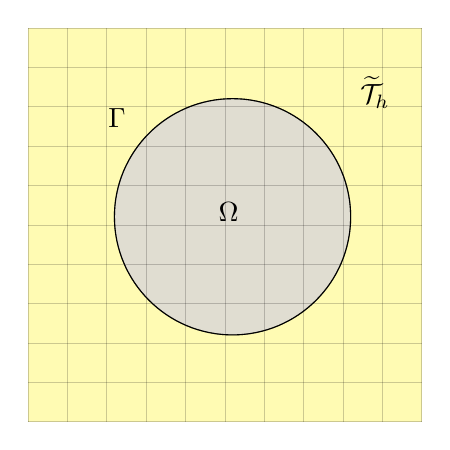
\begin{tikzpicture}[scale=1.0]

            \fill[yellow!30] (-2.5,2.5) -- (2.5,2.5) -- (2.5,-2.5) -- (-2.5,-2.5) -- cycle;
            \draw[fill=blue!30, opacity=0.4] (0.1, 0.1) circle (1.5cm);

            \draw (0.1, 0.1) circle (1.5cm);
            % Background mesh
            \foreach \i in {-2.5, -2, ..., 2.5} {
                \draw[line width=0.1pt, shift={(-2.5,\i)}, opacity=0.2] (0,0) -- (5,0);
                \draw[line width=0.1pt, shift={(\i,-2.5)}, opacity=0.2] (0,0) -- (0,5);
            }

            \node[below right] at (-0.2,0.4) {$\Omega$};
            \node[below right] at (-1.6,1.6) {$\Gamma$};

            % Labels
            \node[below right] at (1.6,2.0) {$\widetilde{\mathcal{T}}_{h}$};
        \end{tikzpicture}

}\hfill
\subfloat[]{\label{c}
        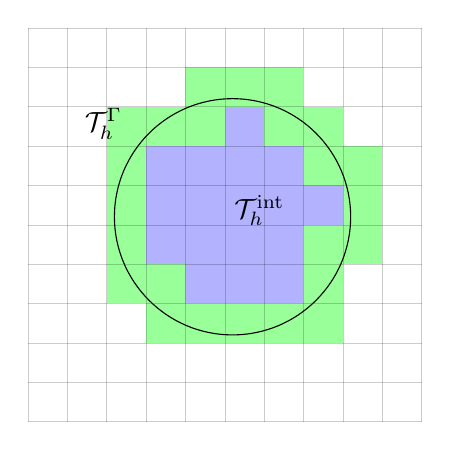
\begin{tikzpicture}[scale=1.0]

            % POTENTIAL ACTIVE MESH
            \fill[blue!30] (2,2) -- (2,-1.5) --(-1.5,-1.5) -- (-1.5,2) -- cycle;

            % ELEMENTS WITH NO INTERSECTION
            % lower left
            \fill[white] (-1.5,-1.5) rectangle (-1.0,-1.0);
            \fill[white] (-1.5,2.0) rectangle (-1.0,1.5);
            \fill[white] (-1.0,2.0) rectangle (-0.5,1.5);
            \fill[white] (2,2) rectangle (1.5,1.5);
            \fill[white] (1.5,2) rectangle (1.0,1.5);
            \fill[white] (2,1.5) rectangle (1.5,1.0);
            \fill[white] (1.5,-1) rectangle (2,-1.5);
            \fill[white] (1.5,-0.5) rectangle (2,-1.0);

            % CUT ELEMENTS
            \fill[green!40] (-0.5,2.0) rectangle (1.0,1.5);
            \fill[green!40] (-1.5,1.5) rectangle (0.0,1.0);
            \fill[green!40] (0.5,1.5) rectangle (1.5,1.0);
            \fill[green!40] (-1.5,1.0) rectangle (-1.0,-1.0);
            \fill[green!40] (-1.0,-0.5) rectangle (-0.5,-1.5);
            \fill[green!40] (-0.5,-1.5) rectangle (1.5,-1.0);
            \fill[green!40] (1.5,-1) rectangle (1.0,-0.0);
            \fill[green!40] (1.5,-0.5) rectangle (2.0,1.0);
            \fill[green!40] (1.0,0.5) rectangle (1.5,1.0);

            \draw (0.1, 0.1) circle (1.5cm);
            % Background mesh
            \foreach \i in {-2.5, -2, ..., 2.5} {
                \draw[line width=0.1pt, shift={(-2.5,\i)}, opacity=0.2] (0,0) -- (5,0);
                \draw[line width=0.1pt, shift={(\i,-2.5)}, opacity=0.2] (0,0) -- (0,5);
            }


            % Labels
            \node[below right] at (0.0,0.5) {$\mathcal{T}^{\mathrm{int} }_{h}$};
            \node[below right] at (-1.9,1.6) {$\mathcal{T}^{\Gamma }_{h}$};
        \end{tikzpicture}
}
\hfill
\subfloat[]{\label{b}
        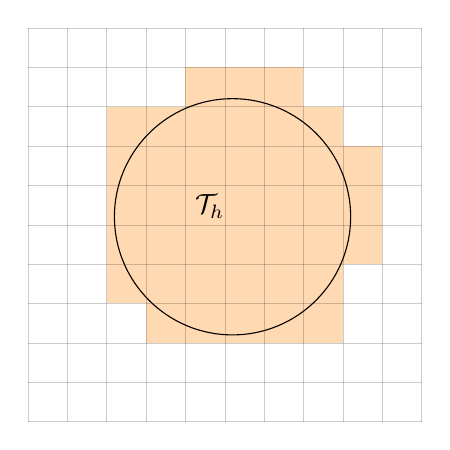
\begin{tikzpicture}[scale=1.0]

            % POTENTIAL ACTIVE MESH
            \fill[orange!30] (2,2) -- (2,-1.5) --(-1.5,-1.5) -- (-1.5,2) -- cycle;

            % ELEMENTS WITH NO INTERSECTION
            % lower left
            \fill[white] (-1.5,-1.5) rectangle (-1.0,-1.0);
            \fill[white] (-1.5,2.0) rectangle (-1.0,1.5);
            \fill[white] (-1.0,2.0) rectangle (-0.5,1.5);
            \fill[white] (2,2) rectangle (1.5,1.5);
            \fill[white] (1.5,2) rectangle (1.0,1.5);
            \fill[white] (2,1.5) rectangle (1.5,1.0);
            \fill[white] (1.5,-1) rectangle (2,-1.5);
            \fill[white] (1.5,-0.5) rectangle (2,-1.0);

            % CUT ELEMENTS
            \fill[orange!30] (-0.5,2.0) rectangle (1.0,1.5);
            \fill[orange!30] (-1.5,1.5) rectangle (0.0,1.0);
            \fill[orange!30] (0.5,1.5) rectangle (1.5,1.0);
            \fill[orange!30] (-1.5,1.0) rectangle (-1.0,-1.0);
            \fill[orange!30] (-1.0,-0.5) rectangle (-0.5,-1.5);
            \fill[orange!30] (-0.5,-1.5) rectangle (1.5,-1.0);
            \fill[orange!30] (1.5,-1) rectangle (1.0,-0.0);
            \fill[orange!30] (1.5,-0.5) rectangle (2.0,1.0);
            \fill[orange!30] (1.0,0.5) rectangle (1.5,1.0);

            \draw (0.1, 0.1) circle (1.5cm);
            % Background mesh
            \foreach \i in {-2.5, -2, ..., 2.5} {
                \draw[line width=0.1pt, shift={(-2.5,\i)}, opacity=0.2] (0,0) -- (5,0);
                \draw[line width=0.1pt, shift={(\i,-2.5)}, opacity=0.2] (0,0) -- (0,5);
            }


            % Labels
            % \node[below right] at (2.5,2.5) {$\widetilde{\mathcal{T}}_{h}$};
            % \node[below right] at (0.4,0.5) {$\mathcal{T}_{int}$};
            \node[below right] at (-0.5,0.5) {$\mathcal{T}_{h }$};
        \end{tikzpicture}


}


\caption{Illustration of the domain $\Omega$ with the corresponding boundary $\Gamma$, the background mesh $\widetilde{\mathcal{T}}_{h} $,  the cut cells $\mathcal{T}_{h} ^{\Gamma }$, the interior cells $\mathcal{T} _{int}$ and the active set $\mathcal{T} _{h} =
\mathcal{T}^{ \mathrm{int}  }_{h} \cup \mathcal{T}_{h }^{ \Gamma  }  $. }
\label{fig:background_mesh}
\end{figure}


We want to devise a CutFEM based on the CIP formulation for the biharmonic problem. Assume that the physical domain $\Omega \subseteq    \mathbb{R} ^d$ to be open and bounded with a corresponding a sufficiently smooth boundary $\Gamma  $.
 Let $\widetilde{\mathcal{T}_{h} } $ be a shape-regular and quasi-uniform mesh which covers $\Omega $, but does not need to fit the
domain. Let us denote the active set $\mathcal{T} _{h} \subseteq \widetilde{\mathcal{T}_{h}}$ which intersects the interior of the active domain $\Omega $, that is
\begin{equation}
\label{eq:active_set}
\mathcal{T} _{h} = \left\{ T \in \widetilde{\mathcal{T} }_{h}  \mid  T \cap \Omega   \neq \emptyset    \right\}.
\end{equation}
We define the corresponding set of interior facets, \[
    \mathcal{F} _{h}^{\mathrm{int} } = \left\{ F = T^{+} \cap T^{-}  \mid  T^{+}, T^{-} \in \mathcal{T} _{h} \text{ and } T^{+} \neq T^{-} \right\},
\]
and the set of elements cut by the boundary \[
\mathcal{T}_{h} ^{\Gamma } = \left\{ T \in \mathcal{T} _{h}   \mid  T \cap \Gamma \neq \emptyset  \right\}.
\]
For convenience, will we define also the interior of the active set as $\mathcal{T} _{int}$.
\[
\mathcal{T} ^{\mathrm{int} }_{h} = \left\{ T \in \mathcal{T} _{h}   \mid  T \cap  \mathrm{Int}(\Omega ) \neq \emptyset  \right\}.
\]
Hence, we have that the active set is the union of the interior and cut elements, $\mathcal{T} _{h} = \mathcal{T}_{h} ^{\mathrm{int} } \cup  \mathcal{T} ^{\Gamma }_{h}$. For an illustration, see Figure \ref{fig:background_mesh}.



\subsection{Cut continuous interior penalty methods }%
\label{sub:cut_cip_method}

As $\Omega $ is static is it easy to observe that having a polynomial basis on the full mesh $\widetilde{\mathcal{T}}_{h}$ is not necessary. Restricting us to the active set, we define the domain $\Omega _{h} = \bigcup _{T \in \mathcal{T} _{h}} T$.
Hence, we define the polynomial space only on the active set $\mathcal{T}_{h} $ from \eqref{eq:active_set},
\begin{equation}
    \label{eq:vh_energy}
V_{h} = \left\{ v \in C^{0}( \Omega _{h}  )  \mid  v_{T} = v | _{T} \in \left\{ \mathcal{P} ^{k} ( T ) \text{ or } \mathcal{Q} ^{k}( T ) \right\}  \  \forall T \in
\mathcal{T}_{h}    \right\}.
\end{equation}
Here is $k$ the polynomial order and $\mathcal{P}^{k}( \cdot  )  $ and $\mathcal{Q} ^{k}( \cdot ) $ is defined in Definition \ref{def:local_space}.
Furthermore, drawing on the principles outlined in Section \ref{sec:CIP_biharmonic_problem}, we can indeed recall two CIP formulations for the biharmonic equation: the Hessian formulation \eqref{eq:hessian_prob} and the Laplace formulation \eqref{eq:laplace_prob}.

To make sure the problem is stabilized will we add a consistent symmetric positive semi-definite bilinear ghost-penalty term  $g_{h}: V_{h} \times  V_{h} \to \mathbb{R} $ to our bilinear form. That is, we define the discrete problem to be:
\begin{equation}
\label{eq:discrete_CutCIP_prob}
\text{ Find } u_{h} \in V_{h}  \text{ such that }    A_{h}( u_{h} ,v_{h} ) := a_{h}( u_{h}, v_{h})  + g_{h}( u_{h},v_{h}) = l_{h} ( v_{h}) \quad  \forall v_{h} \in  V_{h}.
\end{equation}
Here $a_{h}( \cdot,\cdot  ) $ stand for either $a_{h}^{L}( \cdot ,\cdot ) $ or $a_{h}^{H}( \cdot ,\cdot ) $.

In this section, we provide a full proof for the Hessian formulation, however, the proof of the Laplace formulation does not differ too much. For simplification will we use the notation $a_{h}(\cdot ,\cdot  ) = a_{h}^{H}(\cdot  ,\cdot )$ and
$l_{h}(\cdot ) =l_{h}^{H}(\cdot )$ for the rest of the stability and convergence analysis.

Keep in mind that in contrast to the standard CIP methods our proposed method is defined on an unfitted mesh. As we will see in the analysis, the ghost penalty is a method to ensure numerical stability on cut cell $\mathcal{T} ^{\Gamma }_{h}$. The main reason why
this numerical instability is happening for a unfitted mesh is when a cell is badly cut, see examples in Figure \ref{fig:intersection-example}.
In other words, when a cell is "badly cut," it means that it is intersected by the boundary $\Gamma$ in such a way that only a very small part of the interior of an element $T$  intersects with the physical domain $\Omega $ , i.e. $\abs{ \Omega \cap
T }_{d} \ll h^{d}$. This can lead to both stability issues and a very poor condition number of the system matrix causing numerical instability.

The ghost penalty stabilization technique is designed to tackle this issue. Essentially, this approach introduces additional terms into the finite element method that penalize jumps in the discrete solution and its gradients across cell interfaces,
typically the cut-cells. This penalty not only improves the conditioning of the system matrix but also enhances the robustness of the method with respect to the location of the boundary inside each cell. However, to make this possible, we assume a
so-called fat-intersection property, which will be relevant in Section \ref{sec:constructing_ghost_penalties}.

Our first assumption as as follows;
for a $T \in \mathcal{T} ^{\Gamma }_{h}$ there always exists a patch $\omega ( T) $ which contains $T$ and an element $T'$ with a so-called fat intersection $
        \abs{ T' \cap \Omega  } _{d} \gtrsim \abs{ T' } _{d}$, where $\abs{ \cdot  }_{d} $ is the measure of an element of dimensions $d =2,3  $ . For an illustration, see Figure \ref{fig:fat_intersection_property}.

\begin{figure}[t]
    \centering
    \begin{tikzpicture}
        \coordinate (center) at (0, 0);

        % Reference hexagon vertices
        \coordinate (A1) at (0:2.5);
        \coordinate (A2) at (55:2.5);
        \coordinate (A3) at (125:2.5);
        \coordinate (A4) at (180:2.5);
        \coordinate (A5) at (235:2.5);
        \coordinate (A6) at (305:2.5);

        \fill[green!40] (center) --(A1) -- (A2) -- (A3) -- (A4) -- (A5)  -- cycle;
        \fill[blue!30] (center) -- (A5)--(A6) -- (A1) -- cycle;

        % Draw the individual edges
        \draw (center) -- (A1);
        \draw (center) -- (A2) --(A1);
        \draw (center) -- (A3);
        \draw (center) -- (A4);
        \draw (A2) -- (A3);
        \draw (A3) -- (A4);
        \draw (A5) -- (A6);
        \draw (A4) -- (A5);
        \draw (center) -- (A5);
        \draw (center) -- (A6) -- (A1);

        \coordinate (Ti) at (-0,-1.5);
        \coordinate (Tg) at (0.5,2.1);
        % \node[below] at (Tg) {$\mathcal{T}_{\Gamma }$};
        % \node[below] at (Ti) {$\mathcal{T}_{int }$};

        \coordinate (T0) at (1.1,1.0);
        \coordinate (T1) at (-1.1,-0.4);
        \node[below] at (T0) {$T$};
        \node[below] at (T1) {$T'$};

        \coordinate (C1) at (-3,-1.0);
        \coordinate (C2) at (2.6,0.4);
        \draw[-, line width=2pt, >=stealth] ($(C2)$) to[bend right=16.9] node[midway,xshift=-2.3cm, yshift=-1.3cm] {$\Gamma $} ($(C1)$);

        % \coordinate (D1) at (1,0.0);
        % \coordinate (D2) at (1.0,0.4);
        % \coordinate (D3) at (1.2,0.2);
        % \node at (D3) {$\varepsilon$};
        % \draw[line width=1.3pt, dotted] (D1) -- (D2);

        % Draw the line with brackets

    % Legend
    \begin{scope}[shift={(2.3,0.3)}]
        \draw (0,0.4) rectangle (1.3,1.5);
        \fill[green!30] (0.2,1.3) rectangle (0.4,1.1);
        \node[right] at (0.4,1.2) {$\mathcal{T}^{\Gamma}_{h}$};
        \fill[blue!30] (0.2,0.8) rectangle (0.4,0.6);
        \node[right] at (0.4,0.7) {$\mathcal{T}^{\mathrm{int} }_{h}$};
    \end{scope}

    \end{tikzpicture}
\caption{Illustration of the fat intersection property. Let $T \in \mathcal{T}^{\Gamma }_{h} $. It shows a patch $\omega ( T) $ contains elements $T \in  \mathcal{T}^{\Gamma }_{h} $ and $T'\in \mathcal{T} ^{\mathrm{int} } \cup \mathcal{T}
^{\Gamma }_{h} = \mathcal{T} _{h}$, with $T' $ having a sufficiently large intersection with $\Omega$.}
    \label{fig:fat_intersection_property}
\end{figure}


We define the underlying norms for $ v_{h} \in V_{h} $ as
    \begin{align}
        \label{eq:bi_ah_norm}
        \| v_h \|_{ a_{h} }^{ 2 } & =    \alpha \|   v_h \|_{ \mathcal{T} _{h} \cap \Omega  }^{ 2}  + \| D^2 v_h \|_{\mathcal{T} _{h} \cap \Omega   }^{ 2 } +  \| h^{-\frac{1}{2}} \jump{ \partial _{n} v_h }   \|_{ \mathcal{F}_{h}^{}\cap \Omega    }^{ 2
        } +  \| h^{-\frac{1}{2}}  \partial _{n} v_h    \|_{ \Gamma   }^{ 2 },    \\
        \label{eq:bi_gh_norm}
\abs{ v } _{g_{h}}^{2} & = g( v_h,v_h), \\
        \label{eq:bi_Ah_norm}
\| v_h \|_{A_{h}  }^{  2}  & = \| v_h \|_{ a_{h} }^{ 2 } + \abs{ v_h } _{g_{h}}^{2}, \\
    \end{align}
and for $v \in V \oplus V_{h}$ we also introduce,
\begin{equation}
    \label{eq:astarnorm}
\| v \|_{ a_{h}, * }^{  2}  =\| v \|_{ a_{h} }^{ 2 } +  \| h^{\frac{1}{2}} \mean{ \partial _{nn} v }   \|_{\mathcal{F} _{h}^{} \cap \Omega   }^{  2} +  \| h^{\frac{1}{2}} \partial _{nn} v    \|_{ \Gamma }^{  2}.
\end{equation}
\begin{remark}
Note that it holds that $\mathcal{T} _{h} \cap  \Omega   = \Omega  $ and $\mathcal{T} _{h} \cap  \Gamma  = \Gamma $. Depending on context, we choose the best suitable notation.
\end{remark}
\begin{remark}
    The necessity to define the supplementary terms in the $\| \cdot   \|_{a{h},* }^{ } $  may raise certain questions.  The reason is because when $v$ is continuous, i.e. $v \in V$, the local inverse estimates  \ref{eq:fund_inv_est} does not hold for $\| \mean{ \partial
    _{nn} v }  \|_{ \mathcal{F}_{h} \cap \Omega    }^{  }  $ and  $\|  \partial
    _{nn} v   \|_{ \Gamma }^{  }  $ when evaluating $a_{h}( v, v) $. Hence, this leads necessity adding the additional terms into the norm when we later need to bound $a_{h}( u - C_{h}u, v_{h}) $ as part of the a priori error estimate derivation in Section \ref{sec:a_priori_estimates}.
\end{remark}


\subsection{Stability estimate}%
\label{sub:stability_estimate}


\begin{figure}[b]
    \centering
    \begin{minipage}{0.4\textwidth}
        \centering
        \begin{tikzpicture}
            \coordinate (center) at (0, 0);

            % Reference hexagon vertices
            \coordinate (A1) at (0:2.5);
            \coordinate (A2) at (55:2.5);
            \coordinate (A3) at (125:2.5);
            \coordinate (A4) at (180:2.5);
            \coordinate (A5) at (235:2.5);
            \coordinate (A6) at (305:2.5);

            \fill[green!40] (center) --(A1) -- (A2) -- (A3) -- (A4) -- (A5)  -- cycle;
            \fill[blue!30] (center) -- (A5)--(A6) -- (A1) -- cycle;

            % Draw the individual edges
            \draw (center) -- (A1);
            \draw (center) -- (A2) --(A1);
            \draw (center) -- (A3);
            \draw (center) -- (A4);
            \draw (A2) -- (A3);
            \draw (A3) -- (A4);
            \draw (A5) -- (A6);
            \draw (A4) -- (A5);
            \draw (center) -- (A5);
            \draw (center) -- (A6) -- (A1);

            \coordinate (Ti) at (-0,-1.5);
            \coordinate (Tg) at (0.5,2.1);
            % \node[below] at (Tg) {$\mathcal{T}_{\Gamma }$};
            % \node[below] at (Ti) {$\mathcal{T}_{int }$};

            \coordinate (T0) at (1.1,1.0);
            \coordinate (T1) at (-1.1,-0.4);
            \node[below] at (T0) {$T$};
            % \node[below] at (T1) {$T'$};

            \coordinate (C1) at (-3,-1.0);
            \coordinate (C2) at (2.6,0.4);
            \draw[-, line width=2pt, >=stealth] ($(C2)$) to[bend right=16.9] node[midway,xshift=-2.3cm, yshift=-1.3cm] {$\Gamma $} ($(C1)$);

            \coordinate (D1) at (1,0.0);
            \coordinate (D2) at (1.0,0.4);
            \coordinate (D3) at (1.2,0.2);
            \node at (D3) {$\varepsilon$};
            \draw[line width=1.3pt, dotted] (D1) -- (D2);

            % Draw the line with brackets

            % Legend
            % \begin{scope}[shift={(2.3,0.3)}]
            %     \draw (0,0.4) rectangle (1.3,1.5);
            %     \fill[green!30] (0.2,1.3) rectangle (0.4,1.1);
            %     \node[right] at (0.4,1.2) {$\mathcal{T}_{\Gamma}$};
            %     \fill[blue!30] (0.2,0.8) rectangle (0.4,0.6);
            %     \node[right] at (0.4,0.7) {$\mathcal{T}_{int}$};
            % \end{scope}

        \end{tikzpicture}
    \end{minipage}
    \hspace{1cm}
    \begin{minipage}{0.4\textwidth}
        \centering
        \begin{tikzpicture}
            \coordinate (center) at (0, 0);

            % Reference hexagon vertices
            \coordinate (A1) at (0:2.5);
            \coordinate (A2) at (60:2.5);
            \coordinate (A3) at (120:2.5);
            \coordinate (A4) at (180:2.5);
            \coordinate (A5) at (240:2.5);
            \coordinate (A6) at (300:2.5);
            \coordinate (A7) at (300:2.5);


            \fill[green!40] (center) --(A1) -- (A2) -- (A3) -- (A4) -- cycle;
            \fill[blue!30] (center) (A4) -- (A5)--(A6)-- (A7) -- (A1) -- cycle;

            % Draw the individual edges
            \draw (center) -- (A1);
            \draw (center) -- (A2) --(A1);
            \draw (center) -- (A3);
            \draw (center) -- (A4);
            \draw (A2) -- (A3);
            \draw (A3) -- (A4);
            \draw (A5) -- (A6);
            \draw (A4) -- (A5);
            \draw (center) -- (A5);
            \draw (center) -- (A6) -- (A1);

            \coordinate (Ti) at (-0,-1.5);
            \coordinate (Tg) at (0.5,2.2);
            % \node[below] at (Tg) {$\mathcal{T}_{\Gamma }$};
            % \node[below] at (Ti) {$\mathcal{T}_{int }$};

            \coordinate (T0) at (-0,1.9);
            \coordinate (T1) at (-1.1,-0.4);
            \node[below] at (T0) {$T$};

            \coordinate (C1) at (-3,0.7);
            \coordinate (C2) at (2.6,0.7);
            \draw[-, line width=2pt, >=stealth] ($(C2)$) to[bend right=0.9] node[midway,xshift=-2.5cm, yshift=-0.5cm] {$\Gamma $} ($(C1)$);
            % Legend
            \begin{scope}[shift={(2.3,0.4)}]
                \draw (0,0.4) rectangle (1.3,1.5);
                \fill[green!30] (0.2,1.3) rectangle (0.4,1.1);
                \node[right] at (0.4,1.2) {$\mathcal{T}^{\Gamma}_{h}$};
                \fill[blue!30] (0.2,0.8) rectangle (0.4,0.6);
                \node[right] at (0.4,0.7) {$\mathcal{T}^{\mathrm{int} }_{h}$};
            \end{scope}

            \coordinate (D1) at (0,0.0);
            \coordinate (D2) at (0.0,0.7);
            \coordinate (D3) at (0.3,0.2);
            \node at (D3) {$\varepsilon$};
            \draw[line width=1.3pt, dotted] (D1) -- (D2);

        \end{tikzpicture}
    \end{minipage}
        \caption{Illustration of two examples of bad cut cells with an arbitrary small length $\varepsilon \ll 1 $. Let $T \in  \mathcal{T}^{\Gamma }_h $ be a cut cell.  On the left example, is it clear that $\abs{ \Gamma \cap T }
            \lesssim  h^{d-1}$ and $  \ \abs{ \Omega  \cap T } \lesssim  \varepsilon  h^{d}$  . However, on the right example is it clear that  $\abs{ \Gamma \cap T }
            \lesssim  \varepsilon h^{d-1}$ and $\abs{ \Omega  \cap T } \lesssim  \varepsilon  h^{d}$.}
        \label{fig:intersection-example}
\end{figure}

% From basic theory we have the following inverse estimate for $ v \in \mathcal{P}^{k}( T)$ s.t. \[
%      \| \partial _{nn}  v \|_{F   }^{ }  \lesssim  \| h_{T}^{-\frac{1}{2}} D ^2 v \|_{ T }^{  },
% \]
% where the hidden constant depend on dimension $d$, order $k$ and the shape regularity.

In Section \ref{sub:some_general_inequalities} we discussed standard local inverse estimates which plays a crucial role in the theoretical analysis of the classical CIP method for biharmonic problems.
Similarly for cut elements is it easy to see that this must hold,
\begin{equation}
    \label{eq:inv_full1}
     \| \partial _{nn}  v_{h} \|_{F \cap \Omega    }^{  }  \lesssim\| \partial _{nn}  v_{h} \|_{F }^{  }  \lesssim   \| h_{T}^{-\frac{1}{2}} D ^2 v_{h} \|_{ T }^{  }.
\end{equation}
A useful variant is the following inequality that is,
\begin{equation}
    \label{eq:inv_full}
\| \partial _{nn} v_{h} \|_{ \Gamma \cap T  }^{  } \lesssim h^{-\frac{1}{2}} \| D^2 v_{h} \|_{ T }^{  }.
\end{equation}

For the proposed unfitted version, it may be natural to instead look at $\| \partial _{nn} v_{h} \|_{ \Gamma \cap T  }^{  } \lesssim h^{-\frac{1}{2}} \| D^2 v_{h} \|_{ T\cap \Omega  }^{  }$, however, this cannot hold for an arbitrary cut
configuration for an unfitted mesh. To demonstrate this, let $\varepsilon \ll 1$ be a small length. For the examples provided in
    Figure \ref{fig:intersection-example} we have two cases: i) $\abs{ \Gamma \cap \Omega  }_{d-1} \lesssim \varepsilon h^{d-1}  $ and $\abs{ T \cap \Omega  }_{d-1} \lesssim \varepsilon h^{d-1}  $, and ii)
    $\abs{ \Gamma \cap \Omega  }_{d-1} \lesssim  h^{d-1}  $ and $\abs{ T \cap \Omega  }_{d-1} \lesssim \varepsilon h^{d-1}  $.
    The first first case impacts the condition number since it is introducing almost vanishing entries in the system matrix from \eqref{eq:linear_system}.
    The second case is bad for inverse estimates and, thus, problematic for proving discrete coercivity. To recover, one in fact on the other hand must incorporate the full element $T$ into the inverse estimate as done in \eqref{eq:inv_full} and \eqref{eq:inv_full1} .


Since the inequalities above holds for all elements locally is it natural to work with norms which are defined  the full mesh  $\mathcal{T}_{h} $.
\begin{align}
\label{eq:bi_cut_inverse_1}
\| \partial _{nn} v_h \|_{ \mathcal{T} _{h} \cap \Gamma  }^{  } &\lesssim h^{-\frac{1}{2}} \| D^2 v_h \|_{ \mathcal{T}_h }^{  }, \\
\label{eq:bi_cut_inverse_2}
\| \partial _{nn}  v_h \|_{ \mathcal{F}_h \cap \Omega    }^{  }  &  \lesssim   h^{-\frac{1}{2}} \| D^2 v_h \|_{ \mathcal{T}_h  }^{  }.
\end{align}
    We aware that these inequalities also holds for the first order, that is.
\begin{align}
\label{eq:bi_n_cut_inverse_1}
\| \partial _{n} v_h \|_{ \mathcal{T} _{h} \cap \Gamma  }^{  } &\lesssim h^{-\frac{1}{2}} \| \nabla v \|_{ \mathcal{T}_h }^{  }, \\
\label{eq:bi_n_cut_inverse_2}
\| \partial _{n}  v_h \|_{ \mathcal{F}_h \cap \Omega    }^{  }  &  \lesssim   h^{-\frac{1}{2}} \| \nabla v_h \|_{ \mathcal{T}_h  }^{  }.
\end{align}
In fact, combining the second order inequalities we get the following identity.
\begin{equation}
\label{eq:bi_identity}
h\| \partial _{nn}  v_{h} \|_{ \mathcal{F}_h \cap \Omega    }^{2 } + h\| \partial _{nn} v_{h} \|_{ \mathcal{T} _{h} \cap \Gamma  }^{2  } \lesssim \| D^2 v_{h} \|_{ \mathcal{T} _{h}  }^{2  } \quad  \forall v_{h} \in V_{h}.
\end{equation}
For more information about the derivations of the inequalities, see discussion in \cite[Section 2.4]{gurkan2019stabilized}.

We may introduce our first assumption on the ghost penalty.  Inspired by the expansion for the $H^{1}$-norm as detailed in \cite[Equation 2.23]{gurkan2019stabilized}, we adopt an analogous approach for the $H^{2}$-norm in this scenario.
\begin{assumption*}[EP1]
    \label{as:bi_EP1}
    The ghost penalty $g_{h}$ extends the $H^{2}$ norm such that
    \begin{equation}
    \| D^2 v \|_{ \mathcal{T} _{h} }^{ 2 } \lesssim  \| D^2 v \|_{ \Omega  }^{ 2 } + \abs{ v } _{g_{h}}^{2}.
    \end{equation}
\end{assumption*}


Combing the results we get the following convenient corollary.

\begin{corollary}
    \label{cor:bi_inverse_thm}
    Let  $g_{h}$ satisfy Assumption \ref{as:bi_EP1}, then
    \begin{equation}
        \label{eq:inv_est}
            h\| \partial _{nn}  v_{h} \|_{ \mathcal{F}_h^{} \cap \Omega    }^{2 } + h\| \partial _{nn} v_{h} \|_{ \mathcal{T} _{h} \cap \Gamma  }^{2  }   \lesssim  \| D^2 v_{h} \|_{ \Omega  }^{ 2 } + \abs{ v_{h} } _{g_{h}}^{2} \\
              \lesssim \| v_{h} \|_{ A_{h} }^{  2} \quad  \forall v_{h} \in V_{h}
    \end{equation}
    From this is it also clear that \begin{equation}
        \label{eq:asta_Ah}
    \| v_{h} \|_{ a_{h},* }^{  }  \lesssim \| v_{h} \|_{ A_{h} }^{  } \quad  \forall v_{h} \in V_{h}
    \end{equation}
\end{corollary}
\begin{proof}
    The first result \eqref{eq:inv_est} is a direct result of \eqref{eq:bi_identity}, Assumption \ref{as:bi_EP1} and the definition of $\| \cdot  \|_{ A_{h} }^{  } $.
    The second result \eqref{eq:asta_Ah} is simply a observation that the terms in \eqref{eq:inv_est} appears in $\| \cdot   \|_{a_{h},*  }^{  } $, hence, the inequality follows.
\end{proof}

\begin{remark}
    The alternative version of the Assumption EP1 \ref{as:bi_EP1} for the Laplace formulation \eqref{eq:laplace_prob} is simply $\| \Delta ^2 v_{h} \|_{ \mathcal{T} _{h} }^{ 2 } \lesssim  \| \Delta ^2 v \|_{\Omega   }^{2  } + \abs{ v_{h} } _{g_{h}} ^{2}
    $ and, similarly, is it then clear that $ h \| \Delta v  \|_{\mathcal{F} \cap \Omega   }^{ 2 } +h \| \Delta^2 v_{h}  \|_{\mathcal{T} _{h} \Gamma   }^{  } \lesssim  \| \Delta ^2 v \|_{\Omega   }^{2  } + \abs{ v_{h} } _{g_{h}} ^{2} $ would follow  as in
    \eqref{eq:inv_est}.

\end{remark}

\begin{lemma}
    \label{lemma:bi_Ah_coercive}
    The discrete form $A_{h}$ is coercive, that is, \[
    \| v_{h} \|_{ A_{h} }^{ 2 }  \lesssim A_{h}( v_{h},v_{h})\quad  \forall v_{h} \in V_{h}.
    \]
\end{lemma}

\begin{proof}
    Let $v_{h} \in V_{h}$.
    Observe that
    \begin{equation}
    A_{h}( v_{h},v_{h}) = a_{h}( v_{h},v_{h})  + \abs{ v_{h} }_{g_{h}}^{2}.
    \end{equation}
    Firstly, the ghost penalty term is already a part of the $\| \cdot  \|_{ A_{h} }^{  } $ norm, hence, it only remains to bound the $a_{h}( \cdot ,\cdot ) $ term properly from below.
    \begin{equation}
        \label{eq:coerciv_ah}
    \begin{split}
       a_{h}( v_{h},v_{h}) &=   \alpha \| v_{h} \|_{   \Omega   }^{2} + \| D^2v_{h} \|_{   \Omega  }^{2  }  + \frac{\gamma }{h}  \|  \jump{ \partial _{n} v_{h} }\|_{\mathcal{F} _{h}^{}  }^{ 2 } + \frac{\gamma }{h}  \| \partial _{n} v_{h} \|_{ \Gamma  }^{ 2 } \\
                   & \quad + 2 ( \mean{ \partial _{nn} v_{h} }, \jump{ \partial _{n} v_{h} }    )_{\mathcal{F} ^{}_{h} \cap \Omega }  + 2 (  \partial _{nn} v ,
       \partial _{n} v_{h}  )_{\Gamma } \\
    \end{split}
    \end{equation}
    We first focus on the last two terms in \eqref{eq:coerciv_ah}. Using Cauchy-Schwarz \eqref{eq:cauchy-schwartz}, we observe that
    \begin{equation}
        \begin{split}
    ( \mean{ \partial _{nn} v_{h} }  , \jump{ \partial _{n} v_{h} }  )_{\mathcal{F}^{}_{h}\cap \Omega  } & \geqslant - \| h^{\frac{1}{2}}\mean{ \partial _{nn} v_{h} }   \|_{ \mathcal{F}^{}_{h}\cap \Omega   }^{  }  \|h^{-\frac{1}{2}} \jump{ \partial _{n} v_{h} }   \|_{
    \mathcal{F}^{}_{h}\cap \Omega   }^{  }, \\
    (  \partial _{nn} v_{h}   ,  \partial _{n} v_{h}   )_{\Gamma   } & \ge - \| h^{\frac{1}{2}} \partial _{nn} v_{h}    \|_{ \Gamma    }^{  }  \|h^{-\frac{1}{2}}  \partial _{n} v_{h}    \|_{ \Gamma    }^{  }.
        \end{split}
    \end{equation}
    Using inverse-inequalities \eqref{eq:bi_cut_inverse_1} and \eqref{eq:bi_cut_inverse_2} and the Corollary \ref{cor:bi_inverse_thm} we can easily observe that
    \begin{equation}
        \begin{split}
     \| h^{\frac{1}{2}} \mean{ \partial _{nn}v_{h} } \|_{ \mathcal{F}_{h} \cap \Omega    }^{  2} & \le C_{1} \| D^2 v_{h} \|_{ \mathcal{T}_{h}   }^{2  } \lesssim   \| D^2 v_{h} \|_{ \Omega  }^{ 2 }  + \abs{ v_{h} } _{ g_{h} }^{2  },   \\
     \|  \partial _{nn}v_{h}  \|_{ \Gamma     }^{ 2 } & \le C_{2} \| D^2 v_{h} \|_{ \mathcal{T} _{h}  }^{2  } \lesssim    \| D^2 v_{h} \|_{ \Omega  }^{ 2 }  + \abs{ v_{h} } _{ g_{h} }^{2  }.
        \end{split}
    \end{equation}
    Thus, by applying Young's $\varepsilon $-inequality \eqref{eq:young-epsilon}, it is natural to see that,
    \begin{equation}
        \begin{split}
- C_{1}^{\frac{1}{2}} \| D^2 v_{h}    \|_{ \mathcal{T} _{h}   }^{  }  \|h^{-\frac{1}{2}} \jump{ \partial _{n} v_{h} }   \|_{ \mathcal{F}^{}_{h}\cap \Omega   }^{  }
& \ge - \frac{1}{\varepsilon } C  (\| D^2 v_{h} \|_{ \Omega  }^{ 2 }  + \abs{ v_{h} } _{ g_{h} }^{2  } ) -  \varepsilon \|h^{-\frac{1}{2}} \jump{ \partial _{n} v_{h} }   \|_{ \mathcal{F}^{}_{h}\cap \Omega   }^{2  }, \\
- C_{2}^{\frac{1}{2}}  \| D^2 v_{h} \|_{ \mathcal{T} _{h} }^{  } \| h^{-\frac{1}{2}}  \partial _{n} v_{h}    \|_{ \Gamma    }^{  }
& \ge - \frac{1}{\varepsilon } C  (\| D^2 v_{h} \|_{ \Omega  }^{ 2 }  + \abs{ v_{h} } _{ g_{h} }^{2  } ) -  \varepsilon \|h^{-\frac{1}{2}}  \partial _{n} v_{h}    \|_{ \Gamma    }^{2  }.
        \end{split}
    \end{equation}
    Combining these ideas we end up with the following inequality,
    \begin{equation}
    \begin{split}
       a_{h}( v_{h},v_{h})  \ge& \  \alpha     \|\  v  \|_{   \Omega   }^{2} +\| D^2v_{h}  \|_{   \Omega   }^{2} -  \frac{1}{\varepsilon } 4C  (\| D^2 v_{h} \|_{ \Omega  }^{ 2 }  + \abs{ v_{h} } _{ g_{h} }^{2  } )  \\
                       & + (\gamma - 2\varepsilon  )\left( \|h^{-\frac{1}{2}}  \jump{ \partial _{n} v_{h} }\|_{\mathcal{F} _{h}^{} \cap \Omega   }^{ 2 } + \| h^{-\frac{1}{2}} \partial _{n} v_{h} \|_{ \Gamma  }^{ 2} \right).
    \end{split}
    \end{equation}
    This inequality is useful since by adding a ghost penalty on the left hand side we get,
    \begin{equation}
        \begin{split}
     A_{h}( v_{h},v_{h}) & = a( v_{h},v_{h}) + \abs{ v_{h} }_{g_{h}}^{2} \\
     & \gtrsim    \   \| \ |\alpha|^{\frac{1}{2}} \  v_{h}  \|_{   \Omega   }^{2} + (1  - \frac{1}{\varepsilon } 4C)  (\| D^2 v_{h} \|_{ \Omega  }^{ 2 }  + \abs{ v_{h} } _{ g_{h} }^{2  } )  \\
                       & + (\gamma - 2\varepsilon  )\left( \|h^{-\frac{1}{2}}  \jump{ \partial _{n} v_{h} }\|_{\mathcal{F} _{h}^{}\cap \Omega   }^{ 2 } + \| h^{-\frac{1}{2}} \partial _{n} v_{h} \|_{ \Gamma  }^{ 2} \right)        .
        \end{split}
    \end{equation}
    Setting $\varepsilon = 8C$ and $\gamma = 32C $ we arrive at the desired inequality,
    \begin{equation}
        \begin{split}
           A_{h}( v_{h},v_{h})  \gtrsim & \   \| \ |\alpha|^{\frac{1}{2}} \    v_{h}  \|_{  \Omega   }^{2} + \frac{1}{2}  (\| D^2 v_{h} \|_{ \Omega  }^{ 2 }  + \abs{ v_{h} } _{ g_{h} }^{2  } )  \\
                       & + \frac{\gamma }{2}\left( \|h^{-\frac{1}{2}}  \jump{ \partial _{n} v_{h} }\|_{\mathcal{F} _{h}^{}\cap \Omega   }^{ 2 } + \| h^{-\frac{1}{2}} \partial _{n} v_{h} \|_{ \Gamma  }^{ 2} \right) \\
                        \gtrsim & \  \| v_{h} \|_{ A_{h} }^{2  }
        \end{split}
.
    \end{equation}
\end{proof}


\begin{lemma}
    \label{lemma:bi_Ah_bounded}
    The discrete bilinear form $A_{h}( \cdot ,\cdot ) $ is bounded
    \begin{equation}
    \label{eq:bi_A_h_bounded}
     A_{h}( v_{h},w_{h}) \lesssim \| v_{h} \|_{A_{h}  }^{  }\| w_{h} \|_{A_{h}  }^{  } \quad   \forall v_{h},w_{h} \in V_{h}.
    \end{equation}
    Moreover, for $v \in V_{h} \oplus V$  and $w_{h} \in V_{h}$ the discrete bilinear form $a_{h}( \cdot ,\cdot  ) $ satisfies
    \begin{equation}
        \label{eq:bi_a_h_bounded}
        a_{h} ( v,w_{h}) \lesssim \| v \|_{ a_{h},* }^{  } \| w_{h} \|_{ A_{h} }^{  }.
    \end{equation}
\end{lemma}

\begin{proof}
    \textbf{Estimate} \eqref{eq:bi_A_h_bounded}\textbf{.} We see that $ \abs{ A_{h}( v_{h} ,w_{h} ) } \lesssim   \abs{a_{h}( v_{h}, w_{h}) }   + \abs{g_{h}( v_{h},w_{h})  } .$
                By assumption the ghost penalty $g_{h}( \cdot ,\cdot ) $ is positive semi-definite, thus fulfills the Cauchy-Schwarz inequality,
                \begin{equation}
                \abs{ g_{h}(v_{h},w_{h} ) } \lesssim \abs{ v_{h} } _{g_{h}}\abs{ w_{h} }_{g_{h}}.
                \end{equation}
                Hence,  $\abs{ g_{h}(v_{h},w_{h} ) } \lesssim \| v_{h} \|_{ A_{h} }^{  } \| w_{h} \|_{ A_{h} }^{  } $by definition of $A_{h}( \cdot ,\cdot ) $. It remains to show that the bilinear term $ a_{h}( \cdot ,\cdot ) $ is bounded. We numerate the terms in this fashion.
                \begin{equation}
                    \begin{split}
                         a_{h} \left( v_{h}, w_{h} \right)    \le  &   \overbrace{\left( \alpha  v_{h}, w_{h} \right) _{\mathcal{T} _{h} \cap \Omega }}^{\mathrm{I} }       +  \overbrace{\left( D^2 v_{h}, D^2w_{h} \right) _{\mathcal{T} _{h} \cap \Omega}}^{\mathrm{II} }     \\
                                                     & + \overbrace{\left( \mean{  \partial _{n n} v_{h} }, \jump{ \partial _{n }w_{h}} \right)_{\mathcal{F}_{h}^{} \cap \Omega}}^{\mathrm{III} }      + \overbrace{\left( \mean{ \partial _{nn } w_{h} }, \jump{ \partial _{n}v_{h} }
                                                     \right)_{\mathcal{F}_{h}^{} \cap \Omega}}^{\mathrm{IV} } + \overbrace{\frac{\gamma }{h}  \left( \jump{ \partial _{n} v_{h}}, \jump{ \partial _{n} w_{h}   }   \right)_{\mathcal{F}_{h}^{} \cap \Omega}}^{\mathrm{V} }    \\
                                                     & + \overbrace{\left(  \partial _{n n} v_{h} ,  \partial _{n }w_{h} \right)_{\Gamma }}^{\mathrm{VI} } + \overbrace{\left(  \partial _{n n} w_{h} ,  \partial _{n}v_{h}       \right)_{\Gamma
                                                     }}^{\mathrm{VII} }     + \overbrace{\frac{\gamma
                                                     }{h}  \left(  \partial _{n} v_{h},  \partial _{n} w_{h} \right)_{\Gamma }}^{\mathrm{VIII} }  \\
                                                     &=   \mathrm{I}  + \ldots+ \mathrm{VIII}      \\
                    \end{split}
                \end{equation}
                The strategy is to bound each term individually using the Cauchy-Schwarz inequality \eqref{eq:cauchy-schwartz}. From this is it easy to see that $\abs{ \mathrm{I}    } +  \abs{( \mathrm{II} )   }   \lesssim \| v_{h} \|_{a_{h}  }^{  } \| w_{h} \|_{ a_{h}
                }^{  } $. To the terms $
                \mathrm{III}  $ and  $ \mathrm{IV}  $ we apply the inequality \eqref{eq:inv_est} from the Corollary \ref{cor:bi_inverse_thm} to see that,
                \begin{equation}
                    \label{eq:invest_1}
                    \abs{\mathrm{III}   }  \lesssim  \|h^{\frac{1}{2}} \partial _{n n} v_{h}  \|_{ \mathcal{F}_{h}^{} \cap \Omega}^{  }\| h^{-\frac{1}{2}} \jump{ \partial _{n} w_{h} }     \|_{\mathcal{F}_{h}^{} \cap \Omega}^{  } \lesssim  \| v_{h} \|_{A_{h}
                    }^{  } \|w    \|_{ a_{h}}^{  }.
                \end{equation}
              The interior penalty can we easily see that,
              \begin{equation}
              \abs{  \mathrm{V}   }  \lesssim  \|h^{-\frac{1}{2}} \jump{ \partial _{n} v_{h}}  \|_{ \mathcal{F}_{h}^{} \cap \Omega }^{  }
             \|h^{-\frac{1}{2}} \jump{ \partial _{n} w_{h}}  \|_{ \mathcal{F}_{h}^{} \cap \Omega }^{  }  \lesssim  \| v_{h}  \|_{ a_{h} }^{  }
             \| w_{h}  \|_{ a_{h} }^{  }.
              \end{equation}
              The remaining terms terms $  \mathrm{VI} $ and $  \mathrm{VII} $ can again be handles by Corollary \ref{cor:bi_inverse_thm}, leading to
              \begin{equation}
                    \label{eq:invest_2}
                \abs{  \mathrm{VI}   }  \lesssim \| h^{\frac{1}{2}}\partial _{nn} v_{h} \|_{\Gamma   }^{  } \| h^{-\frac{1}{2}} \partial _{n}w_{h} \|_{\Gamma   }^{  }  \lesssim \|  v_{h} \|_{A_{h}  }^{  } \| w_{h} \|_{ a_{h}   }^{  }
              \end{equation}
             Finally, using the definition of the norm it is easy to see that
             \[
\abs{  \mathrm{VIII}   }  \lesssim \| \partial _{n}v_{h} \|_{ \Gamma  }^{  }
\| \partial _{n} w_{h} \|_{ \Gamma  }^{  }  \lesssim \| v_{h} \|_{ a_{h} }^{  }
\| w_{h} \|_{ a_{h} }^{  } .
             \]

             Hence, we can conclude \begin{equation}
                 \label{eq:ah_ahnorm}
                 \abs{ a_{h}( v_{h},w_{h})  } \le \| v_{h} \|_{ a_{h} }^{  } \| w_{h} \|_{ a_{h} }^{  } \forall v_{h},w_{h} \in V_{h}.
             \end{equation}
             Therefore, since $\| \cdot  \|_{a_{h}  }^{  } \lesssim  \| \cdot  \|_{A_{h}  }^{  } $, it has been demonstrated that $a_{h}( \cdot ,\cdot )$ is bounded within the $\|\cdot   \|_{A{h} }^{ }$ norm.

             \textbf{Estimate }\eqref{eq:bi_a_h_bounded} \textbf{.} Let $v \in V_{h} \oplus V $ and $w_{h} \in V_{h}$.
             The only difference is that since $v$ can have a contribution from $V$ where no inverse estimate can be used to bound $\mean{ \partial _{nn} v }  $, hence, we cannot apply to Corollary \ref{cor:bi_inverse_thm} on the estimates \eqref{eq:invest_1} and \eqref{eq:invest_2}. However, this is not a problem since $\| h^{\frac{1}{2}} \mean{ \partial _{nn} v }
             \|_{\mathcal{F} _{h}\cap  \Omega   }^{  } $ and  $\|h^{\frac{1}{2}}  \partial _{nn}v \|_{\Gamma   }^{  } $ are terms in the norm $\|  v \|_{a_{h},*  }^{  } $. Thus, we know that
             \begin{equation}
                  \abs{ a_{h}( v,w_{h}) }  \le \| v \|_{ a_{h},* }^{  } \| w_{h} \|_{ A_{h} }^{  } \ \ \forall v \in V_{h} \oplus V \text{ and } w_{h} \in V_{h}
             \end{equation}

\end{proof}





    
\subsection{A priori error estimate}%
\label{sec:a_priori_estimates}


For the proposed method, we want to derive a priori error estimate with respect to both the  $\| \cdot  \|_{a_{h},*   }^{  } $-norm and the  $\| \cdot  \|_{ \Omega  }^{
} $-norm.
We will construct a suitable (quasi-)interpolation operator, here we use the Clement quasi interpolation operator which in contrast to the standard Lagrange nodal interpolation iterator is also defined for low regularity function $u \in L^{2}(
\Omega ) $.
In combination with discrete coercivity this allows you to derive an a priori error estimate in the energy norm. Finally, we use a standard duality argument, also known as Aubin-Nitsche trick, to derive the $L^{2}( \Omega ) $-error estimate.

Recall that for $v \in H^{1}( \mathcal{T } _{h}) $ the inequalities,
\begin{align}
    % \| v \|_{ \partial T }^{  } &\lesssim h^{-\frac{1}{2}}_{T}\|  v \|_{ T }^{  }+ h^{\frac{1}{2}} \| \nabla v \|_{T  }^{   }  , \\
    % \| v \|_{ \Gamma \cap T }^{  } &\lesssim  h^{-\frac{1}{2}} \| v \|_{T  }^{  }   + h^{\frac{1}{2}}_{T} \| \nabla v \|_{ T }^{  },\\
    \label{eq:trace:1}
    \| \nabla v \|_{ \partial T }^{  } &\lesssim h^{-\frac{1}{2}}_{T}\|  \nabla v \|_{ T }^{  }+ h^{\frac{1}{2}} \| D^2 v \|_{T  }^{   }  , \\
    \label{eq:trace:2}
    \| \nabla v \|_{ \Gamma \cap T }^{  } &\lesssim  h^{-\frac{1}{2}} \| \nabla v \|_{T  }^{  }   + h^{\frac{1}{2}}_{T} \| D^2 v \|_{ T }^{  },
\end{align}
holds $\forall T \in \mathcal{T} _{h}$, for proof see \cite[Lemma 4.2]{hansbo2003finite}.

Assume that $\Omega $ has a boundary $\Gamma $ in $C^{1}$, then there exists a bounded extension operator,
\begin{equation}
    ( \cdot ) ^{e}: H^{m}( \Omega )  \to H^{m} ( \mathbb{R} ^{d}),
\end{equation}
for all  $v \in H^{m}( \Omega )$ which satisfies
\begin{equation}
    \begin{split}
 v^{e}| _{\Omega } =   v,  \\
\| v^{e} \|_{ m,\mathbb{R} ^{d}  }^{  } & \lesssim \| v \|_{ m, \Omega  }^{  }.
    \end{split}
\end{equation}
For more information, see \cite[Theorem 9.7]{brezis2011functional} and \cite[p.181, p.185]{stein1970singular}. For the notation we simply write $ v := v^{e}   $ for $v \in \mathbb{R} ^{d} \setminus \Omega $.

Recall definition $V_{h}$ in \eqref{eq:vh_energy} of polynomial degree $k$ and starting from Lemma \ref{lemma:clements}, we combine the Clément interpolator with the extension operator to construct $C_{h}^{e}: H^{m}( \mathbb{R} ^{d}) \to V_{h}$ such that $C ^{e} _{h} v := C _{h} v^{e} $.
We can immediately observe that the interpolation satisfies the following global error estimates. Let $v \in H^{s}( \Omega ) $ and $r = \mathrm{min}(s , k+1) $  that is,
\begin{align}
    \| v - C _{h}^{e} v \|_{  l, \mathcal{T} _{h} }^{  } & \lesssim h^{r-l}\sum_{T \in \mathcal{T}_h} \| v \|_{ r, \omega(T) }^{  }, \quad 0\le l\le r, \\
    \| v - C ^{e}_{h}v \|_{ l,\mathcal{F} _{h} }^{  } & \lesssim h^{r-l-\frac{1}{2}}\sum_{T \in \mathcal{T}_h} \| v \|_{ r, \omega(F)  }^{  }, \quad 0  \le  l \le   r-\frac{1}{2}, \\
\| v - C ^{e}_{h}v \|_{ l, \Gamma }^{  } & \lesssim h^{r-l-\frac{1}{2}} \sum_{T \in \mathcal{T}_h}  \| v \|_{ r,  \omega(T)  }^{  }, \quad 0  \le  l \le  r-\frac{1}{2}.
\end{align}
 Next we recall that $ \sum_{T}^{} \| v \|_{s,\omega ( T)   }^{  } \le C  \| v \|_{s, \mathcal{T}_{h}   }^{  } $ where $C$ is some constant decided by shape regularity of the mesh and the maximal number of different patches a single element can
 belong to. This also holds for the inequality $ \sum_{T}^{} \| v \|_{s,\omega ( F)   }^{  } \le C  \| v \|_{s, \mathcal{T}_{h}   }^{  } $. Hence, we obtain the following set of estimates.
\begin{align}
    \label{eq:bi_projection_estimates_1}
    \| v - C _{h}^{e} v \|_{  l, \mathcal{T} _{h} }^{  } & \lesssim h^{r-l} \| v \|_{ r, \mathcal{T} _{h} }^{  }, \quad 0\le l\le r, \\
    \label{eq:bi_projection_estimates_2}
    \| v - C ^{e}_{h}v \|_{ l,\mathcal{F} _{h} }^{  } & \lesssim h^{r-l-\frac{1}{2}} \| v \|_{ r, \mathcal{T} _{h}  }^{  }, \quad 0  \le  l \le   r-\frac{1}{2}, \\
    \label{eq:bi_projection_estimates_3}
\| v - C ^{e}_{h}v \|_{ l, \Gamma }^{  } & \lesssim h^{r-l-\frac{1}{2}}   \| v \|_{ r,  \mathcal{T} _{h}  }^{  }, \quad 0  \le  l \le  r-\frac{1}{2}.
\end{align}
% \todo[inline]{ Maybe hard to argue \eqref{eq:bi_projection_estimates_3} to hold on $\Gamma $, but may be related to some generalization of \eqref{eq:bi_n_cut_inverse_1} and \eqref{eq:bi_cut_inverse_1}. Anyhow, \eqref{eq:bi_projection_estimates_2} and
% \eqref{eq:bi_projection_estimates_3} was never used in the proof of Lemma \ref{lemma:astar_estimate} since we used inverse estimates and ended up with \eqref{eq:bi_projection_estimates_1} instead on all of them.}
Naturally, we can are the crucial in deriving the interpolation estimates for the energy norm.

\begin{lemma}
    \label{lemma:astar_estimate}
    Let $u \in H^{s}( \Omega ) $ for $s\ge 3$ be a exact solution to $\eqref{eq:cont_weak_problem} $ and let $k$ be the polynomial order of $V_{h}$. Set $r = \mathrm{min} ( s, k+1)$, then we have the final a priori estimates
    \begin{equation}
    \|  u - C_{h}u \|_{ a_{h},*  }^{  } \lesssim h^{r-2} \| u \|_{ r, \Omega  }^{  }.
    \end{equation}
\end{lemma}
\begin{proof}
    By definition,
    \begin{equation}
        \begin{split}
            \| u - C_{h}^{e}u \|_{ a_{h}, * }^{  2}  =& \ \alpha  \overbrace{\|  ( u - C_{h}^{e}u) \|_{ \mathcal{T} _{h} \cap \Omega  }^{ 2}}^{\mathrm{I} }   + \overbrace{\| D^2 ( u - C_{h}^{e}u ) \|_{\mathcal{T} _{h} \cap \Omega   }^{ 2
            }}^{\mathrm{II} }  \\  &  +
            \overbrace{\gamma \| h^{-\frac{1}{2}} \jump{ \partial _{n} (u -
        C_{h}^{e} u) }   \|_{ \mathcal{F}_{h}^{}\cap \Omega    }^{ 2
        }}^{\mathrm{III} }  + \overbrace{\gamma \| h^{-\frac{1}{2}}  \partial _{n} (u - C_{h}^{e}u)    \|_{ \Gamma   }^{ 2 }}^{\mathrm{IV} }  \\
          & + \overbrace{\| h^{\frac{1}{2}} \mean{ \partial _{nn} (u - C_{h}^{e}u) }   \|_{\mathcal{F} _{h}^{} \cap \Omega   }^{  2}}^{\mathrm{V} }  +  \overbrace{\| h^{\frac{1}{2}} \partial _{nn}(u - C_{h}^{e}u)     \|_{ \Gamma }^{  2}}^{\mathrm{VI}
          } \\
          =& \  \mathrm{I}  + \ldots + \mathrm{VI}.
        \end{split}
    \end{equation}
    The strategy is to bound each term individually.
    By initially focusing on the first two terms and employing equation \eqref{eq:bi_projection_estimates_1}, we can easily observe
             \begin{equation}
        \begin{split}
            \mathrm{I} +\mathrm{II}  & \lesssim \|   u - C_{h}^{e}u \|_{ \mathcal{T} _{h}  }^{ 2} + \|  D^2( u - C_{h}^{e}u )  \|_{\mathcal{T} _{h} }^{ 2 } \\
                                     & \lesssim  ( h^{2r}  + h^{2(r-2)} )\| u \|_{r,\mathcal{T}_{h} }^{  2} \lesssim h^{2(r -2)} \| u
                                     \|_{r, \mathcal{T} _{h} }^{2  }  .
        \end{split}
             \end{equation}
    From \eqref{eq:mean_jump_estimate} is it clear that $\| \jump{ \partial _{n} u }   \|_{ \mathcal{F}_{h}   }^{  } \lesssim \| \nabla  u \|_{ \partial  \mathcal{T} _{h} }^{  }   $. Hence, first applying the trace inequality \eqref{eq:trace:1}  and then
    \eqref{eq:bi_projection_estimates_1} is it clear that,
    \begin{equation}
        \begin{split}
            \mathrm{III}  & \lesssim h^{-1} \|  \nabla ( u - C_{h}^{e})  \|_{\partial \mathcal{T}_{h}   }^{2  }  \lesssim h^{-2} \| \nabla ( u - C^{e}_{h}u)  \|_{ \mathcal{T} _{h}
                          }^{ 2 } + \|  D^2  ( u - C_{h}^{e})  \|_{\mathcal{T}_{h}   }^{ 2 } \\
                          & \lesssim  ( h ^{2( r-1) -2 } + h^{2( r-2) } ) \| u  \|_{r, \mathcal{T}_{h}   }^{2  }  \lesssim  h^{2( r-2) }  \| u  \|_{r, \mathcal{T}_{h}   }^{ 2 }
    \end{split}
\end{equation}
And for the boundary term we apply estimate \eqref{eq:bi_projection_estimates_3}
        \begin{equation}
            \mathrm{IV}   \lesssim h^{-1} \|  \nabla  ( u - C_{h}^{e}u ) \|_{ \Gamma  }^{2  }  \lesssim  h^{2( r - 2 )} \| u \|_{r, \mathcal{T}_{h}   }^{  }
        \end{equation}
\red{
     \textbf{Version 2.}
And for the boundary term we apply \eqref{eq:trace:2} and then \eqref{eq:bi_projection_estimates_1}
        \begin{equation}
            \begin{split}
            \mathrm{IV}   & \lesssim h^{-1} \|  \nabla  ( u - C_{h}^{e}u ) \|_{ \Gamma  }^{2  }    \lesssim h^{-2} \| \nabla ( u - C_{h}^{e}u )  \|_{ \mathcal{T}_{h}   }^{2  } + \| D^2( u - C_{h}^{e}u ) \|_{ \mathcal{T}_{h}   }^{ 2 } \\   & \lesssim  h^{2( r-2) }  \| u  \|_{r, \mathcal{T}_{h}   }^{ 2 }
            \end{split}
        \end{equation}
    }
Again, from \eqref{eq:mean_jump_estimate} is it clear that $\| \mean{ \partial _{nn} u }   \|_{ \mathcal{F}_{h}   }^{  } \lesssim \| D^2  u \|_{ \partial  \mathcal{T} _{h} }^{  }   $, hence,
        \begin{equation}
            \mathrm{V}   \lesssim h \|  D^2  ( u - C_{h}^{e}u ) \|_{\partial \mathcal{T}_{h}}^{2  }  \lesssim  h^{2( r - 2 )} \| u \|_{r, \mathcal{T}_{h}   }^{ 2 }.
        \end{equation}
        The final term we use the estimate \eqref{eq:bi_projection_estimates_3},
        \begin{equation}
            \mathrm{VI}   \lesssim h \|  D^2  ( u - C_{h}^{e}u ) \|_{\partial \mathcal{T}_{h}}^{2  }  \lesssim  h^{2( r - \frac{5}{2} ) + 1} \| u \|_{r, \Gamma    }^{  }   .
        \end{equation}
    Thus, $ \| u - C_{h}^{e} u \|_{a_{h},*  }^{  } \lesssim   h^{2(r-2)}  \| u \|_{ r, \mathcal{T}_{h}   }^{2  } $  and the proof is complete.
\end{proof}

\begin{lemma}[Weak galerkin orthogonality]
Let $u \in H^{s}( \Omega )  $, $ s\ge 3 $  be the exact solution to   \eqref{eq:cont_weak_problem} and $u_{h} \in V_{h}$ is a discrete solution to \eqref{eq:discrete_CutCIP_prob}. Then is \[
    a_{h}( u - u_{h}, v_{h}) = g_{h} ( u_{h}, v_{h}) \quad \forall v_{h} \in V_{h}.
    \]
\end{lemma}

\begin{proof}
   From the definition of the problem \eqref{eq:discrete_CutCIP_prob} and utilizing that for $u \in H^{s}( \Omega ) $ we have the identity  $A_{h}( u,v_{h}) = a_{h}( u,v_{h}) = l(v_{h} ) \forall v_{h} \in V_{h} $. Consequently we have the following
   sequence of equalities,  \[
       \begin{split}
   l(v_{h} ) & =  A_{h}( u_{h},v_{h}) =  a_{h}( u,v_{h})  = a_{h}( u_{h},v_{h})+g_{h}( u_{h},v_{h})  \quad  u_{h},v_{h} \in  V_{h}.
       \end{split}
   \]
    From this, it is clear that $a_{h}( u -  u_{h}, v_{h}) = g_{h}( u_{h},v_{h})  $.
\end{proof}

\begin{assumption}[EP2]
    \label{as:bi_EP2}
    For $v \in H^{s}( \Omega ) $ and $r = \min \{s,k+1 \} $, the semi-norm $\abs{ \ \cdot \  }_{g_{h}} $ satisfies the following estimate, \[
    \abs{ C _{h}^{e} v } _{g_{h}} \lesssim  h^{r-2} \| v \|_{ r,\Omega  }^{  }.
    \]
\end{assumption}

\begin{theorem}
    \label{thm:apriori_result}
    Let $u \in H^{s}( \Omega ) $ , $s\ge 3$ a solution to \eqref{eq:cont_weak_problem} and let $u \in V_{h}$ of order $k\ge 2$ be the discrete solution to \eqref{eq:discrete_CutCIP_prob}. Then for $r = \min_{}\{s, k+1\} $ the error $e = u - u_{h}$ satisfies
    \begin{align}
        \label{eq:bi_apriori_1}
            \| e \|_{ a_{h},* }^{  } &\lesssim   h^{r-2} \| u \|_{ r,\Omega  }^{  }\\
        \label{eq:bi_apriori_2}
        \| e \|_{ \Omega  }^{  } &\lesssim   h^{r-\mathrm{max}\left\{ 0, 3-k \right\} } \| u \|_{ r,\Omega  }^{  }
    \end{align}

\end{theorem}
\begin{remark}
    Be aware that for $k=2$ is the estimate \eqref{eq:bi_apriori_2} suboptimal.
\end{remark}

\begin{proof}
    We will divide the proof into two steps.
    \\
        \textbf{Step 1.} We want to prove that $\| e \|_{ a_{h},* }^{  } \lesssim   h^{r-2} \| u \|_{ r,\Omega  }^{  }$.
    Let $e = u - u_{h}$ consist of $e = e_{h} + e_{\pi }$, where we denote the discrete error $e_{h} = C _{h}^{e} u - u_{h}$ and the interpolation error $e_{\pi } = u - C _{h} ^{e}u$. We can then observe that
    \[
        \begin{split}
    \| u - u_{h} \|_{ a_{h} }^{  } & \lesssim  \| u - C_{h}^{e} u + C_{h}^{e}u - u_{h} \|_{ a_{h},* }^{  } \\
    & \le \|  u - C_{h}^{e} u \|_{a_{h},*  }^{  } +  \| C_{h}^{e}u - u_{h} \|_{a_{h},*  }^{  }\\
                                     & \le \| e_{\pi } \|_{a_{h},*}^{  } + \| e_{h} \|_{A_{h}  }^{  }
        \end{split}
    \]
    Using Lemma \ref{lemma:astar_estimate}, is it clear that $\| e_{\pi } \|_{a_{h},*}^{  } \lesssim h^{r-2} \| u \|_{ r,\Omega  }^{  }  $ is already fulfilled, hence, it remains to check $e_{h}$. From Lemma \ref{lemma:bi_Ah_coercive},
    \ref{lemma:bi_Ah_bounded}, the weak Galerkin orthogonality and Assumption \ref{as:bi_EP2} is it natural to arrive at,
    \begin{equation}
        \label{eq:apriori_energy1}
    \begin{split}
\| e_{h} \|_{ A_{h} }^{ 2 } & \lesssim a_{h}( C _{h}^{e} u - u_{h}, e_{h}) + g_{h}( C _{h}^{e}u - u_{h}, e_{h}) \\
 & = a_{h}( C _{h}^{e} u - u, e_{h}) + a_{h}( u - u_{h}, e_{h}) + g_{h}( C _{h}^{e}u - u_{h}, e_{h}) \\
 & = a_{h}( C _{h}^{e} u - u, e_{h}) + g_{h}( C _{h}^{e}u, e_{h}) \\
 % & \lesssim h^{r-2} \| u \|_{ r, \Omega  }^{  } \| e_{h} \|_{ A_{h} }^{  }.
    \end{split}
    \end{equation}
Hence, now utilizing the Assumption \ref{as:bi_EP2} is it clear that
\begin{equation}
        \label{eq:apriori_energy2}
    \begin{split}
        a_{h}( C _{h}^{e} u - u, e_{h}) + g_{h}( C _{h}^{e}u, e_{h}) &\lesssim \| C _{h}^{e} u - u \|_{a_{h},*  }^{  } \| e_{h} \|_{a_{h}  }^{  }
        + \abs{ C _{h}^{e}u }_{g_{h}} \abs{e_{h}  }_{g_{h}} \\
         &\lesssim \| C _{h}^{e} u - u \|_{a_{h},*  }^{  } \| e_{h} \|_{a_{h}  }^{  } + h^{r-2} \| e_{h} \|_{r, \Omega   }^{  }\abs{e_{h}  }_{g_{h}} \\
         &\lesssim (\| C _{h}^{e} u - u \|_{a_{h},*  }^{  } + h^{r-2} \| e_{h} \|_{r, \Omega   }^{  }) \|e_{h}\|_{A_{h}} \\
         &\lesssim  h^{r-2} \| u \|_{r, \Omega   }^{  } \|e_{h}\|_{A_{h}}.
    \end{split}
\end{equation}
Here we noticed that $\| e_{h} \|_{a_{h}  }^{  } + \abs{e_{h}  }_{g_{h}} \lesssim \| e_{h} \|_{ A_{h} }^{  }  $. We also argued that $\| C _{h}^{e} u - u \|_{a_{h},*  }^{  } \lesssim h^{r-2}\| u \|_{ r,\Omega  }^{  }  $ from Lemma
\ref{lemma:astar_estimate}.

Finally, combining \eqref{eq:apriori_energy1} and \eqref{eq:apriori_energy2} is it clear that $\| e_{h} \|_{ A_{h}  }^{  } \lesssim h^{r-2} \| u \|_{r, \Omega   }^{  }  $.
Hence, the first part of the proof is complete.

        \textbf{Step 2.}
        We want to show that $ \| e \|_{ \Omega  }^{  } \lesssim   h^{r- \mathrm{max}(0,3-k)} \| u \|_{ r ,\Omega  }^{  }$. The idea is to apply the so-called Aubin-Nitsche duality trick while being aware of the ghost penalty $g_{h}$. Let us denote the following
        observation.
        Assume that $e:= u -u_{h} \in L^{2}( \Omega ) $ and $\psi  \in H^{4}( \Omega ) $.
        Let the corresponding dual problem to \eqref{eq:bi_problem} be
        \begin{equation}
            \begin{split}
            \Delta ^2 \psi &= e  \quad  \text{ in } \Omega  \\
            \partial _{n} \psi &= 0 \quad \text{ on } \Gamma \\
            \partial _{n} \Delta \psi & = 0 \quad  \text{ on } \Gamma   \\
            \end{split}
        \end{equation}

        This implies that it exists a $\psi \in H^{4}( \Omega ) $ such that $a_{h}( \psi, v ) = ( e,v)_{\Omega } \ \forall v \in V_{h}  $. Hence, we can easily observe that \begin{equation}
            \label{eq:ni_1}
            \begin{split}
        \| e \|_{ \Omega  }^{ 2 }  & = ( e,e)_\Omega   = ( e, \Delta ^2 \psi )_{\Omega } \\
        &= a_{h}( e, \psi ) = a_{h}( u-u_h, \psi ) \\
        &= a_{h}( u-u_h, \psi + C^{e}_{h}\psi  - C^{e}_{h}\psi )  \\
        &= a_{h}( u-u_h, \psi   - C^{e}_{h}\psi ) +  a_{h}( u-u_h, C^{e}_{h}\psi )  \\
        &= a_{h}( u-u_h, \psi  - C^{e}_{h}\psi )  \\
        & \lesssim    \|u-u_{h}  \|_{a_{h},*  }^{  }  \| \psi  - C^{e}_{h}\psi \|_{a_{h},*  }^{  }    \\
            \end{split}
        \end{equation}

        Here we applied the Galerkin orthogonality $ a_{h}( u-u_{h}, C^{e}_{h}\psi ) = 0$.
        Using the a priori estimate \eqref{lemma:astar_estimate}  is it clear that
        \begin{equation}
            \label{eq:ni_2}
        \|u-u_{h}  \|_{a_{h},*  }^{  }  \le h^{r} \| u \|_{r,\Omega  }^{  }\quad  \text{and}\quad  \| \psi  - C^{e}_{h}\psi \|_{a_{h},*  }^{  }  \le h^{r} \| \psi  \|_{4, \Omega   }^{  }.
        \end{equation}

        And then standard inverse estimate \eqref{eq:inv1} can we see
        \begin{equation}
            \label{eq:ni_3}
             h^{r} \| u \|_{r,\Omega  }^{  }  \le h^{r-2} \| u \|_{\Omega  }^{  } \quad  \text{and}\quad  h^{\widetilde{r} -2} \| \psi  \|_{4,\Omega  }^{  }  \le h^{\widetilde{r}-2} \| \psi  \|_{\Omega }^{  }.
        \end{equation}
        Here is $r = \mathrm{max}(3,k+1)$ and $ \widetilde{r} = \mathrm{max}(4,k+1)$.
        Combining \eqref{eq:ni_1}, \eqref{eq:ni_2} and \eqref{eq:ni_3} we have, \begin{equation}
            \| e \|_{\Omega   }^{ 2 } \lesssim  h^{r-2} \| u \|_{\Omega   }^{  } \|  \psi \|_{ \Omega  }^{  }.
        \end{equation}
        Using that $\| \psi  \|_{ \Omega  }^{  } \le \| e \|_{ \Omega   }^{  }  $ is it easy to see that \begin{equation}
            \| e \|_{\Omega   }^{  } \lesssim  h^{r- \mathrm{max}(0, k-3) } \| u \|_{r, \Omega   }^{  }
        \end{equation}

\end{proof}



    
% \newpage
% \subsection{Condition number}%
% \label{sec:condition_number}

% Here is a nice article \cite{li07}

    
\subsection{Constructing Ghost Penalties}%
\label{sec:constructing_ghost_penalties}

We have the following assumptions for the ghost penalty.
\begin{enumerate}[label=\textbf{EP\arabic*}]
    \item \label{as:EP1} The ghost penalty $g_{h}$ extends the $H^{2}$ norm such that
        \begin{equation}
    \| D^2v_{h} \|_{ \mathcal{T} _{h} }^{ 2 }  \lesssim \| D^2 v_{h} \|_{ \Omega  }^{  2} + \abs{ v_{h} } _{g_{h}}^2 \quad \forall v_{h} \in V_{h}
        \end{equation}
\item \label{as:EP2} For $v \in H^{s}( \Omega ) $ and $r = \min \{s,k+2 \} $, the semi-norm $\abs{ \cdot  }_{g_{h}} $ satisfies the following estimate, \[
    \abs{ \pi _{h}^{e} v } _{g_{h}} \lesssim  h^{r-2} \| v \|_{ r,\Omega  }^{  }.
    \]
\end{enumerate}
The goal in this chapter is to engineer an ghost penalty which fulfills these assumptions.

Let us denote the generalization of the normal derivative,
\begin{equation}
\partial _{n}^{j} v = \sum_{\abs{ \alpha  } =j }^{k} \frac{D ^{\alpha }v( x) n^{\alpha }}{\alpha !}, \quad \abs{ \alpha  } = \sum_{i=0}^{d} \alpha_{i}.
\end{equation}
We denote the multi-index $\alpha  = ( \alpha _{1}, \ldots, \alpha _{d})  $ of order $\abs{ \alpha  } = \sum_{i}^{}  \alpha _{i} = k $   and the normal vectors $n^{\alpha } = n_{1}^{\alpha _{1}} \ldots n_{d}^{\alpha _{d}}$.
Recall the notation for the derivates $D^{\alpha } v$
\footnote{
Remark that the operator $D^{\alpha }$  is related to with the derivate operator $\partial ^{\alpha } $ introduced in \eqref{eq:der}. For instance, for $d=2$ we have $\alpha = ( \alpha _{1}, \alpha _{2}) $  such that $ D^{1} v =  \nabla v  = \left[ \partial ^{( 1,0 )} v,\partial ^{( 0,1 )}v
\right]^{T}$ and $   D^2 v  = \begin{bmatrix}
\partial ^{( 2,0 )} v &  \partial ^{( 1,1) }v \\
\partial ^{( 1,1 )} v &  \partial ^{( 0,2) }v
\end{bmatrix}
 $.
},
that is
\begin{equation}
D ^{0} v  = v, \quad   D ^{1}v  = \nabla v \text{ and }  D ^{2} v  = J(\nabla v) = \mathrm{Hess}(v).
\end{equation}
where $J$ is the Jacobian operator .

The following result is the backbone of the face-based ghost penalty.
\begin{lemma}
    Let $T_{1},T_{2 } \in  \mathcal{T} _{h}$ be two elements sharing a common face $F$. Then for $v_{h} \in V_{h}$ with polynomial degree $k$  we have
    \begin{equation}
    \| v_{h} \|_{ T_{1} }^{  }  \lesssim \| v_{h} \|_{ T_{2} }^{  } + \sum_{0\le j\le k}  {h^{2j +1}}^{} ( \jump{ \partial _{n}^{j} v_{h} }, \jump{ \partial ^{j}_{n} v_{h} }    )_{F}
    \end{equation}

\end{lemma}
\begin{proof}
    See \cite[Lemma 2.19]{gurkan2019stabilized}.
\end{proof}

An useful result that may help us design ghost penalty is the following estimate.

\begin{lemma}
    \label{lemma:bi_local_facet_estimate}
    Let $T_{1}, T_{2} \in  \mathcal{T} _{h} $ share a common facet $F \in \mathcal{F}_{h} $ and let $v_{} \in  V_{h}$ with polynomial degree $k$. Then does this hold,
    \begin{equation}
    \| v_{h} \|_{ T_{1} }^{  2}  \lesssim  \| v_{h} \|_{ T_{2} }^{2  }  + \sum_{j=0}^{k}  h^{2j +1} ( \jump{ \partial _{n}^{j} v_{h}}, \jump{ \partial _{n}^{j} v_{h}}    )_{F}.
    \end{equation}

\end{lemma}

\begin{proof}
    For a detailed proof, see \cite{gurkan2019stabilized}.
\end{proof}

We will now introduce the so-called ghost penalty faces, that is, \[
\mathcal{F} ^{g}_{h} = \left\{ F\in \mathcal{F} _{h} : T^{+}\cap \Gamma \neq \emptyset  \vee T^{-}\cap \Gamma \neq \emptyset  \right\}.
\]
This set is simply all facets that belong to all elements of the active mesh $\mathcal{T} _{h}$  intersected with $\Gamma $, i.e., all triangles to the cut cells $\mathcal{T} _{\Gamma }$. For an illustration, see Figure \ref{fig:illustration_F_g}.

\begin{proposition}
    \label{prop:hessian_change}
    Let $v_{h} \in V_{h} $ and $F \in  \mathcal{F} _{h}$. Assume that $ v_{h} = v_{h} |_{F}$,  then the following identity holds.
    \begin{equation}
    \partial ^{j}_{n} (D^2v_{h}) = D^2 ( \partial ^{j}_{n} v_{h}), \quad  j=0,1,2.
    \end{equation}
\end{proposition}

\begin{proof}

        Recall that $\left[ D^2 v \right]_{i,j} = \partial _{x_{i}x_{j}} v $. The case $j=0$ is trivial. For the case $j=2$ we have,
        \begin{equation}
                \begin{split}
                \partial^{2} _{n} (\partial _{x_{i} x_{j}} v) & = n^{T}  D^2(\partial _{x_{i} x_{j}} v) n = n^{T}  J( \nabla (\partial _{x_{i} x_{j}}v) ) n \\
                & =  n^{T}  J(\partial _{x_{i} x_{j}}(\nabla v) ) n = \partial _{x_{i} x_{j}} n^{T} J(\nabla v) n
                \end{split}.
        \end{equation}
            Thus, taking account for all elements in the matrix we get $\partial^{2} _{n} (D^2v) = D^2( \partial^{2} _{n}v)$. The case $j=1$ is computed similarly.

\end{proof}


\begin{figure}
    \centering
    \begin{tikzpicture}
        \coordinate (center) at (0, 0);

        % Reference hexagon vertices
        \coordinate (A1) at (0:2.5);
        \coordinate (A2) at (60:2.5);
        \coordinate (A3) at (120:2.5);
        \coordinate (A4) at (180:2.5);
        \coordinate (A5) at (240:2.5);
        \coordinate (A6) at (300:2.5);
        \coordinate (A7) at (300:2.5);


        \fill[green!40] (center) --(A1) -- (A2) -- (A3) -- (A4)  -- cycle;
        \fill[blue!30] (center) -- (A4) --(A5)--(A6)-- (A7) -- (A1) -- cycle;

        % Draw the individual edges
        \draw[dotted, line width=1.5pt] (center) -- (A1);
        \draw[dotted, line width=1.5pt] (center) -- (A2);
        \draw[dotted, line width=1.5pt] (center) -- (A3) -- (A4) -- (center);
        \draw (A2) -- (A3);
        \draw (A4) -- (A5);
        \draw (center) -- (A5) -- (A6) ;
        \draw (center) -- (A6) -- (A1);


        \begin{scope}[shift={(2.5,0)}]
            % Shifted
            \coordinate (center) at (0, 0);

            % Reference hexagon vertices
            \coordinate (B1) at (0:2.5);
            \coordinate (B2) at (60:2.5);
            \coordinate (B3) at (120:2.5);
            \coordinate (B5) at (240:2.5);
            \coordinate (B6) at (300:2.5);

            \fill[green!40] (center) --(B6) -- (B1) -- (B2) --(B3) -- cycle;
            \fill[blue!30] (center) -- (B5) --(B6) -- cycle;


            % Draw the individual edges
            \draw[dotted, line width=1.5pt] (center) -- (B2);
            \draw[dotted, line width=1.5pt] (center) -- (B3); % double
            \draw[dotted, line width=1.5pt] (center) -- (B1);
            \draw (B1) -- (B2);
            \draw (B2) -- (B3);
            \draw (B5) -- (B6);
            \draw[dotted, line width=1.5pt] (center) -- (B6) -- (B1);
        \end{scope}


        \coordinate (Ti) at (-0,-1.0);
        \coordinate (Tg) at (3.0,2.0);
        \node[below] at (Tg) {$\mathcal{T}_{\Gamma }$};
        \node[below] at (Ti) {$\mathcal{T}_{int }$};

        \coordinate (C1) at (-3,0);
        \coordinate (C2) at (5.2,-0.5);
        \draw[-, line width=2pt, >=stealth] ($(C2)$) to[bend right] node[midway, yshift=-0.3cm] {$\Gamma $} ($(C1)$);

        \begin{scope}[shift={(6.0,1.7)}]
            \draw[dotted, line width=1.5pt] (-1.5,0) -- (-1,0);
            \node[anchor=west] at (-1.0,0) {$\mathcal{F}_h^g$};
        \end{scope}

        % Symbol visualization
        % \draw[dotted, line width=1.5pt] (3.4,3.1) -- (3.9,3.1);
        % \node[anchor=west] at (4.0,3.1) {$\mathcal{F}_h^g$};
        %% Legend
        \draw (4.4,1.3) rectangle (5.8,2.1); % Legend box

\end{tikzpicture}

\caption{Illustration of $\mathcal{F} _{h}^{g}$ denoted as the dotted lines. The set is defined as all facets which belongs to cut cells $\mathcal{T} _{\Gamma }$ sharing a node with interior elements $\mathcal{T} _{int }$ .  }
\label{fig:illustration_F_g}
\end{figure}





\begin{lemma}
    \label{lemma:bi_inv_gh_lemma}
    For $v_{h} \in  V_{h}$ of polynomial degree $k$, the following estimates hold.
        \begin{align}
            \label{eq:bi_inv_gh_1}
        \| v_h \|_{ \mathcal{T} _{h} }^{ 2 }  & \lesssim  \| v_h \|_{ \Omega  }^{ 2 }  + \sum_{j=0}^{k} h^{2j+1} ( \jump{ \partial ^{j}_{n} v }, \jump{ \partial ^{j}_{n} v_h}    )_{\mathcal{F}_{h}^{g}}\\
            \label{eq:bi_inv_gh_2}
        \| D ^2 v_h \|_{ \mathcal{T} _{h} }^{ 2 }  & \lesssim  \| D^2 v_h \|_{ \Omega  }^{ 2 }  + \sum_{j=0}^{k} h^{2j-3} ( \jump{ \partial ^{j}_{n} v_h }, \jump{ \partial ^{j}_{n}v_h }    )_{\mathcal{F}_{h}^{g}}
        \end{align}
\end{lemma}

\begin{proof}
        \textbf{Estimate \eqref{eq:bi_inv_gh_1}.}
            First of all, notice that there is a patch $P(T) $ consisting of $\left\{ T_{i} \right\}_{i=1}^{l} $ mesh elements s.t. each pair $ \left\{ T_{i}, T_{i+1} \right\} $ share a facet $F_{i}$ and the last element $T_{l}$ has a so-called "fat"
            intersection.

            Let us define the following norm
            \begin{equation}
            g_{F_{i}}^{L^{2}}( v_{h},v_{h})  = \sum_{j=0}^{k} h^{2j+1}( \jump{ \partial ^{j}_{n}v_{h} }, \jump{ \partial ^{j}_{n}v_{h} }    )_{F_{i} }
            \end{equation}
            where $F_{i} \in  \mathcal{F} ^{g}_{h}$ and polynomial degree $ k$. Using Lemma \ref{lemma:bi_local_facet_estimate} can we see that
            \begin{equation}
            \| v_{h} \|_{ T_{i} }^{  } \lesssim \| v_{h} \|_{ T_{i+1} }^{ 2 } + g_{F_{i}}^{L^{2}}( v,v).
            \end{equation}
    Consequently, using induction over each pair $\left\{ T_{i}, T_{i+1} \right\} $ with a corresponding $F_{i}$, we obtain
    \begin{equation}
                \begin{split}
            \| v_{h} \|_{ T_{1} }^{2  }  & \le  C \| v_{h} \|_{ T_{2} }^{ 2 } + g_{F_{1}}^{L^{2}}( v_{h},v_{h})\\
              & \le  C( C( \| v_{h} \|_{ T_{3} }^{ 2 } + g_{F_{2}}^{L^{2}}( v_{h},v_{h}) ) + g_{F_{1}}^{L^{2}}( v_{h},v_{h}) )\\
              & \lesssim    \| v_{h} \|_{ T_{l} }^{ 2 }  + \sum_{i=1}^{l-1} g_{F_{i}}^{L^{2}}( v_{h},v_{h})  \\
              & \lesssim    \| v_{h} \|_{ T_{l} \cap \Omega  }^{ 2 }  + \sum_{i=1}^{l-1} g_{F_{i}}^{L^{2}}( v_{h},v_{h})
                \end{split}
    \end{equation}
            Here the last steps arise from the fact that $\|  v_{h} \|_{ T_{l} }^{  } \lesssim  \|  v_{h} \|_{ T_{l} \cap \Omega  }^{  }  $, which is a consequence of the fat intersection property.
            Summation over the intersected triangles $\mathcal{T} _{\Gamma }$ implies,
            \begin{equation}
                \begin{split}
                    \| v_{h} \|_{ \mathcal{T} _{\Gamma } }^{2  } & \lesssim \| v_{h} \|_{ \mathcal{T} _{\Gamma}\cap \Omega  }^{2  }+ \sum_{i=1}^{l-1} g_{F_{l}}^{L^{2}}( v_{h},v_{h}) \\
                                                                 & = \| v_{h} \|_{ \mathcal{T}_{\Gamma } \cap \Omega   }^{ 2 }  + \sum_{j=0}^{k} h^{2j+1} ( \jump{ \partial ^{j}_{n} v_{h} }, \jump{ \partial ^{j}_{n}v_{h} }    )_{\mathcal{F}_{h}^{g}}
                \end{split}
            \end{equation}
        And as a trivial extension this now also holds for the active mesh $\mathcal{T} _{h}$ , that is,
        \begin{equation}
                    \| v_{h} \|_{ \mathcal{T} _{h } }^{2  } \lesssim  \| v_{h} \|_{ \mathcal{T}_{h } \cap \Omega   }^{ 2 }  + \sum_{j=0}^{k} h^{2j+1} ( \jump{ \partial ^{j}_{n} v_{h} }, \jump{ \partial ^{j}_{n}v_{h} }    )_{\mathcal{F}_{h}^{g}}.
        \end{equation}
        Hence, \eqref{eq:bi_inv_gh_1} holds and the first part of the proof is complete.

        \textbf{Estimate} \eqref{eq:bi_inv_gh_2} \textbf{.}  We will simply start by replacing $v_{h}$ by $D^2 v_{h}$ and use the Proposition \ref{prop:hessian_change}.
        \begin{equation}
            \begin{split}
                    \| D^2 v_{h} \|_{ \mathcal{T} _{h} }^{2  }&  \lesssim \| D^2 v_{h} \|_{ \Omega  }^{ 2 }  + \sum_{j=0}^{k} h^{2j+1} ( \jump{   \partial ^{j}_{n} D^2 v_{h} }, \jump{  \partial ^{j}_{n} D^2 v_{h}}    )_{\mathcal{F}_{h}^{g}} \\
                    &=  \| D^2 v_{h} \|_{ \Omega  }^{ 2 }  + \sum_{j=0}^{k} h^{2j+1} ( \jump{   D^2 \partial ^{j}_{n}  v_{h} }, \jump{  D^2 \partial ^{j}_{n}  v_{h}}    )_{\mathcal{F}_{h}^{g}}
            \end{split}
        \end{equation}
        Remark that $\|  D^2 v_{h} \|_{ T_{l} }^{  } \lesssim  \|  D^2 v_{h} \|_{ T_{l} \cap \Omega  }^{  }  $ using the fat-intersection property.
        Thus, it remains to show that
        \begin{equation}
        \sum_{j=0}^{k} h^{2j+1} ( \jump{   D^2 \partial ^{j}_{n}  v_{h} }, \jump{  D^2 \partial ^{j}_{n}  v_{h}}    )_{\mathcal{F}_{h}^{g}} \lesssim  \sum_{j=0}^{k} h^{2j-3} ( \jump{    \partial ^{j}_{n}  v_{h} }, \jump{  \partial ^{j}_{n}  v_{h}}
        )_{\mathcal{F}_{h}^{g}}.
        \end{equation}
        Recall the decomposition procedure done in \eqref{eq:projection} for a facet $F$ , where $P_{F} := I - n_{} \oplus n_{} $ and $Q_{F} = n_{} \oplus n_{}$. We apply this so we can to decompose the Hessian evaluated on the facet  such that,
        \begin{equation}
        D^2 v_{h}  \mid _{F} = Q_{F}D^2v_{h} + P_{F} D^2 v_{h} .
        \end{equation}
        % Recall from basic finite element theory .
        \red{
        Recall from \eqref{eq:fund_inv_est} and \eqref{eq:degrade} the inverse estimates $\| D^2v_h \|_{T  }^{ 2 }  \le h^{-4} \| v_h \|_{ T }^{2  }    $ and $ \| D^2v_h \|_{F  }^{2  } \le h^{-1} \| D^2 v_h  \|_{T  }^{ 2 }   $.}
        That is, applying the decomposition we get the following estimates \[
            \begin{split}
        \| \jump{ P_{F}   D^2 \partial _{n}^{j} v_{h} }\|_{ F }^{ 2 } & = \| P_{F} D^2 \jump{ \partial _{n}^{j} v_{h} }   \|_{ F  }^{ 2} = \| (I- n\otimes n) D^2 \jump{ \partial _{n}^{j} v_{h} }   \|_{ F  }^{ 2}    \\
        & \lesssim  \|  (I- n\otimes n) \|_{l^{\infty} }^{  } \| D^2 \jump{ \partial _{n}^{j} v_{h} }   \|_{ F  }^{ 2} \lesssim   \|  D^2 \jump{ \partial _{n}^{j} v_{h} }   \|_{ F  }^{ 2} \lesssim h^{-4} \|  \jump{ \partial ^{j}_{n} v_{h} }   \|_{ F }^{  2}. \\
        \| \jump{ Q_{F}   D^2 \partial _{n}^{j} v_{h} }\|_{ F }^{ 2 } & = \| Q_{F} D^2 \jump{ \partial _{n}^{j} v_{h} }   \|_{ F  }^{ 2} = \| n\otimes n D^2 \jump{ \partial _{n}^{j} v_{h} }   \|_{ F  }^{ 2}    \\
        & \lesssim  \| n \otimes n \|_{l^{\infty} }^{  }  \|  D^2 \jump{ \partial _{n}^{j} v_{h} }   \|_{ F  }^{ 2} \lesssim h^{-4} \|  \jump{ \partial ^{j}_{n} v_{h} }   \|_{ F }^{  2}.
            \end{split}
        \]
        Here is $\| \cdot  \|_{l^{\infty}  }^{  } $ denoted as the discrete matrix inf-norm.
        Thus, using this on the decomposition can we admit that
        \begin{equation}
             \begin{split}
            h^{2j +1} \| \jump{D^2 \partial ^{j}_{n}  v_{h}}  \|_{ F }^{2  } & \lesssim h^{2j +1} \| Q_{F} \jump{ \partial ^{j}_{n}  v_{h} }  \|_{ F }^{2  } + h^{2j +1} \| P_{F} D^2 \jump{ \partial ^{j}_{n}  v_{h} }       \|_{ F }^{2  } \\
            &  \lesssim   h^{2j -3}  \| \jump{ \partial ^{j}_{n}v_{h} }   \|_{ F }^{ 2 }
             \end{split}
        \end{equation}
        % \red{Seems like the projection argument is not necessarry. You can simply prove it using direcetly the estimate $\| D^2v \|_{F  }^{ 2 }\le h^{-2} \| \nabla v \|_{ F }^{ 2 } \le h^{-4} \| v \|_{ F }^{2  }    $ s.t.
        % $$
        % \| D^2 \jump{ \partial _{n}^{j} v } \|_{F  }^{ 2 } \le h^{-4} \| \jump{ \partial _{n}^{j} v } \|_{ F }^{2  }
    % $$ }

        Thus, fulfilling \eqref{eq:bi_inv_gh_2}.
        \begin{equation}
            \begin{split}
         \sum_{j=0}^{k} h^{2j+1} ( \jump{   D^2 \partial ^{j}_{n}  v_{h} }, \jump{  D^2 \partial ^{j}_{n}  v_{h}}    )_{\mathcal{F}_{h}^{g}} & \lesssim  \sum_{j=0}^{k} h^{2j-3}  (\jump{    \partial ^{j}_{n}  v_{h} }, \jump{ \partial ^{j}_{n}  v_{h} }  )_{\mathcal{F} _{h}^{g}  }^{2  }
            \end{split}
        \end{equation}

    Hence, the proof is complete.

\end{proof}


Finally, we now have the tools we need to construct an candidate for the ghost penalty for which satisfies all assumptions.

\begin{proposition}[Face-based ghost penalty]
    Let $k\ge  2$ be the order of the polynomial basis in $V_{h}$ .
    For any set of positive parameters $\left\{ \gamma _{j} \right\} _{j=0}^{k}$, the ghost penalty defined as
    \begin{equation}
        \label{eq:ghost_penalty}
    g^{}_{h}( v_{h},w_{h})  := \sum_{j=1}^{k} \sum_{F \in \mathcal{F} _{h}^{g}}^{} \gamma _{j} h^{2j-3}_{F} ( \jump{ \partial ^{j}_{n} v_{h} }, \jump{ \partial ^{j}_{n} w_{h} }  ) _{F} \text{ for any } v_{h},w_{h} \in V_{h},
    \end{equation}
    satisfies the Assumption \ref{as:EP1} and \ref{as:EP2}.
\end{proposition}

\begin{proof}
    First of all, from Lemma \ref{lemma:bi_inv_gh_lemma} is it clear that \(
    \| D^2v_{h} \|_{ \mathcal{T} _{h} }^{  }  \lesssim \| D^2 v_{h} \|_{ \Omega   }^{  } + \abs{ v_{h} } _{g_{h}}.
    \)
    Thus, the Assumption \ref{as:EP1} holds and it only remains to check Assumption \ref{as:EP2}, that is, $ \abs{ C^{e}_{h} v }_{g_{h}} \lesssim h^{r-2} \| v \|_{r, \Omega   }^{  }$.
    Let $v  \in H^{s}( \Omega ) $, $s\ge 3$,  and $r = \min\{s,k+1\} $
    From definition is \[
        \begin{split}
        \abs{ C^{e}_{h} v }_{g_{h}}^{2} & = \sum_{j=1}^{k}  \gamma _{j} h^{2j-3} ( \jump{ \partial ^{j}_{n} v }, \jump{ \partial ^{j}_{n} v }  ) _{\mathcal{F}_{h}^{g} } \\
& = \sum_{j=1}^{r-1}  \gamma _{j} h^{2j-3} ( \jump{ \partial ^{j}_{n} v }, \jump{ \partial ^{j}_{n} v }  ) _{\mathcal{F}_{h}^{g} } + \sum_{j=r}^{k}  \gamma _{j} h^{2j-3} ( \jump{ \partial ^{j}_{n} v }, \jump{ \partial ^{j}_{n} v }  ) _{\mathcal{F}_{h}^{g} } \\
&= \sum_{j=r}^{k}  \gamma _{j} h^{2j-3} ( \jump{ \partial ^{j}_{n} v }, \jump{ \partial ^{j}_{n} v }  ) _{\mathcal{F}_{h}^{g} } \\
        \end{split}
    \]
    \red{TODO: Finish this one.}

    where the jump vanishes for the for the first $r-1$ terms, that is,  $\jump{ \partial ^{j}_{n} v } = 0  \  \forall s \le r-1$.





\end{proof}

    
\subsection{Results}%
\label{sub:results}

\todo[inline]{Move numerical results/experiments into separate chapter}


Since we have in the analysis assumed that $\Gamma $ is $C^2 $ will we run our test problems on a circle with radius $r=1$ with order $k=2$.

\subsubsection{Test Problem 1}%
\label{ssub:test_problem_1}


We introduce the following manufactured solution $u_{ex}(x,y) = (x^2 + y^2 - 1)^2 \sin(2\pi x) \cos(2\pi y)$. To compute the corresponding functions $f, g_{1}$ and $g_{2}$ did we use algorithmic differentiation. The method was implemented in Julia
using the FEM package Gridap \cite{verdugo22,julia17}. You can see the corresponding results in Figure \ref{fig:CutFEM_error1} and Table \ref{table:CutFEM_error1}.


\begin{table}[h!]
    \caption{Convergence analysis of the numerical method}
    \label{table:CutFEM_error1}
    \begin{tabular}{rrrrrrrrr}
    \hline\hline
    \textbf{$n$} & \textbf{$\Vert e \Vert_{L^2}$} & \textbf{EOC} & \textbf{$ \Vert e \Vert_{H^1}$} & \textbf{EOC} & \textbf{$\Vert e \Vert_{ a_h,* }$} & \textbf{EOC} & \textbf{Cond number} & \textbf{ndofs} \\\hline
    4 & 4.0E-01 &  & 3.6E+00 &  & 3.6E+01 &  & 1.1E+06 & 8.1E+01 \\
    8 & 1.7E-01 & 1.27 & 1.3E+00 & 1.43 & 2.0E+01 & 0.89 & 3.0E+06 & 2.4E+02 \\
    16 & 2.4E-02 & 2.77 & 2.9E-01 & 2.19 & 9.2E+00 & 1.09 & 1.2E+08 & 8.3E+02 \\
    32 & 6.0E-03 & 2.01 & 7.2E-02 & 2.04 & 4.5E+00 & 1.02 & 3.2E+08 & 3.0E+03 \\
    64 & 2.1E-03 & 1.54 & 1.8E-02 & 1.98 & 2.3E+00 & 1.00 & 4.2E+10 & 1.1E+04 \\
    128 & 5.2E-04 & 2.00 & 4.5E-03 & 2.01 & 1.1E+00 & 1.00 & 4.4E+11 & 4.3E+04 \\
    256 & 8.8E-05 & 2.57 & 1.1E-03 & 2.02 & 5.7E-01 & 1.00 & 2.5E+18 & 1.7E+05 \\\hline\hline
  \end{tabular}
\end{table}


\begin{figure}[h!]
    \centering
    % Recommended preamble:
% \usetikzlibrary{arrows.meta}
% \usetikzlibrary{backgrounds}
% \usepgfplotslibrary{patchplots}
% \usepgfplotslibrary{fillbetween}
% \pgfplotsset{%
%     layers/standard/.define layer set={%
%         background,axis background,axis grid,axis ticks,axis lines,axis tick labels,pre main,main,axis descriptions,axis foreground%
%     }{
%         grid style={/pgfplots/on layer=axis grid},%
%         tick style={/pgfplots/on layer=axis ticks},%
%         axis line style={/pgfplots/on layer=axis lines},%
%         label style={/pgfplots/on layer=axis descriptions},%
%         legend style={/pgfplots/on layer=axis descriptions},%
%         title style={/pgfplots/on layer=axis descriptions},%
%         colorbar style={/pgfplots/on layer=axis descriptions},%
%         ticklabel style={/pgfplots/on layer=axis tick labels},%
%         axis background@ style={/pgfplots/on layer=axis background},%
%         3d box foreground style={/pgfplots/on layer=axis foreground},%
%     },
% }

\begin{tikzpicture}[/tikz/background rectangle/.style={fill={rgb,1:red,1.0;green,1.0;blue,1.0}, fill opacity={1.0}, draw opacity={1.0}}, show background rectangle]
\begin{axis}[point meta max={nan}, point meta min={nan}, legend cell align={left}, legend columns={1}, title={}, title style={at={{(0.5,1)}}, anchor={south}, font={{\fontsize{14 pt}{18.2 pt}\selectfont}}, color={rgb,1:red,0.0;green,0.0;blue,0.0}, draw opacity={1.0}, rotate={0.0}, align={center}}, legend style={color={rgb,1:red,0.0;green,0.0;blue,0.0}, draw opacity={1.0}, line width={1}, solid, fill={rgb,1:red,1.0;green,1.0;blue,1.0}, fill opacity={1.0}, text opacity={1.0}, font={{\fontsize{14 pt}{18.2 pt}\selectfont}}, text={rgb,1:red,0.0;green,0.0;blue,0.0}, cells={anchor={center}}, at={(0.98, 0.02)}, anchor={south east}}, axis background/.style={fill={rgb,1:red,1.0;green,1.0;blue,1.0}, opacity={1.0}}, anchor={north west}, xshift={1.0mm}, yshift={-1.0mm}, width={150.4mm}, height={99.6mm}, scaled x ticks={false}, xlabel={h}, x tick style={color={rgb,1:red,0.0;green,0.0;blue,0.0}, opacity={1.0}}, x tick label style={color={rgb,1:red,0.0;green,0.0;blue,0.0}, opacity={1.0}, rotate={0}}, xlabel style={at={(ticklabel cs:0.5)}, anchor=near ticklabel, at={{(ticklabel cs:0.5)}}, anchor={near ticklabel}, font={{\fontsize{11 pt}{14.3 pt}\selectfont}}, color={rgb,1:red,0.0;green,0.0;blue,0.0}, draw opacity={1.0}, rotate={0.0}}, xmode={log}, log basis x={2}, xmajorgrids={true}, xmin={0.0034480585792603714}, xmax={0.2832209713239497}, xticklabels={{$2^{-6}$,$2^{-3}$}}, xtick={{0.015625,0.125}}, xtick align={inside}, xticklabel style={font={{\fontsize{8 pt}{10.4 pt}\selectfont}}, color={rgb,1:red,0.0;green,0.0;blue,0.0}, draw opacity={1.0}, rotate={0.0}}, x grid style={color={rgb,1:red,0.0;green,0.0;blue,0.0}, draw opacity={0.1}, line width={0.5}, solid}, extra x ticks={{0.009375,0.0109375,0.0125,0.0140625,0.015625,0.015625,0.01875,0.021875,0.025,0.028125,0.03125,0.03125,0.0375,0.04375,0.05,0.05625,0.01875,0.021875,0.025,0.028125,0.03125,0.03125,0.0375,0.04375,0.05,0.05625,0.0625,0.0625,0.075,0.0875,0.1,0.1125,0.15,0.175,0.2,0.225,0.25,0.25}}, extra x tick labels={}, extra x tick style={grid={major}, x grid style={color={rgb,1:red,0.0;green,0.0;blue,0.0}, draw opacity={0.05}, line width={0.5}, solid}, major tick length={0.1cm}}, axis x line*={left}, x axis line style={color={rgb,1:red,0.0;green,0.0;blue,0.0}, draw opacity={1.0}, line width={1}, solid}, scaled y ticks={false}, ylabel={}, y tick style={color={rgb,1:red,0.0;green,0.0;blue,0.0}, opacity={1.0}}, y tick label style={color={rgb,1:red,0.0;green,0.0;blue,0.0}, opacity={1.0}, rotate={0}}, ylabel style={at={(ticklabel cs:0.5)}, anchor=near ticklabel, at={{(ticklabel cs:0.5)}}, anchor={near ticklabel}, font={{\fontsize{11 pt}{14.3 pt}\selectfont}}, color={rgb,1:red,0.0;green,0.0;blue,0.0}, draw opacity={1.0}, rotate={0.0}}, ymode={log}, log basis y={2}, ymajorgrids={true}, ymin={5.946451976698402e-5}, ymax={53.612500463633474}, yticklabels={{$2^{-8}$,$2^{0}$}}, ytick={{0.00390625,1.0}}, ytick align={inside}, yticklabel style={font={{\fontsize{8 pt}{10.4 pt}\selectfont}}, color={rgb,1:red,0.0;green,0.0;blue,0.0}, draw opacity={1.0}, rotate={0.0}}, y grid style={color={rgb,1:red,0.0;green,0.0;blue,0.0}, draw opacity={0.1}, line width={0.5}, solid}, extra y ticks={{0.00234375,0.002734375,0.003125,0.003515625,0.00390625,0.00390625,0.0046875,0.00546875,0.00625,0.00703125,0.0078125,0.0078125,0.009375,0.0109375,0.0125,0.0140625,0.015625,0.015625,0.01875,0.021875,0.025,0.028125,0.03125,0.03125,0.0375,0.04375,0.05,0.05625,0.0625,0.0625,0.075,0.0875,0.1,0.1125,0.125,0.125,0.15,0.175,0.2,0.225,0.25,0.25,0.3,0.35,0.4,0.45,0.0046875,0.00546875,0.00625,0.00703125,0.0078125,0.0078125,0.009375,0.0109375,0.0125,0.0140625,0.015625,0.015625,0.01875,0.021875,0.025,0.028125,0.03125,0.03125,0.0375,0.04375,0.05,0.05625,0.0625,0.0625,0.075,0.0875,0.1,0.1125,0.125,0.125,0.15,0.175,0.2,0.225,0.25,0.25,0.3,0.35,0.4,0.45,0.5,0.5,0.6,0.7,0.8,0.9,1.2,1.4,1.6,1.8,2.0,2.0,2.4,2.8,3.2,3.6,4.0,4.0,4.8,5.6,6.4,7.2,8.0,8.0,9.6,11.2,12.8,14.4,16.0,16.0,19.2,22.4,25.6,28.8,32.0,32.0,38.4,44.8,51.2}}, extra y tick labels={}, extra y tick style={grid={major}, y grid style={color={rgb,1:red,0.0;green,0.0;blue,0.0}, draw opacity={0.05}, line width={0.5}, solid}, major tick length={0.1cm}}, axis y line*={left}, y axis line style={color={rgb,1:red,0.0;green,0.0;blue,0.0}, draw opacity={1.0}, line width={1}, solid}, colorbar={false}]
    \addplot[color={rgb,1:red,0.0;green,0.6056;blue,0.9787}, name path={15c93f99-2ad7-4f7c-be7b-bf680797e714}, draw opacity={1.0}, line width={1}, solid]
        table[row sep={\\}]
        {
            \\
            0.25  0.3996521510998364  \\
            0.125  0.16517715848302073  \\
            0.0625  0.0242737770545615  \\
            0.03125  0.006008832719834156  \\
            0.015625  0.00207187118447813  \\
            0.0078125  0.0005196665181438592  \\
            0.00390625  8.76588729067292e-5  \\
        }
        ;
    \addlegendentry {$\Vert e \Vert_{L^2}$}
    \addplot[color={rgb,1:red,0.0;green,0.6056;blue,0.9787}, name path={b2f0eb05-4d85-4092-a283-10fd5ff7f9f5}, only marks, draw opacity={1.0}, line width={0}, solid, mark={*}, mark size={3.0 pt}, mark repeat={1}, mark options={color={rgb,1:red,0.0;green,0.0;blue,0.0}, draw opacity={1.0}, fill={rgb,1:red,0.0;green,0.6056;blue,0.9787}, fill opacity={1.0}, line width={0.75}, rotate={0}, solid}, forget plot]
        table[row sep={\\}]
        {
            \\
            0.25  0.3996521510998364  \\
            0.125  0.16517715848302073  \\
            0.0625  0.0242737770545615  \\
            0.03125  0.006008832719834156  \\
            0.015625  0.00207187118447813  \\
            0.0078125  0.0005196665181438592  \\
            0.00390625  8.76588729067292e-5  \\
        }
        ;
    \addplot[color={rgb,1:red,0.8889;green,0.4356;blue,0.2781}, name path={493c36fb-1c2a-457c-aa00-29d587b33ee5}, draw opacity={1.0}, line width={1}, solid]
        table[row sep={\\}]
        {
            \\
            0.25  3.6204094462218896  \\
            0.125  1.345186069843398  \\
            0.0625  0.29478878904950073  \\
            0.03125  0.07170478762130418  \\
            0.015625  0.018236405835013764  \\
            0.0078125  0.004529417406616602  \\
            0.00390625  0.0011160186204957883  \\
        }
        ;
    \addlegendentry {$\Vert e \Vert_{H^1}$}
    \addplot[color={rgb,1:red,0.8889;green,0.4356;blue,0.2781}, name path={59039888-40e4-4457-aa21-dcdd061a1121}, only marks, draw opacity={1.0}, line width={0}, solid, mark={*}, mark size={3.0 pt}, mark repeat={1}, mark options={color={rgb,1:red,0.0;green,0.0;blue,0.0}, draw opacity={1.0}, fill={rgb,1:red,0.8889;green,0.4356;blue,0.2781}, fill opacity={1.0}, line width={0.75}, rotate={0}, solid}, forget plot]
        table[row sep={\\}]
        {
            \\
            0.25  3.6204094462218896  \\
            0.125  1.345186069843398  \\
            0.0625  0.29478878904950073  \\
            0.03125  0.07170478762130418  \\
            0.015625  0.018236405835013764  \\
            0.0078125  0.004529417406616602  \\
            0.00390625  0.0011160186204957883  \\
        }
        ;
    \addplot[color={rgb,1:red,0.2422;green,0.6433;blue,0.3044}, name path={bdb9dc23-0d16-4d25-bc47-79e7af7c204b}, draw opacity={1.0}, line width={1}, solid]
        table[row sep={\\}]
        {
            \\
            0.25  36.368726722842005  \\
            0.125  19.57282507000903  \\
            0.0625  9.20543801021562  \\
            0.03125  4.549118581752081  \\
            0.015625  2.2712752068995794  \\
            0.0078125  1.1353039284956243  \\
            0.00390625  0.5675569226015551  \\
        }
        ;
    \addlegendentry {$\Vert e \Vert_{a_{h,*}}$}
    \addplot[color={rgb,1:red,0.2422;green,0.6433;blue,0.3044}, name path={c73cf9ff-8332-4228-a897-081aabbb6b7b}, only marks, draw opacity={1.0}, line width={0}, solid, mark={*}, mark size={3.0 pt}, mark repeat={1}, mark options={color={rgb,1:red,0.0;green,0.0;blue,0.0}, draw opacity={1.0}, fill={rgb,1:red,0.2422;green,0.6433;blue,0.3044}, fill opacity={1.0}, line width={0.75}, rotate={0}, solid}, forget plot]
        table[row sep={\\}]
        {
            \\
            0.25  36.368726722842005  \\
            0.125  19.57282507000903  \\
            0.0625  9.20543801021562  \\
            0.03125  4.549118581752081  \\
            0.015625  2.2712752068995794  \\
            0.0078125  1.1353039284956243  \\
            0.00390625  0.5675569226015551  \\
        }
        ;
\end{axis}
\end{tikzpicture}

    \caption{The plot presents the $L^2$ and $H^1$ error norms and the error in the energy norm ($\Vert e \Vert_{a_h,*}$).}
    \label{fig:CutFEM_error1}
\end{figure}




    % 
\newpage
\section{Applications to the Cahn Hilliard equation }%
\label{sec:cahn_hilliar_applications}

In this section, we will demonstrate that the proposed cut finite element method can be used to solve the Cahn-Hilliard problem. Firstly, we will recall the strong form and illustrate how it can be recast into a weak form following the approach in
\cite{feng2007fully}. Subsequently, we will derive a simplistic numerical time iteration scheme to demonstrate that the solution to the problem can indeed be found. Again, all numerical experiments are conducted using the open-source finite element method (FEM) framework, Gridap, as documented in \cite{verdugo22}.


\subsection{Deriving the discrete formulation of the Cahn-Hilliard equation}%
\label{sub:revisiting_the_strong_formulation}

 Recall the strong formulation of the Cahn-Hilliard equation.
Let $ u( x,0) =  u_{0}$ then is the dynamics on the form,
\begin{subequations}
\label{eq:strong_ch}
    \begin{align}
\partial _{t} u + \Delta  \left(  \varepsilon^2  \Delta u - f( u) \right)   &=0  \quad \text{ in } \Omega  \\
\partial _{n} u &= 0 \quad \text{ on } \Gamma  \\
\partial _{n}    \Delta u       &= 0 \quad \text{ on } \Gamma
    \end{align}
\end{subequations}
Here we define $f( u) = u( u^{2} -1)  = F' ( u)  $ where $F( u) = ( 1 / 4 ) ( u^2 -1 ) ^{2} $. With the corresponding energy. We define the small parameter to be $\varepsilon  = 1 / 100$.
\begin{equation}
    \label{eq:physical_prop}
E( u)  = \int_{\Omega }^{} \frac{\varepsilon^{2} }{2} \abs{ \nabla u } ^2 +  F( u) dx
\end{equation}

We also recall that the energy functional monotonically decreasing and that the global mass concentration is conserved, i.e.
\begin{equation}
\label{eq:mass_cons_energy_decrease2}
\frac{d}{dt} E( u)  <  0 \text{ and }\frac{d}{dt} \int_{\Omega }^{}  u dx = 0.
\end{equation}

For convenience, we decompose the functional so that $E(u) = E_{1}(u) + E_{2}(u)$. Here, $E_{1}(u) = \int_{\Omega } \frac{\varepsilon^{2}}{2} |\nabla u|^2 , dx$ represents the smoothing contribution, while $E_{2}(u) = \int_{\Omega } F(u) , dx$ represents the separation contribution.

Now assume that $u \in L^2( [0,T], H^{4}( \Omega ) ) $ and $v_{h} \in  V_{h}$ of order $k$. It is clear that the initial weak formulation is,
\begin{equation}
    ( \partial_{t} u,v_{h} )_{\Omega }  + \varepsilon^{2} ( \Delta ^2u, v_{h})_{\Omega } -  ( f( u), v_{h} )_{\Omega } = 0.
\end{equation}

As we can see did the biharmonic equation appear and, thus, we can apply the cut finite element framework developed in Section \ref{sec:cutcip_biharmonic_problem}. We define the discrete weak problem as follows.
\begin{equation}
    \begin{split}
        & \text{Find  }u_{h} \in L^{2}( [0,T],V_{h})  \text{ such that } \forall v_{h} \in V_{h} \\
        & ( \partial_{t} u_{h},v_{h} )_{\Omega }   + \varepsilon^{2} A_{h}( u_{h},v_{h})   +  c_{h}( u_{h},v_{h})  = 0.
    \end{split}
\end{equation}
Here we have followed the nonlinear weak formulation \cite[Equation
4.2]{feng2007fully} and the cut finite element bilinear form for the biharmonic equation proposed in Equation \eqref{eq:discrete_CutCIP_prob} such that
\begin{align}
    c_{h}( u_{h}, v_{h})  & = ( f( u_{h}) ,\Delta v_{h})_{\Omega } +  ( f( u_{h}) , \partial _{n}v)_{\mathcal{F}_{h} } \\
    A_{h}( u_{h}, v_{h})  & =  a_{h}( u_{h}, v_{h}) + g_{h}( u_{h}, v_{h})
\end{align}

The primary aim is to formulate demonstrate that this problem can be solved using a simple time-integration scheme. Define the index $m= 0, 1, \ldots, M$. This index corresponds to uniformly distributed time points $t_{m}$, which are subject to the
boundary conditions $t_{0} = 0$ and $t_{M} = M \tau$. Here, we denote the time step as $\tau = \varepsilon^2$. Each time step $u^{m}_{h}$ is an element of the discrete space $V_{h}$ , i.e. $u^{m}_{h} \in V_{h}$  with the initial condition defined as $u^{0} = u( t_{0},x )$. Following this, we establish the forward difference operator, which is determined by the time step $\tau $.
\begin{equation}
\overline{\partial } _{t} u_{h}^{m} = \frac{u_{h}^{m} - u_{h}^{m-1}}{ \tau }
\end{equation}

We define the Implicit explicit scheme (IMEX) scheme to have the following discretization,
\begin{equation}
( \overline{\partial } _{t} u^{m}_{h}, v_{h}   )_{\Omega } + \varepsilon^{2} A^{m}_{h}( u_{h}^{m} , v) +  c_{h} (  u_{h}^{m-1}, v_{h})  = 0 , \quad \forall v_{h}, u^{m}_{h} \in V^{}_{h}.
\end{equation}
which equivalently can be rewritten as
\begin{equation}
( u_{h}^{m},v )_{\Omega }  + \tau \varepsilon^{2} A_{h}( u_{h}^{m} , v)   =  ( u_{h}^{m-1},v )_{\Omega } - \tau c_{h} (  u_{h}^{m-1}, v) .
\end{equation}
Hence, we have a complete space time scheme.


\subsection{Demonstration on the Cahn-Hilliard problem}%
\label{sub:demonstration_on_the_physical_cahn_hilliard}

For the strong form of the Cahn-Hilliard \eqref{eq:strong_ch} we have no analytical solution, so we cannot construct a manufactured solution. However, a way to check that the system does behave like expected based on the physical properties \eqref{eq:physical_prop}. In other
words, we can check that our discrete solution satisfies the following conditions. We define the discrete values $E^m = E( u_{h}^{m})$, $E_{1}^m = E_{1}( u_{h}^{m})$ and $E_{2}^m = E_{2}( u_{h}^{m})$ and the initial function  $u_{0} = u( x,0) $. From
the physical properties \eqref{eq:physical_prop} to we expect the discrete equivalent to hold, i.e.
\begin{equation}
    E^m   <  E^{ m-1 } \text{ and }   \int_{\Omega }^{} u_{h}^{m}   dx \approx \int_{\Omega }^{} u_{0}  dx.
\end{equation}
To test this, we check that $ \delta E^{m} >0 $ generally holds, where
\begin{equation}
 \delta E^{m} = E( u_{h}^{m-1}) -  E( u_{h}^{m}) ,  \\
\end{equation}
 Similarly, let us define the relative cumulative global mass error and local mass error.
 \begin{equation}
 \Delta u_{h}^{m}  = \frac{ \abs{ \int_{\Omega }^{}  ( u_h^{m} - u_{0} ) dx } }{ \abs{ \int_{\Omega }^{}  u_{0} dx } } \quad \text{ and } \quad
 \delta u_{h}^{m}  = \frac{  \int_{\Omega }^{}  ( u_h^{m} - u^{m-1}_{h} ) dx  }{ \abs{ \int_{\Omega }^{}  u_{0} dx } }.
 \end{equation}
 To test mass conservation we expect the error $\Delta u_{h}^{m}$ and $\delta u_{h}^{m}$   to be close to zero.

\begin{figure}[]
    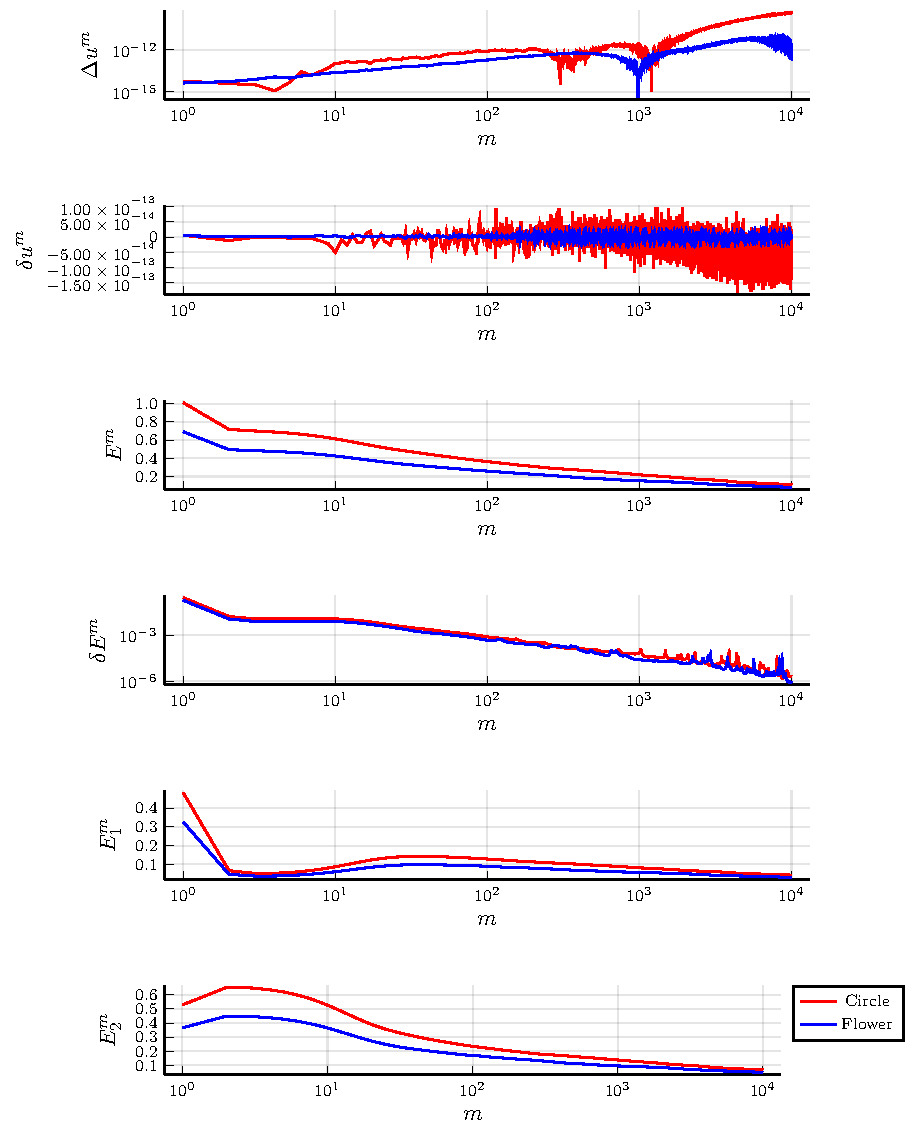
\includegraphics{results/physical_CH_plot.pdf}
    \caption{Evolution of the  global mass conservation $\Delta u^m$, and the local mass difference $\delta u^m$ total discrete energies $E^m$,$E^m_{1}$,$E^m_{2}$, with the corresponding local energy difference $\delta E^m$, on a circular domain and a flower-shaped domain. }
    \label{fig:physical_CH_plot}
\end{figure}


\begin{figure}[]
    \centering
    \hfill
    \subfloat[$m=0$]{
        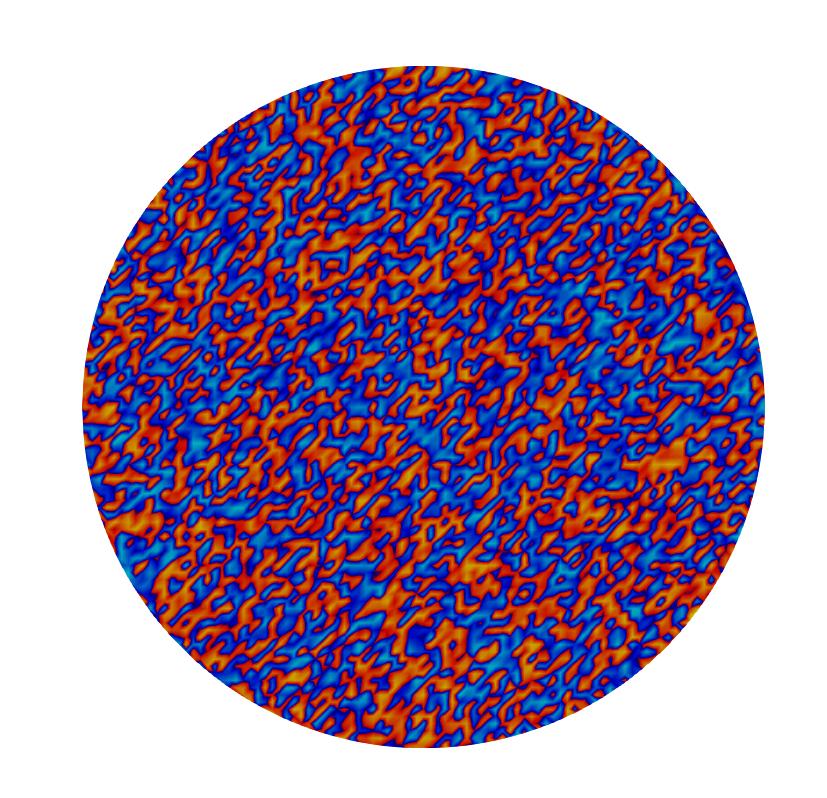
\includegraphics[width=0.3\textwidth]{results/illustration/c0.png}
    }\hfill
    \subfloat[$m=2$]{
        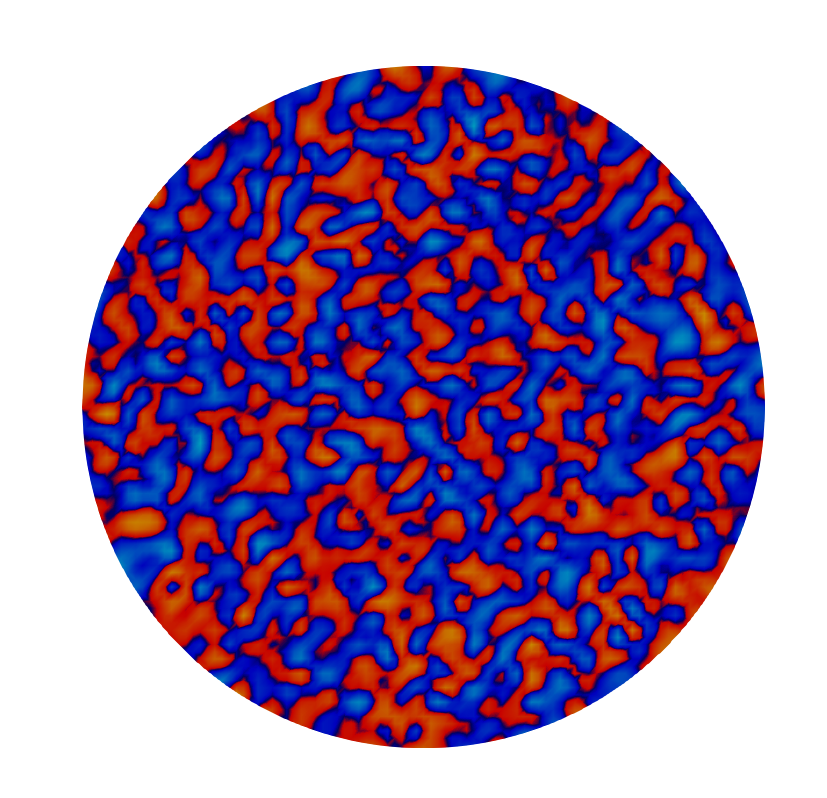
\includegraphics[width=0.3\textwidth]{results/illustration/c2.png}
    }
    \hfill
    \subfloat[$m=10$]{
        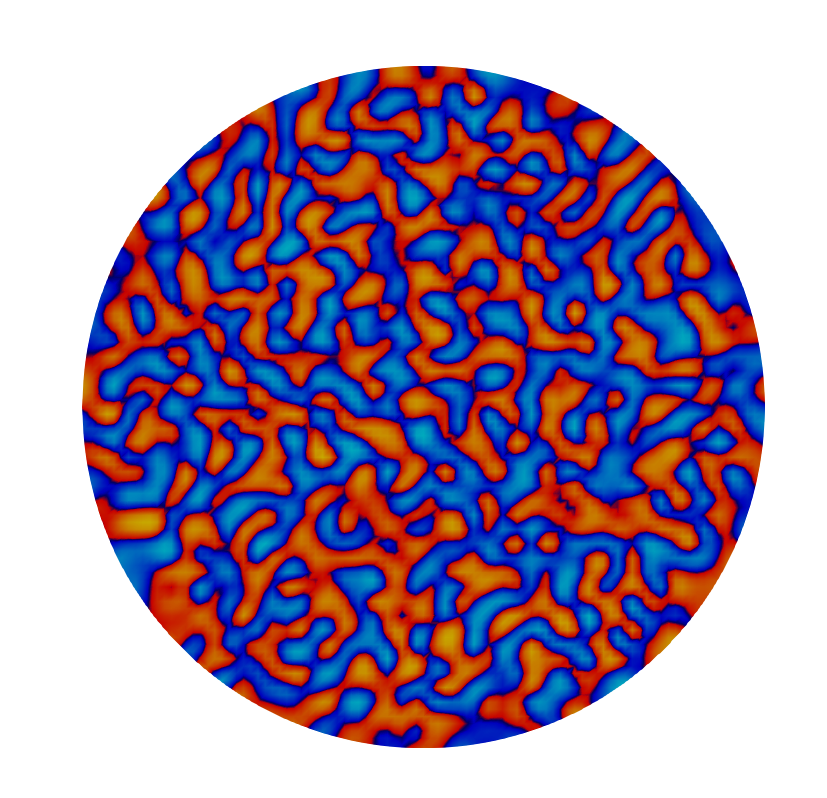
\includegraphics[width=0.3\textwidth]{results/illustration/c10.png}
    }
    \\
    \vspace{10pt}
    \hfill
    \subfloat[$m=50$]{
        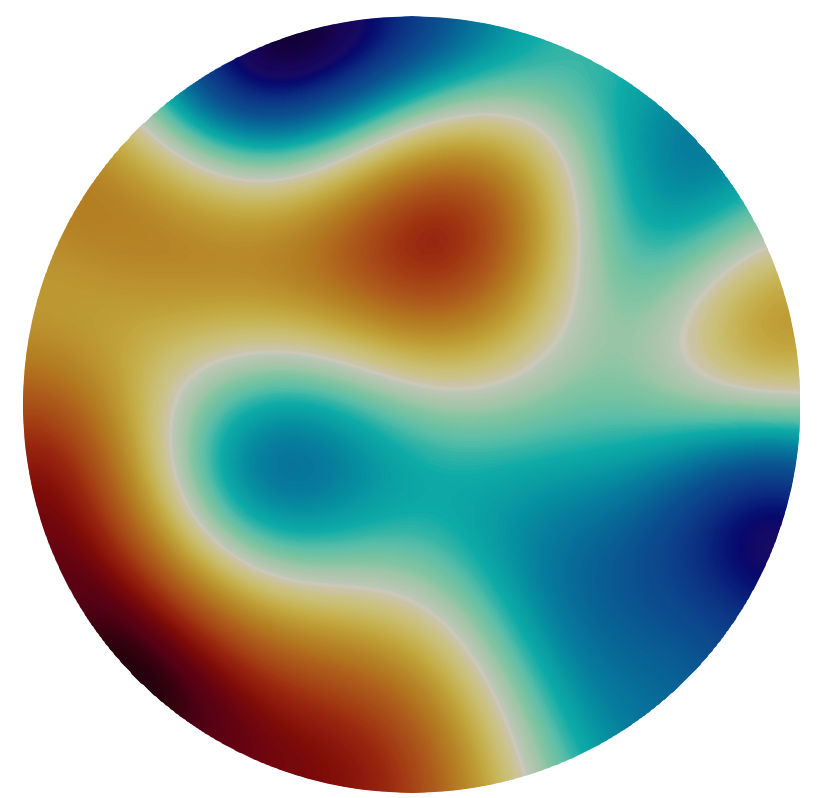
\includegraphics[width=0.3\textwidth]{results/illustration/c50.png}
    }
    \hfill
    \subfloat[$m=200$]{
        
\includegraphics[width=0.3\textwidth]{results/illustration/c200.png}
    }\hfill
    \subfloat[$m=500$]{
        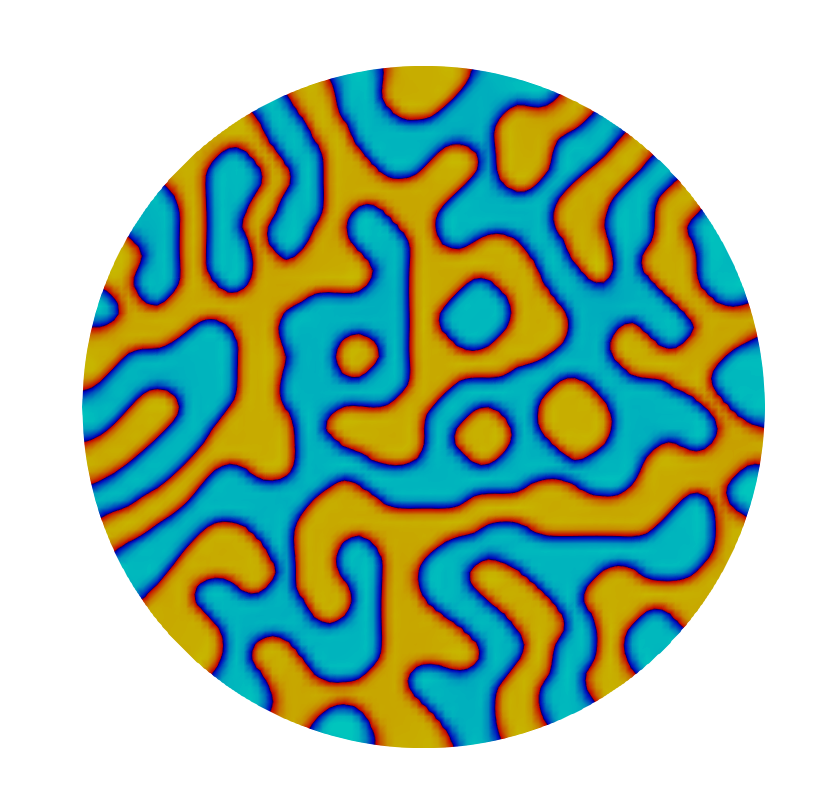
\includegraphics[width=0.3\textwidth]{results/illustration/c500.png}
    }
    \\
    \vspace{10pt}
    \hfill
    \subfloat[$m=1000$]{
        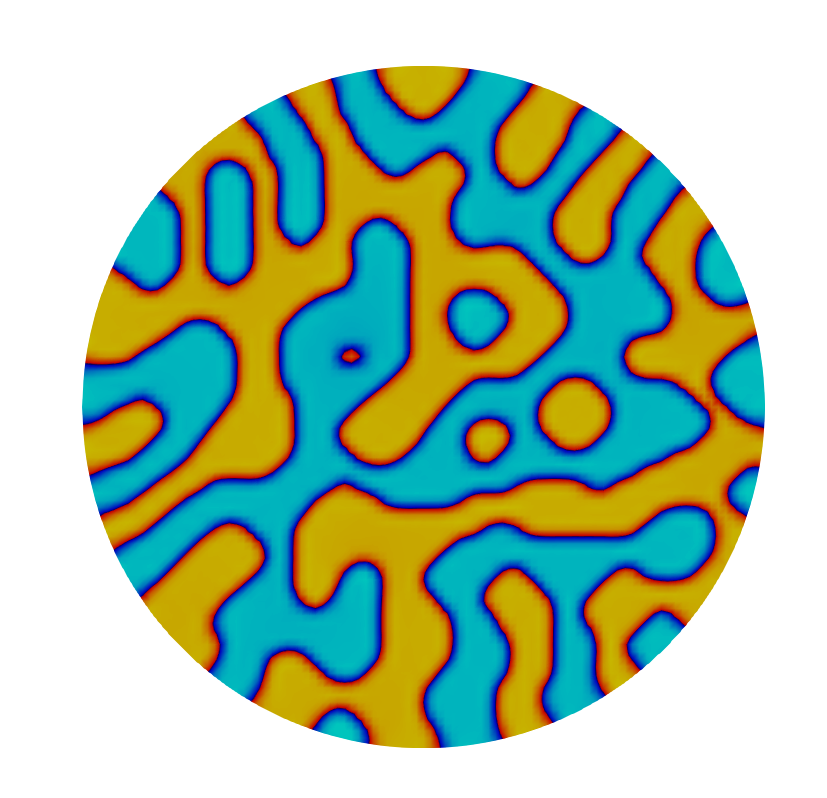
\includegraphics[width=0.3\textwidth]{results/illustration/c1000.png}
    }
    \hfill
    \subfloat[$m=5000$]{
        
\includegraphics[width=0.3\textwidth]{results/illustration/c5000.png}
    }\hfill
    \subfloat[$m=10000$]{
        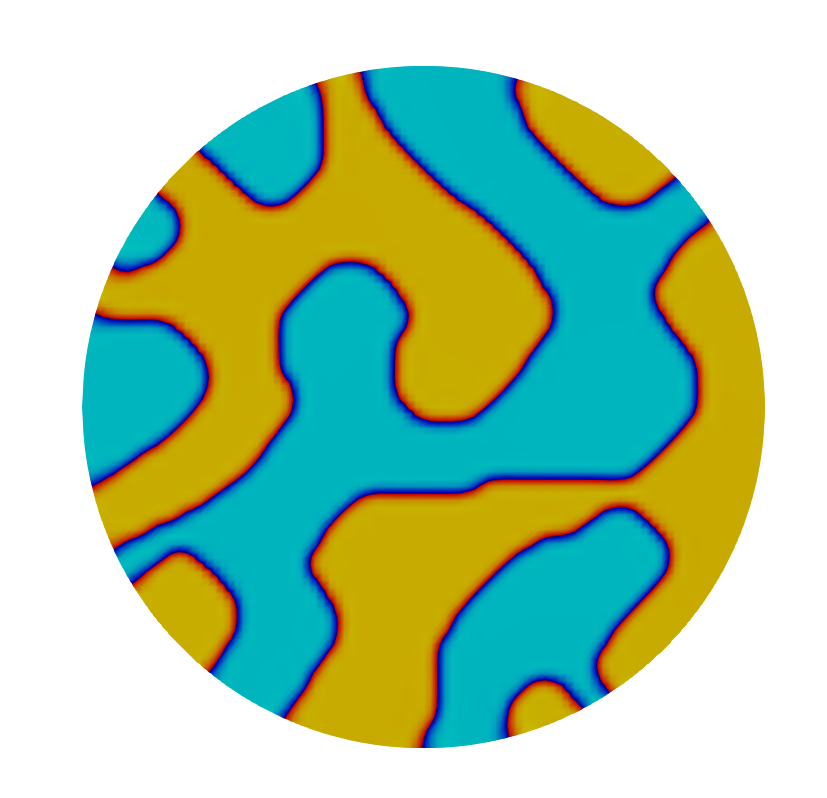
\includegraphics[width=0.3\textwidth]{results/illustration/c10000.png}
    }
    \vspace{10pt}
        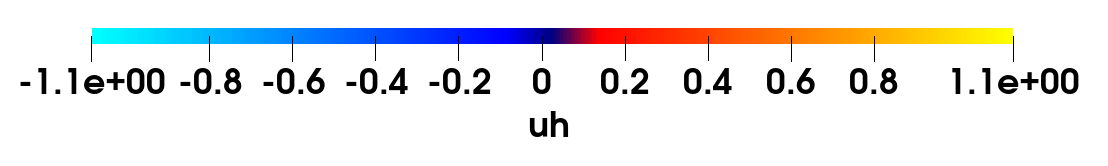
\includegraphics[width=0.8\textwidth]{results/illustration/colobar.png}

    \caption{Illustration of simulations of the Cahn-Hilliard equation on the circle domain for $t\in \left[ 0, 10000\tau  \right] $.}
        \label{sub:fig:ill_circle}
\end{figure}

\begin{figure}[]
    \centering
    \hfill
    \subfloat[$m=0$]{
        
\includegraphics[width=0.3\textwidth]{results/illustration/f0.png}
    }\hfill
    \subfloat[$m=2$]{
        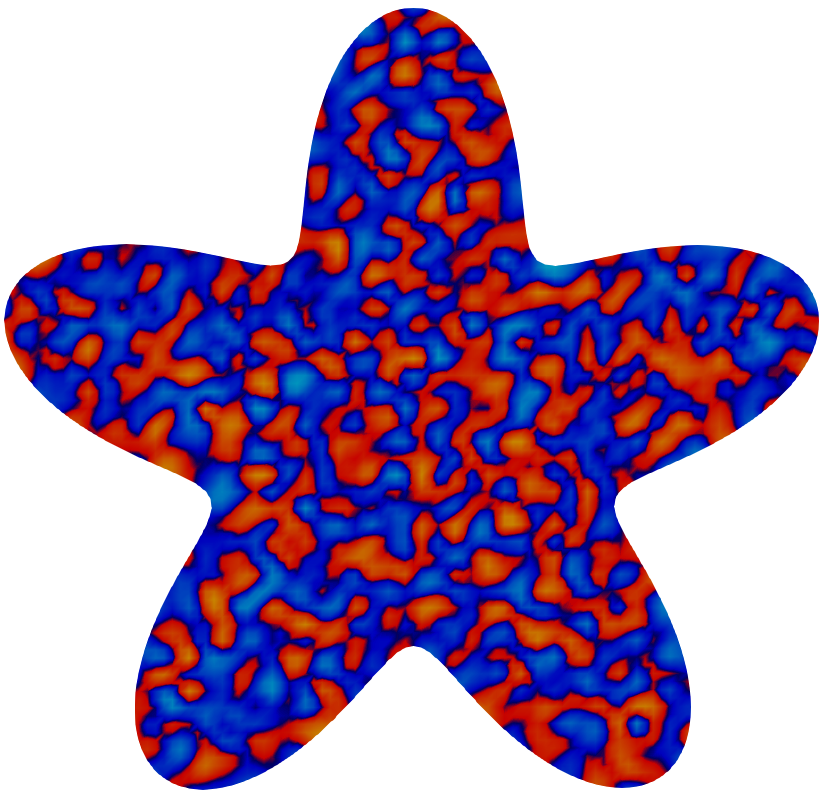
\includegraphics[width=0.3\textwidth]{results/illustration/f2.png}
    }
    \hfill
    \subfloat[$m=10$]{
        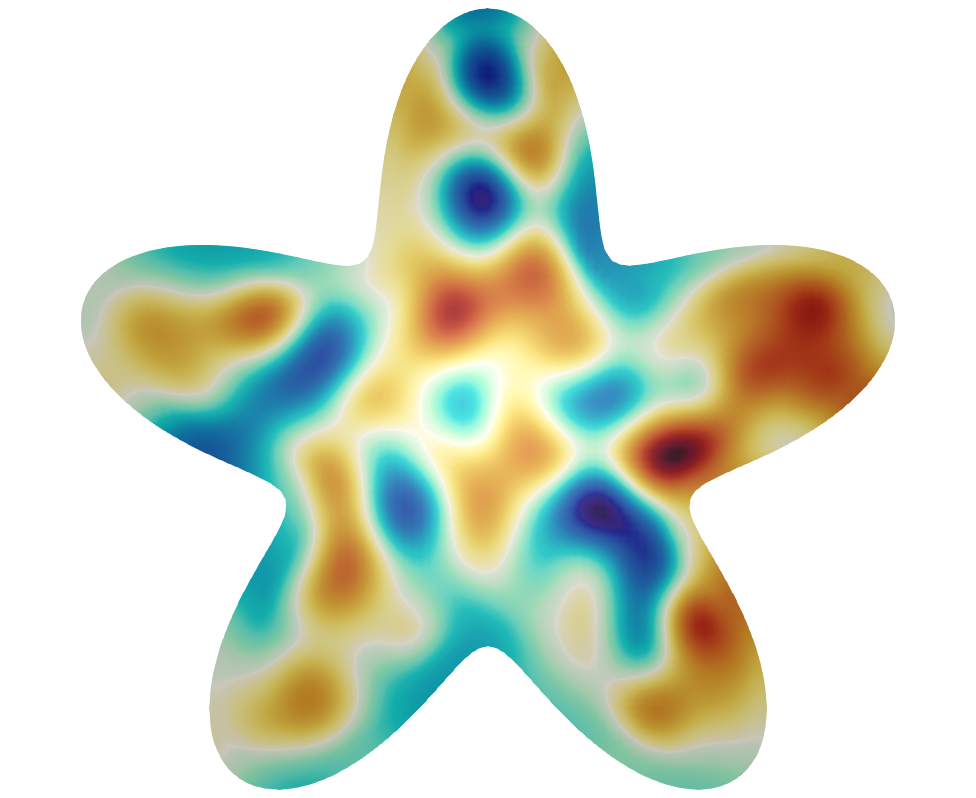
\includegraphics[width=0.3\textwidth]{results/illustration/f10.png}
    }
    \\
    \vspace{10pt}
    \hfill
    \subfloat[$m=50$]{
        
\includegraphics[width=0.3\textwidth]{results/illustration/f50.png}
    }
    \hfill
    \subfloat[$m=200$]{
        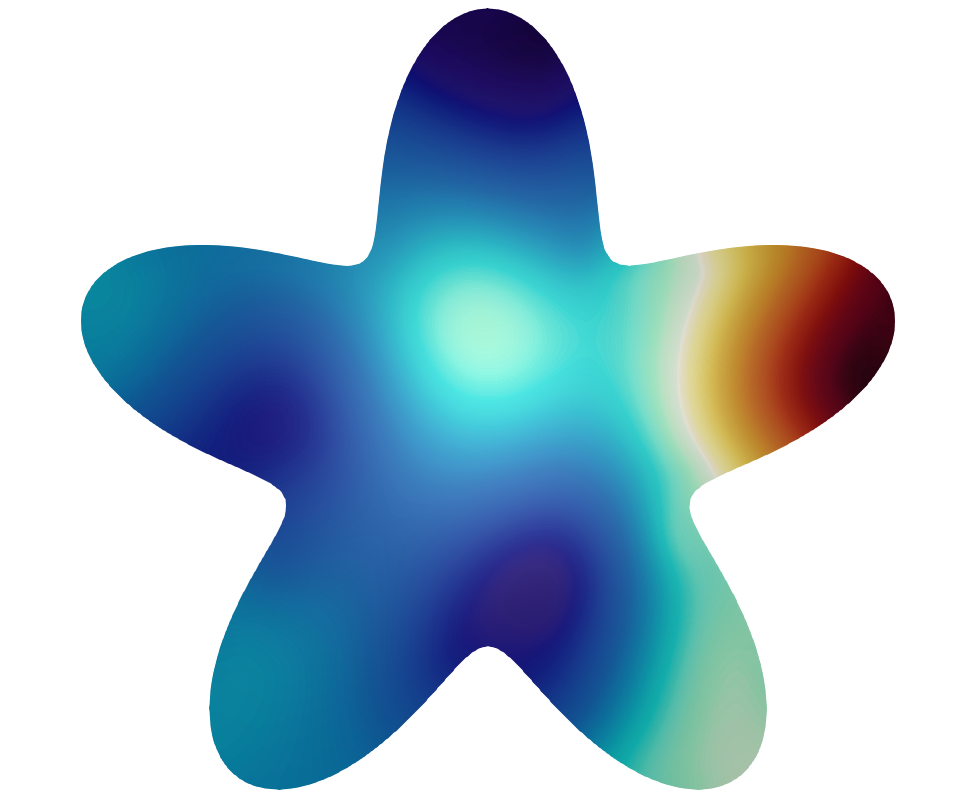
\includegraphics[width=0.3\textwidth]{results/illustration/f200.png}
    }\hfill
    \subfloat[$m=500$]{
        
\includegraphics[width=0.3\textwidth]{results/illustration/f500.png}
    }
    \\
    \vspace{10pt}
    \hfill
    \subfloat[$m=1000$]{
        
\includegraphics[width=0.3\textwidth]{results/illustration/f1000.png}
    }
    \hfill
    \subfloat[$m=5000$]{
        
\includegraphics[width=0.3\textwidth]{results/illustration/f5000.png}
    }\hfill
    \subfloat[$m=10000$]{
        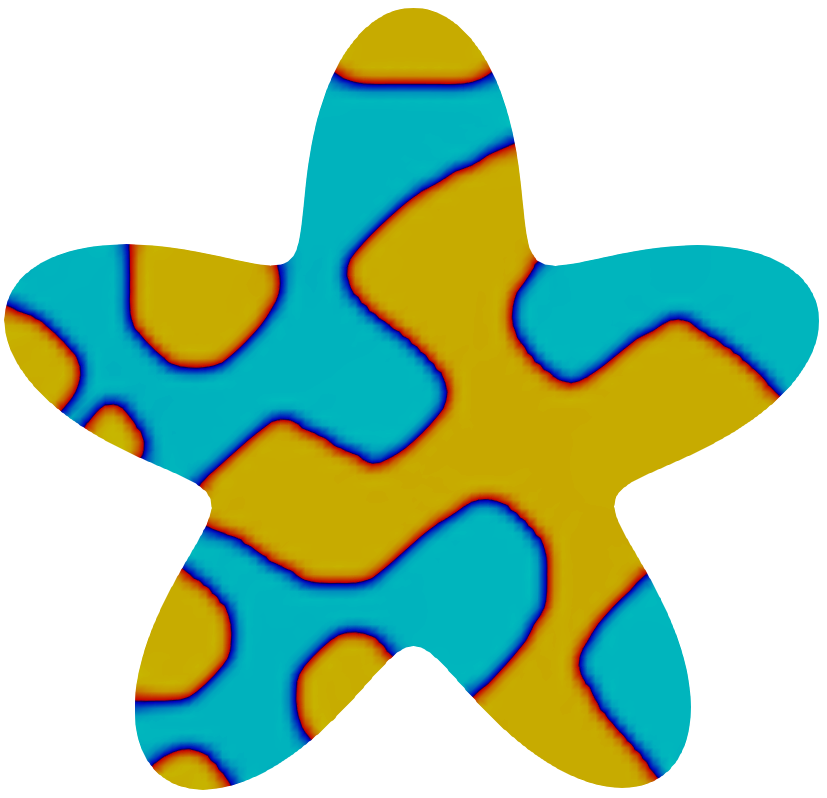
\includegraphics[width=0.3\textwidth]{results/illustration/f10000.png}
    }
    \vspace{10pt}
        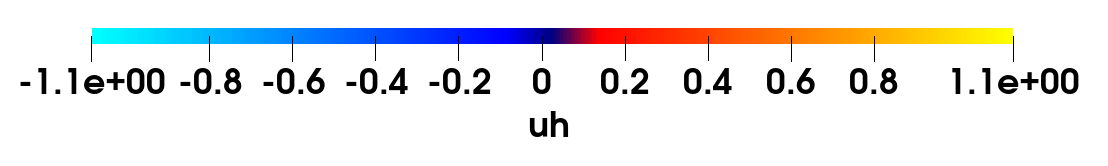
\includegraphics[width=0.8\textwidth]{results/illustration/colobar.png}
    \caption{Illustration of simulations of the Cahn-Hilliard equation on the flower domain for $t\in \left[ 0, 10000\tau  \right] $.}
        \label{sub:fig:ill_flower}
\end{figure}



In our experiments, we defined the initial function $u_{0}(x)$ as the uniform samples from the interval $[-1, 1]$ for each node. That is, for each node $a_{i}$, $u_{0}(a_{i})$ is a sample from the uniform distribution on the interval $[-1, 1]$. This
applies for all $i = 1, \ldots, N$, where $N$ is the total number of degrees of freedom in our system. The node $a_{i}$ is associated with the nodal basis for all $N$ degrees of freedom, as discussed for the discrete system
\eqref{eq:discretized_system}. We again used a square background mesh with length $L=2.7$ and mesh size $h=\frac{L}{n}$ for $n=2^{7}$. For an illustration of the active set $\mathcal{T}_{h} $ (defined in Section \ref{sub:unfitted_mesh}), see Figure \ref{sub:fig:active_mesh}.

\begin{figure}[H]
    \centering
    \hfill
    % \subfloat[]{
        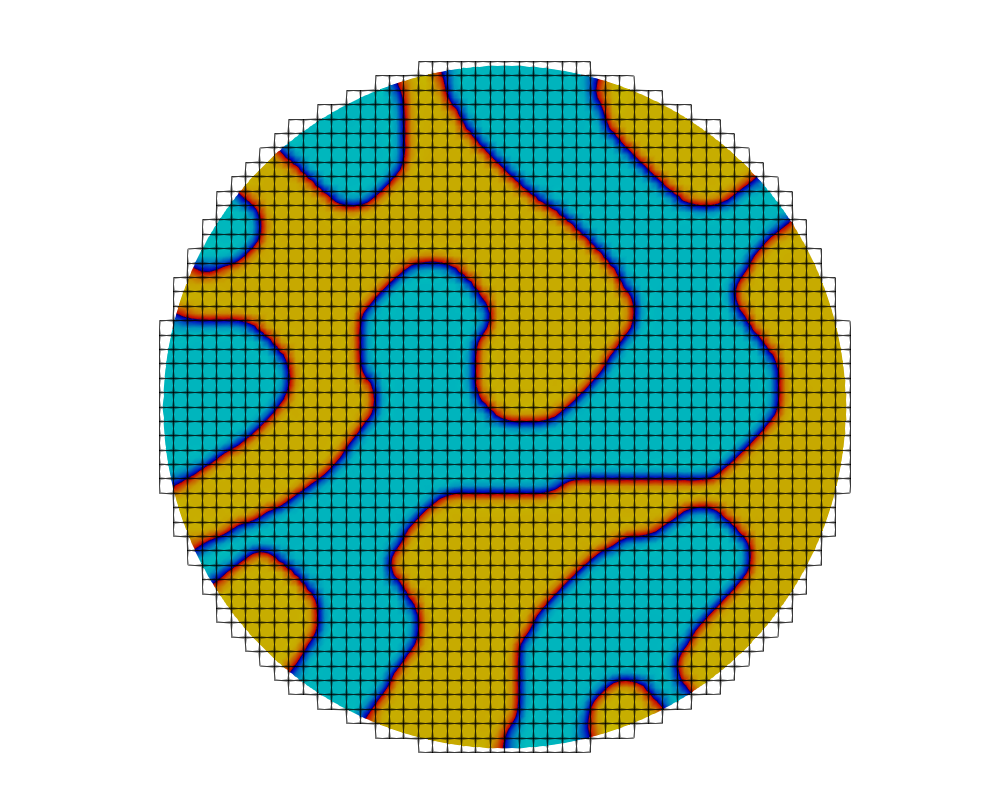
\includegraphics[width=0.45\textwidth]{results/illustration/active_circle.png}
    % }
    \hfill
    % \subfloat[]{
        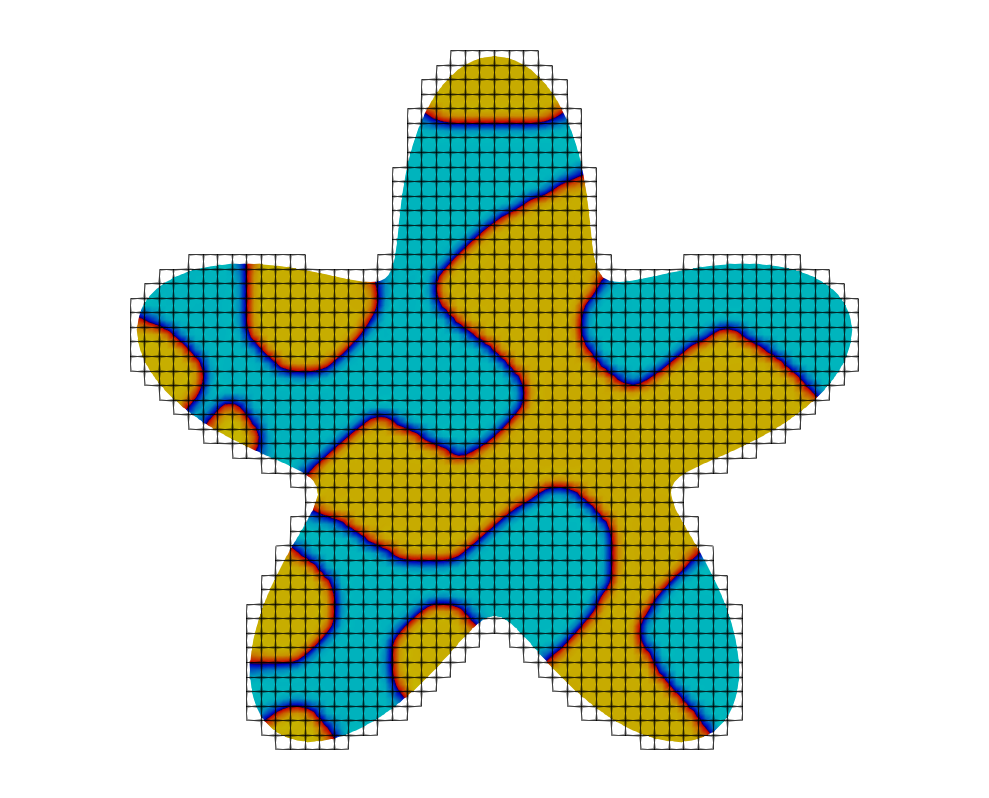
\includegraphics[width=0.45\textwidth]{results/illustration/active_flower.png}
    % }
    \caption{Illustration of the active mesh $\mathcal{T}_{h} $.}
    \label{sub:fig:active_mesh}
\end{figure}


We ran the simulation on the for the flower domain \eqref{eq:flower} and the circular domain \eqref{eq:circle}, illustrated in Figure \ref{sub:fig:ill_flower} and \ref{sub:fig:ill_circle}. The corresponding plots of the mass conservation and energy decrease are presented
in the Figure \ref{fig:physical_CH_plot}, and confirm the expected physical properties of the Cahn-Hilliard equation. The global relative error $\Delta u^{m}_{h}$ and $\delta u^{m}_{h}$ demonstrating that the mass is conserved. We also observe that the energy functional
$E(u_h)$ monotonically decreases over time and that $\delta E^{m} >0$, signifying the systems tendency to seek a state of minimal energy. Take note that $E^{m}{1}$ and $E^{m}{2}$ are interconnected in such a way that if the value of one increases, the other will correspondingly decrease to maintain balance, and vice versa.



\subsection{Note on the manufactured solution}%
\label{sub:the_problem}

While the report is not consisting of a numerical convergence analysis of the Cahn-Hilliard problem, we still present a framework for manufactured solutions for non-homogeneous boundary conditions. Let $ u( x,0) =  u_{0}$ then is Cahn-Hilliard with
non-homogeneous boundary conditions as follows,
\begin{subequations}
    \label{eq:ch_gen}
    \begin{align}
    \label{eq:ch_gen:a}
        \partial _{t} u + \Delta  \left(  \varepsilon^2  \Delta u - f( u) \right)   &= g_{0}( x)   \quad \text{ in } \Omega,  \\
        \partial _{n} u &= g_{1}( x)  \quad \text{ on } \Gamma,  \\
        \partial _{n}    \Delta u   &= g_{2}(x)  \quad \text{ on } \Gamma,
    \end{align}
\end{subequations}
where we defined $f( u) = F'( u) =u( u^2 -1)  $ for $F( u) = \frac{1}{4}( u^{2} - 1)^{2} $ and the domain $\Omega \subset \mathbb{R} ^{d} $  for $d = 2,3$. In contrast to the standard version presented in the introduction \eqref{eq:strongch}, this
version is generalized to also holds for for functions $g_{0},g_{1},g_{2}: \Omega \to\mathbb{R}   $. While the standard version may be physical correct, this version creates flexibility so we can easily construct manufactured solution on complex domains.

    Designing a manufactured solution using $g_{0}( \cdot ) $ may be temping with the formulation \eqref{eq:ch_gen:a}. However, observe that expanding the Laplacian we get,
    \begin{equation}
    \begin{split}
        \Delta  \left(  \varepsilon^2  \Delta u - f( u) \right) & = \varepsilon^2 \Delta^2 u -  \Delta f( u) \\
                                                                                    &= \varepsilon^{2} \Delta ^2 u  - 3( 2u \| \nabla u \|_{ 2 }^{ 2 } + u^{2}  \Delta u )   \\
    \end{split}
    \end{equation}
Here we applied the chain rule twice and inserted the derivatives.
\begin{equation}
    \label{eq:nonlinear_laplace}
    \begin{split}
\Delta f( u)  &= \nabla \cdot \nabla f( u)  = \nabla \cdot  \left[ f' ( u) \partial _{x_{1}}u, \ldots, f' ( u) \partial _{x_{d}}u \right] ^{T} \\
& =  f'' ( u)( ( \partial _{x_{1}}u )^{2} + \ldots +( \partial _{x_{d}}u )^{2} ) +  f' ( u)( \partial _{x_{1} x_{1}}u + \ldots +   \partial _{x_{d} x_{d}}u ) \\
&=  f'' ( u) \| \nabla u \|_{ 2 }^{ 2 } + f' ( u)  \Delta u  = 6u \| \nabla u \|_{ 2 }^{ 2 } + 3u^{2}  \Delta u
    \end{split}
\end{equation}

% Our goal is to write the Cahn Hilliard equation on weak form.
% Assume that $\Omega  \subset \mathbb{R} ^{d}$ with a $\Gamma $ in $C^2$.
%  Let $u \in  H^{4}( \Omega ) $ and $v \in V_{h} $.
% Now, expanding the first Laplace operator from a weak point of view is it clear that
% \[
%  ( \Delta ( \varepsilon  \Delta u - \frac{1}{\varepsilon } f( u) ) ,v )_{\Omega } = \varepsilon ( \Delta^{2} u ,v )_{\Omega } - \frac{1}{\varepsilon } ( \Delta f( u)  ,v )_{\Omega }.
% \]
% Hence, this makes it natural to associate the biharmonic $( \Delta ^2 u,v)_{\Omega } $ with bilinear forms $A_{h}( \cdot ,\cdot ) $ , however, in this section will we only consider the Laplace
% variant $a^{L}( \cdot ,\cdot ) $.
We now seek to find a weak form of the nonlinear term with non homogeneous boundary conditions.
\begin{lemma}[Semi-linear form]
    Let $u \in H^4( \Omega ) $ be solution to \eqref{eq:ch_gen} and $v_{h} \in V_{h}$ the test function.
Then can we rewrite the nonlinear term into the corresponding semi-linear form $c_{h}( \cdot ,\cdot )  $ for the nonlinear term $( -\Delta f( u) , v_{h})_{\Omega }$ into two consistent formulations.
\begin{align}
    \label{eq:ch:1}
      c^{1}_{h} ( u,v_{h})  & = ( f' ( u) \nabla u, \nabla v_{h} )_{\Omega }  - ( f'( u)  g_{1}   ,  v_{h})_{\Gamma } \\
    \label{eq:ch:2}
        c^{2}_{h} ( u,v_{h})  & = -( f( u), \Delta v_{h} )_{\Omega }+  ( f( u) , \jump{ \partial _{n}v_{h} }  )_{\mathcal{F} _{h}^{int}} + ( f(u), \partial _{n} v_{h})_{\Gamma  }  - ( f'( u)  g_{1}   ,  v_{h})_{\Gamma }
\end{align}
% \begin{remark}
%     Be aware that the both formulations are consistent and if we replace $u \in H^{4}( \Omega ) $ with  $u_{h} \in  V_{h}$ we have two different discrete formulations.
% \end{remark}

\end{lemma}
% \todo[inline]{ I criticize \cite[ Remark 4.1d]{feng2007fully} which says that says that finding this weak form is not possible for conforming methods (I guess $C^{0}$ is a conforming method??). }

\begin{proof}

         \textbf{Derivation of \eqref{eq:ch:1}.  }  We want to construct the first formulation. Let $T$ be an element in $\mathcal{T}_{h}$. From Greens theorem is it easy to see that
            \begin{equation}
            \label{eq:1_gr}
-(\Delta f( u) , v_{h})_{T } = (\nabla f( u), \nabla v_{h}  )_{T } - ( \partial _{n}  f( u), v_{h} )_{\partial T }
            \end{equation}
            First by utilizing that $\nabla f( u) = f' ( u) \nabla u $ and $\partial _{n}f( u)  = f' ( u)  \partial _{n}u$  and doing a summation over the triangles  is it clear that \[
            ( -\Delta f( u),v_{h} )_{\Omega  } =(f' ( u) \nabla u, \nabla v_{h}  )_{\Omega  } - (   f' ( u)\partial _{n}u, v_{h} )_{\partial \mathcal{T}_{h}  }
            \]
            Iterating over the facets is it clear that \[
                \begin{split}
            (   f' ( u)\partial _{n}u, v_{h} )_{\partial \mathcal{T}_{h}  } & = \sum_{F \in \mathcal{F}_{h}  }^{} \int_{F}^{}   \jump{ f' ( u)\partial _{n}u, v_{h} } \\
                                                                        & =  ( \jump{ f' ( u) \partial _{n}u },  \mean{v_{h}}    )_{\mathcal{F}^{int}_{h} } + ( \mean{ f' ( u) \partial _{n}u }, \jump{ v_{h} }    )_{\mathcal{F}^{int}_{h} } +  ( f' ( u)
                                                                        \partial _{n}u, v_{h}) _{\Gamma } \\
                                                                        & =  ( f' ( u) \partial _{n}u, v_{h}) _{\Gamma }
                \end{split}
            \]
            The jump terms vanishes by the regularity of $u$ and $v_{h}$. Hence, by inserting $g_{1}$ we have shown that the first formulation holds.

         \textbf{Derivation of \eqref{eq:ch:2}.  }  Applying a extra iteration of Greens theorem on \eqref{eq:1_gr} we get the following terms.
\[
    \begin{split}
-(\Delta f( u) , v_{h})_{T }  = -( f( u), \Delta v_{h} )_{T} + (f( u), \partial _{n} v_{h}  )_{\partial T} - (   f'( u)\partial _{n}u, v_{h} )_{\partial T } .
    \end{split}
\]
Now, by doing a summation of all triangles it is clear that this holds.
\begin{equation}
\label{eq:f_g2}
-(\Delta f( u) , v_{h})_{\Omega  }  = -( f( u), \Delta v_{h} )_{\Omega } + (f( u), \partial _{n} v_{h}  )_{\partial \mathcal{T}_{h} } - (   f'( u)\partial _{n}u, v_{h} )_{\partial \mathcal{T}_{h}  }
\end{equation}
It comes evident from the first step of the proof that $ (   f'( u)\partial _{n}u, v_{h} )_{\partial \mathcal{T}_{h}  } = (   f'( u)\partial _{n}u, v_{h} )_{\Gamma }$, hence, we only need to compute the term $(f( u), \partial _{n} v_{h}  )_{\partial
\mathcal{T}_{h} }$ on the facets. \[
    \begin{split}
(f( u), \partial _{n} v_{h}  )_{\partial
\mathcal{T}_{h} } & = \sum_{F\in \mathcal{F} _{h}}^{} \int_{F}^{}\jump{ f( u), \partial _{n} v_{h}  } \\
& =  (\jump{ f( u)  }  , \mean{ \partial _{n} v_{h} }    )_{ \mathcal{F}_{h}^{int} } +(\mean{ f( u)  }  , \jump{ \partial _{n} v_{h} }    )_{ \mathcal{F}_{h}^{int} } + (f( u), \partial _{n} v_{h}  )_{\Gamma } \\
&=  (\mean{ f( u)  }  , \jump{ \partial _{n} v_{h} }    )_{ \mathcal{F}_{h}^{int} } + (f( u), \partial _{n} v_{h}  )_{\Gamma }
    \end{split}
\]
Again one of the jump terms vanishes because of the regularity of $u$.
Inserting the result into \eqref{eq:f_g2} have we shown that the second formulation also holds.
\end{proof}


Combining the full general Cahn-Hilliard problem in \eqref{eq:ch_gen} with the semi-linear forms\eqref{eq:ch:1} and the CutCIP biharmonic problem \eqref{eq:discrete_CutCIP_prob}, we get the following scheme.
\begin{equation}
    ( \partial _{t}u_{h}, v_{h})_\Omega + \varepsilon^2  A_{h}( u_{h},v_{h}) + c_{h}( u_{h},v_{h})   =   l_{h}(v_{h}) \quad  \forall u_{h}, v_{h} \in V_{h}
\end{equation}

To illustrate, assume we use the Laplace formulation presented in \eqref{eq:laplace_prob} integrated into \eqref{eq:discrete_CutCIP_prob}, i.e. $A_{h}( u_{h}, v_{h}) = a^{L}_{h}( u_{h}, v_{h}) + g_{h}( u_{h}, v_{h})   = l_{h}^{L}( v_{h})$. Due to the $\varepsilon $ scaling, we ultimately
arrive at the following modification.
 \begin{equation}
    l_{h}^{L}( v_{h})  =  \left( g_{0}, v_{h} \right) _{\Omega } -  \varepsilon^2 ( g_{2},  v_{h} )_{\Gamma }  -  \varepsilon^2 ( g_{1}, \Delta  v_{h}  )_{\Gamma }  + \varepsilon^2 \frac{\gamma }{h} ( g_{1}, \partial _{n} v_{h}  )_{\Gamma }
 \end{equation}
 Hence, we arrived at a system which can easily be used to construct manufactured solution.


    % 
\newpage
\section{Numerical results}%
\label{sec:numerical_results}


\begin{table}[h!]
    \caption{Convergence analysis of the numerical method}
    \label{table:CutFEM_error1}
  \begin{tabular}{rrrrrrrrr}
    \hline\hline
    \textbf{$n$} & \textbf{$\Vert e \Vert_{L^2}$} & \textbf{EOC} & \textbf{$ \Vert e \Vert_{H^1}$} & \textbf{EOC} & \textbf{$\Vert e \Vert_{ a_h,* }$} & \textbf{EOC} & \textbf{Cond number} & \textbf{ndofs} \\\hline
    8 & 1.6E+01 &  & 1.3E+02 &  & 3.6E+03 &  & 3.0E+05 & 2.4E+02 \\
    16 & 3.7E+00 & 2.14 & 3.1E+01 & 2.09 & 1.0E+03 & 1.78 & 2.2E+06 & 8.3E+02 \\
    32 & 8.3E-01 & 2.15 & 7.4E+00 & 2.09 & 2.9E+02 & 1.83 & 1.6E+07 & 3.0E+03 \\
    64 & 2.3E-01 & 1.87 & 1.8E+00 & 2.03 & 8.0E+01 & 1.86 & 1.3E+08 & 1.1E+04 \\
    128 & 5.0E-02 & 2.19 & 4.4E-01 & 2.04 & 2.6E+01 & 1.63 & 1.0E+09 & 4.3E+04 \\
    256 & 1.3E-02 & 1.92 & 1.1E-01 & 2.01 & 8.4E+00 & 1.63 & 7.9E+09 & 1.7E+05 \\\hline\hline
  \end{tabular}

\end{table}

\begin{figure}[h!]
    \centering
    \begin{table}
  \begin{tabular}{rrrrrrrrr}
    \noalign{\hrule height 2pt}
    \textbf{$n$} & \textbf{$\Vert e \Vert_{L^2}$} & \textbf{EOC} & \textbf{$ \Vert e \Vert_{H^1}$} & \textbf{EOC} & \textbf{$\Vert e \Vert_{ a_h,* }$} & \textbf{EOC} & \textbf{Cond number} & \textbf{ndofs} \\\noalign{\hrule height 2pt}
    8 & 1.4E-01 & NaN & 7.3E-01 & NaN & 7.4E+00 & NaN & 1.7E+05 & 1.8E+02 \\
    16 & 3.4E-02 & 2.03 & 2.0E-01 & 1.87 & 3.8E+00 & 0.97 & 9.2E+05 & 4.8E+02 \\
    32 & 1.0E-02 & 1.74 & 4.9E-02 & 2.02 & 1.8E+00 & 1.06 & 6.6E+06 & 1.6E+03 \\
    64 & 2.7E-03 & 1.88 & 1.2E-02 & 2.03 & 9.0E-01 & 1.03 & 5.0E+07 & 5.6E+03 \\
    128 & 7.0E-04 & 1.97 & 3.1E-03 & 1.99 & 4.4E-01 & 1.01 & 3.9E+08 & 2.1E+04 \\
    256 & 2.2E-04 & 1.64 & 8.2E-04 & 1.90 & 2.2E-01 & 1.01 & 3.0E+09 & 8.1E+04 \\\noalign{\hrule height 2pt}
  \end{tabular}
\end{table}

    \caption{The plot presents the error in $L^2$, $H^1$ the energy norm ($\Vert e \Vert_{a_h,*}$) with order 2 of the CutCIP method (Laplace).}
    \label{fig:CutFEM_error1}
\end{figure}

\begin{figure}[h!]
    \centering
    \begin{subfigure}{0.49\textwidth}
        \centering
        
% Recommended preamble:
% \usetikzlibrary{arrows.meta}
% \usetikzlibrary{backgrounds}
% \usepgfplotslibrary{patchplots}
% \usepgfplotslibrary{fillbetween}
% \pgfplotsset{%
%     layers/standard/.define layer set={%
%         background,axis background,axis grid,axis ticks,axis lines,axis tick labels,pre main,main,axis descriptions,axis foreground%
%     }{
%         grid style={/pgfplots/on layer=axis grid},%
%         tick style={/pgfplots/on layer=axis ticks},%
%         axis line style={/pgfplots/on layer=axis lines},%
%         label style={/pgfplots/on layer=axis descriptions},%
%         legend style={/pgfplots/on layer=axis descriptions},%
%         title style={/pgfplots/on layer=axis descriptions},%
%         colorbar style={/pgfplots/on layer=axis descriptions},%
%         ticklabel style={/pgfplots/on layer=axis tick labels},%
%         axis background@ style={/pgfplots/on layer=axis background},%
%         3d box foreground style={/pgfplots/on layer=axis foreground},%
%     },
% }

\begin{tikzpicture}[/tikz/background rectangle/.style={fill={rgb,1:red,1.0;green,1.0;blue,1.0}, fill opacity={1.0}, draw opacity={1.0}}, show background rectangle]
\begin{axis}[point meta max={nan}, point meta min={nan}, legend cell align={left}, legend columns={1}, title={}, title style={at={{(0.5,1)}}, anchor={south}, font={{\fontsize{14 pt}{18.2 pt}\selectfont}}, color={rgb,1:red,0.0;green,0.0;blue,0.0}, draw opacity={1.0}, rotate={0.0}, align={center}}, legend style={color={rgb,1:red,0.0;green,0.0;blue,0.0}, draw opacity={1.0}, line width={1}, solid, fill={rgb,1:red,1.0;green,1.0;blue,1.0}, fill opacity={1.0}, text opacity={1.0}, font={{\fontsize{8 pt}{10.4 pt}\selectfont}}, text={rgb,1:red,0.0;green,0.0;blue,0.0}, cells={anchor={center}}, at={(1.02, 1)}, anchor={north west}}, axis background/.style={fill={rgb,1:red,1.0;green,1.0;blue,1.0}, opacity={1.0}}, anchor={north west}, xshift={1.0mm}, yshift={-1.0mm}, width={145.4mm}, height={99.6mm}, scaled x ticks={false}, xlabel={$\delta$}, x tick style={color={rgb,1:red,0.0;green,0.0;blue,0.0}, opacity={1.0}}, x tick label style={color={rgb,1:red,0.0;green,0.0;blue,0.0}, opacity={1.0}, rotate={0}}, xlabel style={at={(ticklabel cs:0.5)}, anchor=near ticklabel, at={{(ticklabel cs:0.5)}}, anchor={near ticklabel}, font={{\fontsize{11 pt}{14.3 pt}\selectfont}}, color={rgb,1:red,0.0;green,0.0;blue,0.0}, draw opacity={1.0}, rotate={0.0}}, xmajorgrids={true}, xmin={-0.001471665988344504}, xmax={0.05052719893316125}, xticklabels={{$0.00$,$0.01$,$0.02$,$0.03$,$0.04$,$0.05$}}, xtick={{0.0,0.010000000000000002,0.020000000000000004,0.030000000000000006,0.04000000000000001,0.05000000000000001}}, xtick align={inside}, xticklabel style={font={{\fontsize{8 pt}{10.4 pt}\selectfont}}, color={rgb,1:red,0.0;green,0.0;blue,0.0}, draw opacity={1.0}, rotate={0.0}}, x grid style={color={rgb,1:red,0.0;green,0.0;blue,0.0}, draw opacity={0.1}, line width={0.5}, solid}, axis x line*={left}, x axis line style={color={rgb,1:red,0.0;green,0.0;blue,0.0}, draw opacity={1.0}, line width={1}, solid}, scaled y ticks={false}, ylabel={$\kappa(A)$}, y tick style={color={rgb,1:red,0.0;green,0.0;blue,0.0}, opacity={1.0}}, y tick label style={color={rgb,1:red,0.0;green,0.0;blue,0.0}, opacity={1.0}, rotate={0}}, ylabel style={at={(ticklabel cs:0.5)}, anchor=near ticklabel, at={{(ticklabel cs:0.5)}}, anchor={near ticklabel}, font={{\fontsize{11 pt}{14.3 pt}\selectfont}}, color={rgb,1:red,0.0;green,0.0;blue,0.0}, draw opacity={1.0}, rotate={0.0}}, ymode={log}, log basis y={10}, ymajorgrids={true}, ymin={100000.0}, ymax={1.0e25}, yticklabels={{$10^{5}$,$10^{10}$,$10^{15}$,$10^{20}$,$10^{25}$}}, ytick={{100000.0,1.0e10,1.0e15,1.0e20,1.0e25}}, ytick align={inside}, yticklabel style={font={{\fontsize{8 pt}{10.4 pt}\selectfont}}, color={rgb,1:red,0.0;green,0.0;blue,0.0}, draw opacity={1.0}, rotate={0.0}}, y grid style={color={rgb,1:red,0.0;green,0.0;blue,0.0}, draw opacity={0.1}, line width={0.5}, solid}, axis y line*={left}, y axis line style={color={rgb,1:red,0.0;green,0.0;blue,0.0}, draw opacity={1.0}, line width={1}, solid}, colorbar={false}]
    [\addlegendimage{empty legend}] \addlegendentry[font={{\fontsize{11 pt}{14.3 pt}\selectfont}}, text={rgb,1:red,0.0;green,0.0;blue,0.0}] {\hspace{-.6cm}{\textbf{$(\gamma, \gamma_1, \gamma_2)$}}}
    \addplot[color={rgb,1:red,0.0;green,0.0;blue,1.0}, name path={d224c932-a57b-4b2d-b00b-6e21c1ac3de3}, draw opacity={1.0}, line width={1}, solid]
        table[row sep={\\}]
        {
            \\
            0.0  1.2679162841962957e8  \\
            0.012263883236204186  1.2718633259851372e8  \\
            0.024527766472408372  1.2693944203837477e8  \\
            0.03679164970861256  1.271863190038903e8  \\
            0.049055532944816745  1.2679162950937325e8  \\
        }
        ;
    \addlegendentry { $1.0 \cdot 10^{1}$, $0.5 \cdot 10^{1}$, $1.0 \cdot 10^{-1}$ }
    \addplot[color={rgb,1:red,1.0;green,0.0;blue,0.0}, name path={7adea5c0-5395-462d-ae7d-265324150fe4}, draw opacity={1.0}, line width={1}, solid]
        table[row sep={\\}]
        {
            \\
            0.0  4.6399601211603455e10  \\
            0.012263883236204186  4.93225235137952e12  \\
            0.024527766472408372  4.09594540313553e12  \\
            0.03679164970861256  4.93225240700152e12  \\
            0.049055532944816745  4.639960117645048e10  \\
        }
        ;
    \addlegendentry { $1.0 \cdot 10^{1}$, $ 0.0 \cdot 10^{0} $, $ 0.0 \cdot 10^{0} $ }
\end{axis}
\end{tikzpicture}

        \caption{Evolution of condition number}
        \label{subfig:cond}
    \end{subfigure}
    \hfill
    \begin{subfigure}{0.49\textwidth}
        \centering
        
% Recommended preamble:
% \usetikzlibrary{arrows.meta}
% \usetikzlibrary{backgrounds}
% \usepgfplotslibrary{patchplots}
% \usepgfplotslibrary{fillbetween}
% \pgfplotsset{%
%     layers/standard/.define layer set={%
%         background,axis background,axis grid,axis ticks,axis lines,axis tick labels,pre main,main,axis descriptions,axis foreground%
%     }{
%         grid style={/pgfplots/on layer=axis grid},%
%         tick style={/pgfplots/on layer=axis ticks},%
%         axis line style={/pgfplots/on layer=axis lines},%
%         label style={/pgfplots/on layer=axis descriptions},%
%         legend style={/pgfplots/on layer=axis descriptions},%
%         title style={/pgfplots/on layer=axis descriptions},%
%         colorbar style={/pgfplots/on layer=axis descriptions},%
%         ticklabel style={/pgfplots/on layer=axis tick labels},%
%         axis background@ style={/pgfplots/on layer=axis background},%
%         3d box foreground style={/pgfplots/on layer=axis foreground},%
%     },
% }

\begin{tikzpicture}[/tikz/background rectangle/.style={fill={rgb,1:red,1.0;green,1.0;blue,1.0}, fill opacity={1.0}, draw opacity={1.0}}, show background rectangle]
\begin{axis}[point meta max={nan}, point meta min={nan}, legend cell align={left}, legend columns={1}, title={}, title style={at={{(0.5,1)}}, anchor={south}, font={{\fontsize{14 pt}{18.2 pt}\selectfont}}, color={rgb,1:red,0.0;green,0.0;blue,0.0}, draw opacity={1.0}, rotate={0.0}, align={center}}, legend style={color={rgb,1:red,0.0;green,0.0;blue,0.0}, draw opacity={1.0}, line width={1}, solid, fill={rgb,1:red,1.0;green,1.0;blue,1.0}, fill opacity={1.0}, text opacity={1.0}, font={{\fontsize{8 pt}{10.4 pt}\selectfont}}, text={rgb,1:red,0.0;green,0.0;blue,0.0}, cells={anchor={center}}, at={(1.02, 1)}, anchor={north west}}, axis background/.style={fill={rgb,1:red,1.0;green,1.0;blue,1.0}, opacity={1.0}}, anchor={north west}, xshift={1.0mm}, yshift={-1.0mm}, width={145.4mm}, height={99.6mm}, scaled x ticks={false}, xlabel={$\delta$}, x tick style={color={rgb,1:red,0.0;green,0.0;blue,0.0}, opacity={1.0}}, x tick label style={color={rgb,1:red,0.0;green,0.0;blue,0.0}, opacity={1.0}, rotate={0}}, xlabel style={at={(ticklabel cs:0.5)}, anchor=near ticklabel, at={{(ticklabel cs:0.5)}}, anchor={near ticklabel}, font={{\fontsize{11 pt}{14.3 pt}\selectfont}}, color={rgb,1:red,0.0;green,0.0;blue,0.0}, draw opacity={1.0}, rotate={0.0}}, xmajorgrids={true}, xmin={-0.001471665988344504}, xmax={0.05052719893316125}, xticklabels={{$0.00$,$0.01$,$0.02$,$0.03$,$0.04$,$0.05$}}, xtick={{0.0,0.010000000000000002,0.020000000000000004,0.030000000000000006,0.04000000000000001,0.05000000000000001}}, xtick align={inside}, xticklabel style={font={{\fontsize{8 pt}{10.4 pt}\selectfont}}, color={rgb,1:red,0.0;green,0.0;blue,0.0}, draw opacity={1.0}, rotate={0.0}}, x grid style={color={rgb,1:red,0.0;green,0.0;blue,0.0}, draw opacity={0.1}, line width={0.5}, solid}, axis x line*={left}, x axis line style={color={rgb,1:red,0.0;green,0.0;blue,0.0}, draw opacity={1.0}, line width={1}, solid}, scaled y ticks={false}, ylabel={$\kappa(A)$}, y tick style={color={rgb,1:red,0.0;green,0.0;blue,0.0}, opacity={1.0}}, y tick label style={color={rgb,1:red,0.0;green,0.0;blue,0.0}, opacity={1.0}, rotate={0}}, ylabel style={at={(ticklabel cs:0.5)}, anchor=near ticklabel, at={{(ticklabel cs:0.5)}}, anchor={near ticklabel}, font={{\fontsize{11 pt}{14.3 pt}\selectfont}}, color={rgb,1:red,0.0;green,0.0;blue,0.0}, draw opacity={1.0}, rotate={0.0}}, ymode={log}, log basis y={10}, ymajorgrids={true}, ymin={100000.0}, ymax={1.0e25}, yticklabels={{$10^{5}$,$10^{10}$,$10^{15}$,$10^{20}$,$10^{25}$}}, ytick={{100000.0,1.0e10,1.0e15,1.0e20,1.0e25}}, ytick align={inside}, yticklabel style={font={{\fontsize{8 pt}{10.4 pt}\selectfont}}, color={rgb,1:red,0.0;green,0.0;blue,0.0}, draw opacity={1.0}, rotate={0.0}}, y grid style={color={rgb,1:red,0.0;green,0.0;blue,0.0}, draw opacity={0.1}, line width={0.5}, solid}, axis y line*={left}, y axis line style={color={rgb,1:red,0.0;green,0.0;blue,0.0}, draw opacity={1.0}, line width={1}, solid}, colorbar={false}]
    [\addlegendimage{empty legend}] \addlegendentry[font={{\fontsize{11 pt}{14.3 pt}\selectfont}}, text={rgb,1:red,0.0;green,0.0;blue,0.0}] {\hspace{-.6cm}{\textbf{$(\gamma, \gamma_1, \gamma_2)$}}}
    \addplot[color={rgb,1:red,0.0;green,0.0;blue,1.0}, name path={d224c932-a57b-4b2d-b00b-6e21c1ac3de3}, draw opacity={1.0}, line width={1}, solid]
        table[row sep={\\}]
        {
            \\
            0.0  1.2679162841962957e8  \\
            0.012263883236204186  1.2718633259851372e8  \\
            0.024527766472408372  1.2693944203837477e8  \\
            0.03679164970861256  1.271863190038903e8  \\
            0.049055532944816745  1.2679162950937325e8  \\
        }
        ;
    \addlegendentry { $1.0 \cdot 10^{1}$, $0.5 \cdot 10^{1}$, $1.0 \cdot 10^{-1}$ }
    \addplot[color={rgb,1:red,1.0;green,0.0;blue,0.0}, name path={7adea5c0-5395-462d-ae7d-265324150fe4}, draw opacity={1.0}, line width={1}, solid]
        table[row sep={\\}]
        {
            \\
            0.0  4.6399601211603455e10  \\
            0.012263883236204186  4.93225235137952e12  \\
            0.024527766472408372  4.09594540313553e12  \\
            0.03679164970861256  4.93225240700152e12  \\
            0.049055532944816745  4.639960117645048e10  \\
        }
        ;
    \addlegendentry { $1.0 \cdot 10^{1}$, $ 0.0 \cdot 10^{0} $, $ 0.0 \cdot 10^{0} $ }
\end{axis}
\end{tikzpicture}

        \caption{Evolution of error number}
        \label{subfig:error}
    \end{subfigure}
    \caption{Comparison of translation test results with and without ghost penalty.}
    \label{fig:combined}
\end{figure}




\begin{figure}[h!]
    \centering
    \begin{subfigure}{0.49\textwidth}
        \centering
        % Recommended preamble:
% \usetikzlibrary{arrows.meta}
% \usetikzlibrary{backgrounds}
% \usepgfplotslibrary{patchplots}
% \usepgfplotslibrary{fillbetween}
% \pgfplotsset{%
%     layers/standard/.define layer set={%
%         background,axis background,axis grid,axis ticks,axis lines,axis tick labels,pre main,main,axis descriptions,axis foreground%
%     }{
%         grid style={/pgfplots/on layer=axis grid},%
%         tick style={/pgfplots/on layer=axis ticks},%
%         axis line style={/pgfplots/on layer=axis lines},%
%         label style={/pgfplots/on layer=axis descriptions},%
%         legend style={/pgfplots/on layer=axis descriptions},%
%         title style={/pgfplots/on layer=axis descriptions},%
%         colorbar style={/pgfplots/on layer=axis descriptions},%
%         ticklabel style={/pgfplots/on layer=axis tick labels},%
%         axis background@ style={/pgfplots/on layer=axis background},%
%         3d box foreground style={/pgfplots/on layer=axis foreground},%
%     },
% }

\begin{tikzpicture}[/tikz/background rectangle/.style={fill={rgb,1:red,1.0;green,1.0;blue,1.0}, fill opacity={1.0}, draw opacity={1.0}}, show background rectangle]
\begin{axis}[point meta max={nan}, point meta min={nan}, legend cell align={left}, legend columns={1}, title={}, title style={at={{(0.5,1)}}, anchor={south}, font={{\fontsize{14 pt}{18.2 pt}\selectfont}}, color={rgb,1:red,0.0;green,0.0;blue,0.0}, draw opacity={1.0}, rotate={0.0}, align={center}}, legend style={color={rgb,1:red,0.0;green,0.0;blue,0.0}, draw opacity={1.0}, line width={1}, solid, fill={rgb,1:red,1.0;green,1.0;blue,1.0}, fill opacity={1.0}, text opacity={1.0}, font={{\fontsize{8 pt}{10.4 pt}\selectfont}}, text={rgb,1:red,0.0;green,0.0;blue,0.0}, cells={anchor={center}}, at={(1.02, 1)}, anchor={north west}}, axis background/.style={fill={rgb,1:red,1.0;green,1.0;blue,1.0}, opacity={1.0}}, anchor={north west}, xshift={1.0mm}, yshift={-1.0mm}, width={145.4mm}, height={99.6mm}, scaled x ticks={false}, xlabel={$h$}, x tick style={color={rgb,1:red,0.0;green,0.0;blue,0.0}, opacity={1.0}}, x tick label style={color={rgb,1:red,0.0;green,0.0;blue,0.0}, opacity={1.0}, rotate={0}}, xlabel style={at={(ticklabel cs:0.5)}, anchor=near ticklabel, at={{(ticklabel cs:0.5)}}, anchor={near ticklabel}, font={{\fontsize{11 pt}{14.3 pt}\selectfont}}, color={rgb,1:red,0.0;green,0.0;blue,0.0}, draw opacity={1.0}, rotate={0.0}}, xmode={log}, log basis x={2}, xmajorgrids={true}, xmin={0.0071889660205068364}, xmax={0.13584185781575728}, xticklabels={{$2^{-6}$,$2^{-4}$}}, xtick={{0.015625,0.0625}}, xtick align={inside}, xticklabel style={font={{\fontsize{8 pt}{10.4 pt}\selectfont}}, color={rgb,1:red,0.0;green,0.0;blue,0.0}, draw opacity={1.0}, rotate={0.0}}, x grid style={color={rgb,1:red,0.0;green,0.0;blue,0.0}, draw opacity={0.1}, line width={0.5}, solid}, axis x line*={left}, x axis line style={color={rgb,1:red,0.0;green,0.0;blue,0.0}, draw opacity={1.0}, line width={1}, solid}, scaled y ticks={false}, ylabel={$\kappa(A)$}, y tick style={color={rgb,1:red,0.0;green,0.0;blue,0.0}, opacity={1.0}}, y tick label style={color={rgb,1:red,0.0;green,0.0;blue,0.0}, opacity={1.0}, rotate={0}}, ylabel style={at={(ticklabel cs:0.5)}, anchor=near ticklabel, at={{(ticklabel cs:0.5)}}, anchor={near ticklabel}, font={{\fontsize{11 pt}{14.3 pt}\selectfont}}, color={rgb,1:red,0.0;green,0.0;blue,0.0}, draw opacity={1.0}, rotate={0.0}}, ymode={log}, log basis y={10}, ymajorgrids={true}, ymin={100000.0}, ymax={1.0e25}, yticklabels={{$10^{5}$,$10^{10}$,$10^{15}$,$10^{20}$,$10^{25}$}}, ytick={{100000.0,1.0e10,1.0e15,1.0e20,1.0e25}}, ytick align={inside}, yticklabel style={font={{\fontsize{8 pt}{10.4 pt}\selectfont}}, color={rgb,1:red,0.0;green,0.0;blue,0.0}, draw opacity={1.0}, rotate={0.0}}, y grid style={color={rgb,1:red,0.0;green,0.0;blue,0.0}, draw opacity={0.1}, line width={0.5}, solid}, axis y line*={left}, y axis line style={color={rgb,1:red,0.0;green,0.0;blue,0.0}, draw opacity={1.0}, line width={1}, solid}, colorbar={false}]
    [\addlegendimage{empty legend}] \addlegendentry[font={{\fontsize{11 pt}{14.3 pt}\selectfont}}, text={rgb,1:red,0.0;green,0.0;blue,0.0}] {\hspace{-.6cm}{\textbf{$(\gamma, \gamma_1, \gamma_2)$}}}
    \addplot[color={rgb,1:red,0.0;green,0.0;blue,1.0}, name path={cd886131-6e89-4aef-9cd9-09573d95afaf}, draw opacity={1.0}, line width={1}, solid]
        table[row sep={\\}]
        {
            \\
            0.125  303341.95674632216  \\
            0.0625  2.1898888697866597e6  \\
            0.03125  1.6470284999248588e7  \\
            0.015625  1.2679164353299382e8  \\
            0.0078125  9.985977585452957e8  \\
        }
        ;
    \addlegendentry { $1.0 \cdot 10^{1}$, $0.5 \cdot 10^{1}$, $1.0 \cdot 10^{-1}$ }
    \addplot[color={rgb,1:red,1.0;green,0.0;blue,0.0}, name path={df6879df-cee6-4335-863a-ae6ea998e383}, draw opacity={1.0}, line width={1}, solid]
        table[row sep={\\}]
        {
            \\
            0.125  207446.0080439886  \\
            0.0625  2.4729631192660045e7  \\
            0.03125  6.453262740089494e7  \\
            0.015625  4.639960110962716e10  \\
            0.0078125  7.409810205046619e10  \\
        }
        ;
    \addlegendentry { $1.0 \cdot 10^{1}$, $ 0.0 \cdot 10^{0} $, $ 0.0 \cdot 10^{0} $ }
\end{axis}
\end{tikzpicture}

        \caption{Evolution of condition number}
        \label{subfig:cond}
    \end{subfigure}
    \hfill
    \begin{subfigure}{0.49\textwidth}
        \centering
        % Recommended preamble:
% \usetikzlibrary{arrows.meta}
% \usetikzlibrary{backgrounds}
% \usepgfplotslibrary{patchplots}
% \usepgfplotslibrary{fillbetween}
% \pgfplotsset{%
%     layers/standard/.define layer set={%
%         background,axis background,axis grid,axis ticks,axis lines,axis tick labels,pre main,main,axis descriptions,axis foreground%
%     }{
%         grid style={/pgfplots/on layer=axis grid},%
%         tick style={/pgfplots/on layer=axis ticks},%
%         axis line style={/pgfplots/on layer=axis lines},%
%         label style={/pgfplots/on layer=axis descriptions},%
%         legend style={/pgfplots/on layer=axis descriptions},%
%         title style={/pgfplots/on layer=axis descriptions},%
%         colorbar style={/pgfplots/on layer=axis descriptions},%
%         ticklabel style={/pgfplots/on layer=axis tick labels},%
%         axis background@ style={/pgfplots/on layer=axis background},%
%         3d box foreground style={/pgfplots/on layer=axis foreground},%
%     },
% }

\begin{tikzpicture}[/tikz/background rectangle/.style={fill={rgb,1:red,1.0;green,1.0;blue,1.0}, fill opacity={1.0}, draw opacity={1.0}}, show background rectangle]
\begin{axis}[point meta max={nan}, point meta min={nan}, legend cell align={left}, legend columns={1}, title={}, title style={at={{(0.5,1)}}, anchor={south}, font={{\fontsize{14 pt}{18.2 pt}\selectfont}}, color={rgb,1:red,0.0;green,0.0;blue,0.0}, draw opacity={1.0}, rotate={0.0}, align={center}}, legend style={color={rgb,1:red,0.0;green,0.0;blue,0.0}, draw opacity={1.0}, line width={1}, solid, fill={rgb,1:red,1.0;green,1.0;blue,1.0}, fill opacity={1.0}, text opacity={1.0}, font={{\fontsize{8 pt}{10.4 pt}\selectfont}}, text={rgb,1:red,0.0;green,0.0;blue,0.0}, cells={anchor={center}}, at={(1.02, 1)}, anchor={north west}}, axis background/.style={fill={rgb,1:red,1.0;green,1.0;blue,1.0}, opacity={1.0}}, anchor={north west}, xshift={1.0mm}, yshift={-1.0mm}, width={145.4mm}, height={99.6mm}, scaled x ticks={false}, xlabel={$h$}, x tick style={color={rgb,1:red,0.0;green,0.0;blue,0.0}, opacity={1.0}}, x tick label style={color={rgb,1:red,0.0;green,0.0;blue,0.0}, opacity={1.0}, rotate={0}}, xlabel style={at={(ticklabel cs:0.5)}, anchor=near ticklabel, at={{(ticklabel cs:0.5)}}, anchor={near ticklabel}, font={{\fontsize{11 pt}{14.3 pt}\selectfont}}, color={rgb,1:red,0.0;green,0.0;blue,0.0}, draw opacity={1.0}, rotate={0.0}}, xmode={log}, log basis x={2}, xmajorgrids={true}, xmin={0.0071889660205068364}, xmax={0.13584185781575728}, xticklabels={{$2^{-6}$,$2^{-4}$}}, xtick={{0.015625,0.0625}}, xtick align={inside}, xticklabel style={font={{\fontsize{8 pt}{10.4 pt}\selectfont}}, color={rgb,1:red,0.0;green,0.0;blue,0.0}, draw opacity={1.0}, rotate={0.0}}, x grid style={color={rgb,1:red,0.0;green,0.0;blue,0.0}, draw opacity={0.1}, line width={0.5}, solid}, axis x line*={left}, x axis line style={color={rgb,1:red,0.0;green,0.0;blue,0.0}, draw opacity={1.0}, line width={1}, solid}, scaled y ticks={false}, ylabel={$\Vert e \Vert_{L^2,solid} $, $\Vert e \Vert_{H^1,dash} $, $\Vert e \Vert_{ah,*,dot}$}, y tick style={color={rgb,1:red,0.0;green,0.0;blue,0.0}, opacity={1.0}}, y tick label style={color={rgb,1:red,0.0;green,0.0;blue,0.0}, opacity={1.0}, rotate={0}}, ylabel style={at={(ticklabel cs:0.5)}, anchor=near ticklabel, at={{(ticklabel cs:0.5)}}, anchor={near ticklabel}, font={{\fontsize{11 pt}{14.3 pt}\selectfont}}, color={rgb,1:red,0.0;green,0.0;blue,0.0}, draw opacity={1.0}, rotate={0.0}}, ymode={log}, log basis y={2}, ymajorgrids={true}, ymin={0.035222707312254}, ymax={4966.784325040246}, yticklabels={{$2^{0}$,$2^{8}$}}, ytick={{1.0,256.0}}, ytick align={inside}, yticklabel style={font={{\fontsize{8 pt}{10.4 pt}\selectfont}}, color={rgb,1:red,0.0;green,0.0;blue,0.0}, draw opacity={1.0}, rotate={0.0}}, y grid style={color={rgb,1:red,0.0;green,0.0;blue,0.0}, draw opacity={0.1}, line width={0.5}, solid}, axis y line*={left}, y axis line style={color={rgb,1:red,0.0;green,0.0;blue,0.0}, draw opacity={1.0}, line width={1}, solid}, colorbar={false}]
    [\addlegendimage{empty legend}] \addlegendentry[font={{\fontsize{11 pt}{14.3 pt}\selectfont}}, text={rgb,1:red,0.0;green,0.0;blue,0.0}] {\hspace{-.6cm}{\textbf{$(\gamma, \gamma_1, \gamma_2)$}}}
    \addplot[color={rgb,1:red,0.0;green,0.0;blue,1.0}, name path={d75fd04b-fa7b-40d5-925e-5d389c673476}, draw opacity={1.0}, line width={1}, solid]
        table[row sep={\\}]
        {
            \\
            0.125  16.34842746444951  \\
            0.0625  3.6963996701551864  \\
            0.03125  0.832182235270678  \\
            0.015625  0.22689359881799284  \\
            0.0078125  0.049893466171725895  \\
        }
        ;
    \addlegendentry { $1.0 \cdot 10^{1}$, $0.5 \cdot 10^{1}$, $1.0 \cdot 10^{-1}$ }
    \addplot[color={rgb,1:red,0.0;green,0.0;blue,1.0}, name path={83510fc8-71b9-43a7-8e29-7858ff508099}, draw opacity={1.0}, line width={1}, dashed, forget plot]
        table[row sep={\\}]
        {
            \\
            0.125  133.63863186431385  \\
            0.0625  31.494956792924192  \\
            0.03125  7.391091604884702  \\
            0.015625  1.8115670140035576  \\
            0.0078125  0.43974840251135394  \\
        }
        ;
    \addplot[color={rgb,1:red,0.0;green,0.0;blue,1.0}, name path={7e270904-0631-4169-8e55-281998d4631e}, draw opacity={1.0}, line width={1}, dotted, forget plot]
        table[row sep={\\}]
        {
            \\
            0.125  3550.926954471599  \\
            0.0625  1033.8788564955153  \\
            0.03125  291.62518463147273  \\
            0.015625  80.25236932142877  \\
            0.0078125  25.95463804360027  \\
        }
        ;
    \addplot[color={rgb,1:red,1.0;green,0.0;blue,0.0}, name path={b4b941b2-6b03-4713-93b7-c4a35b58c048}, draw opacity={1.0}, line width={1}, solid]
        table[row sep={\\}]
        {
            \\
            0.125  11.675160426868874  \\
            0.0625  3.0310075980218545  \\
            0.03125  0.785117037888616  \\
            0.015625  0.22179524786759885  \\
            0.0078125  0.04926702036032627  \\
        }
        ;
    \addlegendentry { $1.0 \cdot 10^{1}$, $ 0.0 \cdot 10^{0} $, $ 0.0 \cdot 10^{0} $ }
    \addplot[color={rgb,1:red,1.0;green,0.0;blue,0.0}, name path={289ccf37-65a0-435a-bd96-db6115e0f889}, draw opacity={1.0}, line width={1}, dashed, forget plot]
        table[row sep={\\}]
        {
            \\
            0.125  110.97495251333412  \\
            0.0625  27.425544131416416  \\
            0.03125  6.816491784603148  \\
            0.015625  1.7161738801520496  \\
            0.0078125  0.42689977409580526  \\
        }
        ;
    \addplot[color={rgb,1:red,1.0;green,0.0;blue,0.0}, name path={a3ee6f8b-19ef-4836-a893-cfb3e47b573f}, draw opacity={1.0}, line width={1}, dotted, forget plot]
        table[row sep={\\}]
        {
            \\
            0.125  3502.409729589457  \\
            0.0625  1001.3809339450683  \\
            0.03125  330.88972441337853  \\
            0.015625  83.26742393508408  \\
            0.0078125  29.738439170431377  \\
        }
        ;
\end{axis}
\end{tikzpicture}

        \caption{Evolution of error number}
        \label{subfig:error}
    \end{subfigure}
    \caption{Comparison of convergence test results with and without ghost penalty.}
    \label{fig:combined}
\end{figure}

In this section, we present the numerical results of the convergence analysis for a numerical method applied to a square grid with a length of 1. The grid is discretized with $n=2^6$ grid points. The analysis is based on a manufactured solution, which is given by the expression:

\[
u_{\text{ex}}(x) = 100 \sin\left(\frac{m(2\pi)}{L}x_1\right)\cos\left(\frac{r(2\pi)}{L}x_2\right)
\]

Here, $L$, $m$, and $r$ are constants representing the length of the square grid, the spatial frequency in the $x_1$ direction, and the spatial frequency in the $x_2$ direction, respectively.

The convergence analysis involves evaluating the errors in different norms as well as studying the condition number of the system. Table \ref{table:CutFEM_error1} presents the results of the convergence analysis for the numerical method. The column labeled "$n$" corresponds to the number of grid points, while the columns labeled "$\Vert e \Vert_{L^2}$," "$\Vert e \Vert_{H^1}$," and "$\Vert e \Vert_{a_h,}$" represent the errors in the $L^2$, $H^1$, and energy ($\Vert e \Vert_{a_h,}$) norms, respectively. The column labeled "EOC" denotes the experimental order of convergence. The last two columns provide the condition number of the system and the number of degrees of freedom (ndofs), respectively.

Figure \ref{fig:CutFEM_error1} displays a plot illustrating the error convergence in the $L^2$, $H^1$, and energy norms for the CutCIP method (Laplace) with second-order accuracy.

Additionally, we compare the results with and without the ghost penalty in two different tests: a translation test and a convergence test. The translation test examines the evolution of the condition number and error number, as shown in Figure \ref{fig:combined}. The convergence test also investigates the condition number and error number, and its results are presented in Figure \ref{fig:combined}.

Overall, these numerical results provide insights into the performance and accuracy of the numerical method, showcasing the convergence behavior and the impact of the ghost penalty on the solution.

    % % \newpage
% \section{Appendix}%
% \label{sec:appendix}

% \subsection{The Space $L^{2} \left( \Omega  \right)$ }%
% \label{sub:l_2_space}

% Using the definition from \cite{manzoni2021optimal} and we let $\Omega $ be a an open set in $\mathbb{R} ^{d}$ and $p \in \mathbb{R} $  such that $p \ge 1$. Then we denote
% $L^{p}\left( \Omega  \right) $ to be the set of measurable function $u: \Omega \to \mathbb{R} $ such that  it is equipped
% in a finite Banach space \[
% \|u\|_{L^{p}\left( \Omega  \right)}^{} = \left( \int_{\Omega }^{} \left\lvert u \right\rvert ^{p}
% \right)^{\frac{1}{p}}.
% \]

% Now let $u,v: \Omega  \to \mathbb{R} $. Then is $L^{2}\left( \Omega  \right)$ a Hilbert space when the inner product is
% finite such that this exists \[
% \left( u,v \right)_{L^{p}\left( \Omega   \right)} = \int_{\Omega }^{} uv  .
% \]
% If the integral is finite do we say that $u,v \in L^{p}\left( \Omega  \right)$.



% \subsection{The Space $H^{m} \left( \Omega  \right)$, $m>1$  }%
% \label{sub:h_2_space}

% Again using the definition from \cite{manzoni2021optimal}. Let $\alpha=\left( \alpha _{1}, \ldots, \alpha _{d} \right),
% \quad \alpha \ge  0$, such that $\left\lvert \alpha  \right\rvert = \sum_{i=1}^{d} \alpha _{i} $. Now we define
% the space \[
% H^{m}\left( \Omega  \right) = \left\{ u \in L^2\left( \Omega  \right) : D^{\alpha } u \in L^2\left( \Omega  \right)\quad
% \forall \alpha : \left\lvert \alpha  \right\rvert  \le  m \right\}.
% \]


% Suppose that $u,v$ is measurable functions. We can now define $u \in H^{m}\left( \Omega  \right)$  the Banach space is
% finite . \[
% \|u\|_{H^{m}\left( \Omega  \right)}^{} = \left( \|u\|_{L^2\left( \Omega  \right)}^{}  + \sum_{k=1}^{m}
% \left\lvert u \right\rvert ^2 _{H^{k}\left( \Omega  \right)} \right), \quad \left\lvert u \right\rvert_ { H^{k} \left(
% \Omega  \right) }  = \sqrt{\sum_{\left\lvert \alpha  \right\rvert = k  }^{} \| D^{\alpha }u \|_{L^2\left( \Omega  \right)
% }^{ 2 } }
%  \]

%  Similarly for the finite Hilbert space \[
%  \left( u,v \right)_{ H^{m} \left( \Omega  \right)}  = \sum_{\left\lvert \alpha  \right\rvert  \le  m}^{}  \int_{\Omega }^{}
%  D^{\alpha } u D^{\alpha } v
%  \]









    % \newpage
    \printbibliography

\end{document}
